\documentclass{beamer}

% Citations (ornery)
\usepackage[backend=bibtex,maxnames=100,doi=false]{biblatex} %from macports texlive-bibtex-extra
\addbibresource{bib/pds.bib}
\renewbibmacro{in:}{} % remove "In:" for journal
\renewcommand{\footnotesize}{\tiny}

% Solarized colors
\definecolor{sbase03}{HTML}{002B36}
\definecolor{sbase02}{HTML}{073642}
\definecolor{sbase01}{HTML}{586E75}
\definecolor{sbase00}{HTML}{657B83}
\definecolor{sbase0}{HTML}{839496}
\definecolor{sbase1}{HTML}{93A1A1}
\definecolor{sbase2}{HTML}{EEE8D5}
\definecolor{sbase3}{HTML}{FDF6E3}
\definecolor{syellow}{HTML}{B58900}
\definecolor{sorange}{HTML}{CB4B16}
\definecolor{sred}{HTML}{DC322F}
\definecolor{smagenta}{HTML}{D33682}
\definecolor{sviolet}{HTML}{6C71C4}
\definecolor{sblue}{HTML}{268BD2}
\definecolor{scyan}{HTML}{2AA198}
\definecolor{sgreen}{HTML}{859900}

% Listings
\usepackage{listings}
\usepackage{xcolor}
\lstset{
  language=,
  backgroundcolor=\color{sbase3},
  basicstyle=\color{sbase02}\ttfamily,
  rulecolor=\color{sbase3},
  rulesepcolor=\color{sbase3},
  keywordstyle=\color{sgreen},
  stringstyle=\color{sblue}\ttfamily,
  stringstyle=\color{scyan}\ttfamily,
  identifierstyle=\color{sblue},
  commentstyle=\color{sbase1},
  emphstyle=\color{sred}
  tabsize=2,
  extendedchars=true,
  breaklines=true,
  showspaces=false,
  showtabs=false,
  showstringspaces=false,
  frame=single,
  framexleftmargin= 3px,
  framexrightmargin= 3px,
}

\newcommand{\mattwo}[4]{\left[ \begin{array}{cc}  #1 & #2 \\ #3 & #4 \end{array} \right]}
\newcommand{\colvectwo}[2]{\left[ \begin{array}{c} #1 \\ #2 \end{array}\right]}


% http://tex.stackexchange.com/questions/226929/making-algorithm2e-environments-overlay-aware-in-beamer
\resetcounteronoverlays{algocf}

\usetheme{Madrid}
\setbeamertemplate{navigation symbols}{} % Remove the navigation symbols
\setbeamertemplate{sections/subsections in toc}[default] %Turn off ugly toc numbering
\setbeamertemplate{itemize subitem}[triangle]
\setbeamertemplate{itemize item}[triangle]
\setbeamertemplate{enumerate items}[default]
\setbeamercovered{transparent}
\usepackage{appendixnumberbeamer}
\defbeamertemplate{section page}{customsection}[1][]{%
  \begin{centering}
    {\usebeamerfont{section name}\usebeamercolor[fg]{section name}#1}
    \vskip1em\par
    \begin{beamercolorbox}[sep=12pt,center]{part title}
      \usebeamerfont{section title}\insertsection\par
    \end{beamercolorbox}
  \end{centering}
}
\defbeamertemplate{subsection page}{customsubsection}[1][]{%
  \begin{centering}
    {\usebeamerfont{subsection name}\usebeamercolor[fg]{subsection name}#1}
    \vskip1em\par
    \begin{beamercolorbox}[sep=8pt,center,#1]{part title}
      \usebeamerfont{subsection title}\insertsubsection\par
    \end{beamercolorbox}
  \end{centering}
}
\AtBeginSection{\frame{\sectionpage}}
\AtBeginSubsection{\frame{\subsectionpage}}

% Change colors
% https://ramblingacademic.com/2015/12/how-to-quickly-overhaul-beamer-colors/
\setbeamercolor{structure}{bg=sbase02,fg=sbase3}
\setbeamercolor{palette primary}{bg=sbase02,fg=sbase3}
\setbeamercolor{palette secondary}{bg=sbase01,fg=sbase3}
\setbeamercolor{palette tertiary}{bg=sbase00,fg=sbase3}
\setbeamercolor{palette quaternary}{bg=sbase00,fg=sbase3}
\setbeamercolor{local structure}{fg=sbase02} % includes itemize
\setbeamercolor{bibliography entry author}{fg=black}
\setbeamercolor{bibliography entry title}{fg=black}
\setbeamercolor{bibliography entry location}{fg=black}
\setbeamercolor{bibliography entry note}{fg=black}
\setbeamercolor{section in toc}{fg=black}
\setbeamercolor{subsection in toc}{fg=black}

%%%%%%%%%%%%%%%%%%%%%%%%%%%%%%%%%%%%%%%%%%%%%%%%%%%%%%%%%%%%%%%%%%%%%%%%%%%%%%%%
% Movie
\usepackage{media9}

%%%%%%%%%%%%%%%%%%%%%%%%%%%%%%%%%%%%%%%%%%%%%%%%%%%%%%%%%%%%%%%%%%%%%%%%%%%%%%%%

\graphicspath{{./images/}}

% Customize hyperref here
% color links, but not internal links (confusing..)
\hypersetup{colorlinks=true,linkcolor=,urlcolor=smagenta}

\usepackage{tikz}
\usepackage{algorithm}
\usepackage{nicefrac}
\usepackage[noend]{algpseudocode}
\usepackage{booktabs}
\algnewcommand{\Goto}[1]{\textbf{goto } #1}
\algnewcommand{\Break}{\textbf{break}}

%%%%%%%%%%%%%%%%%%%%%%%%%%%%%%%%%%%%%%%%%%%%%%%%%%%%%%%%%%%%%%%%%%%%%%%%%%%%%%%%

% Custom frametitle command to add logo
\newcommand\frametitlelogo[1]{\frametitle{#1\hspace{0pt plus 1 filll} 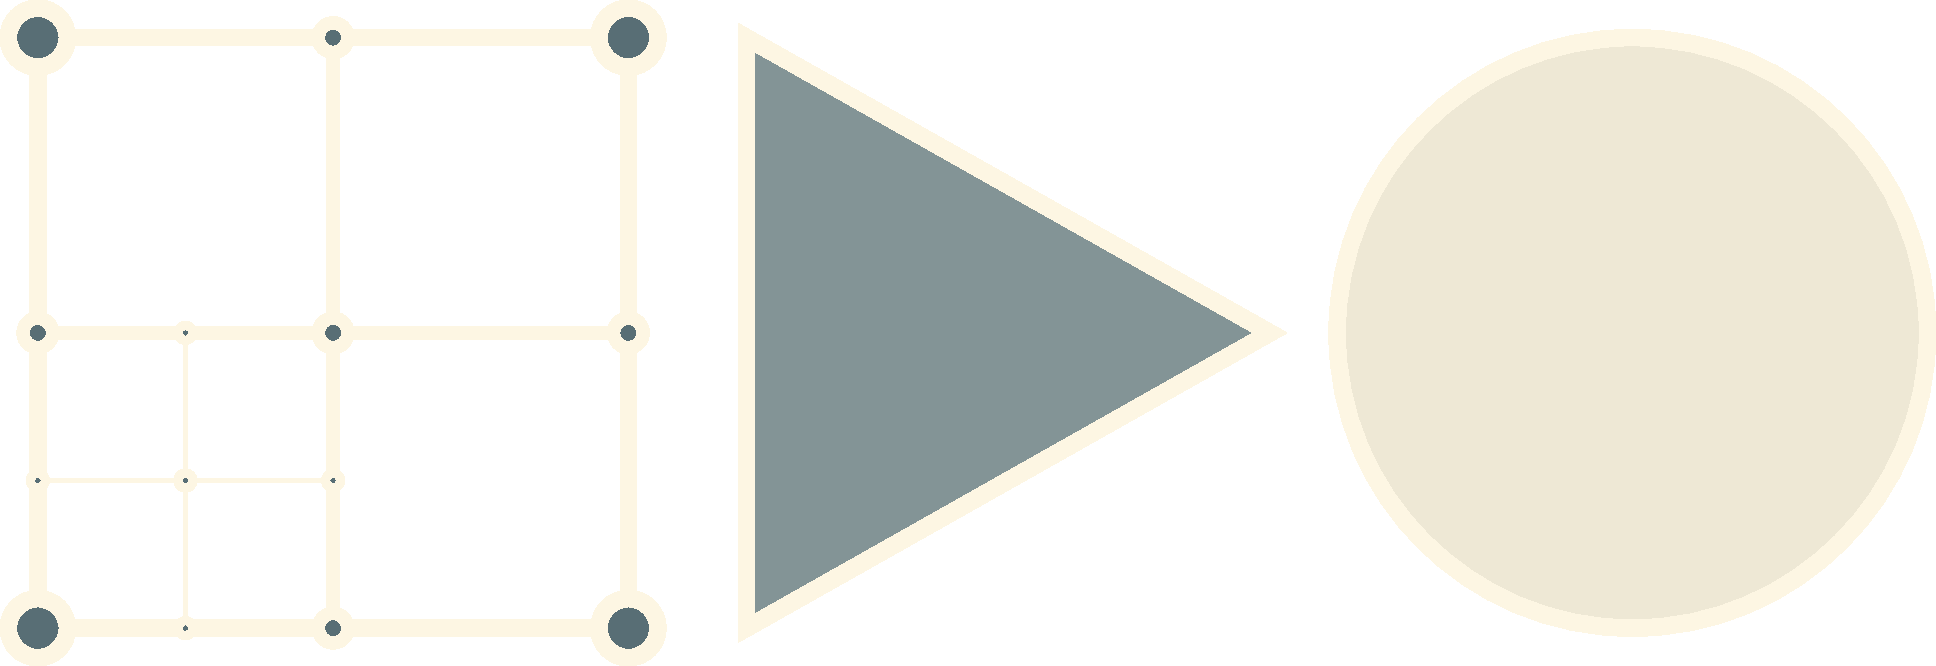
\includegraphics[width=42pt]{logo_slides}}}

%%%%%%%%%%%%%%%%%%%%%%%%%%%%%%%%%%%%%%%%%%%%%%%%%%%%%%%%%%%%%%%%%%%%%%%%%%%%%%%%

\newcommand{\PETSc}{\textsc{PETSc}}
\newcommand{\StagBL}{\textsc{StagBL}}
\newcommand{\StagYY}{StagYY}

%%%%%%%%%%%%%%%%%%%%%%%%%%%%%%%%%%%%%%%%%%%%%%%%%%%%%%%%%%%%%%%%%%%%%%%%%%%%%%%%

\author[Patrick Sanan]{Patrick Sanan}
\institute[]{ETH Zurich}

%%%%%%%%%%%%%%%%%%%%%%%%%%%%%%%%%%%%%%%%%%%%%%%%%%%%%%%%%%%%%%%%%%%%%%%%%%%%%%%%

\title{StagBL Tutorial}
\date[2020.03.04]{Staggered Grid Geodynamics Workshop, March 4-5, 2020}

%%%%%%%%%%%%%%%%%%%%%%%%%%%%%%%%%%%%%%%%%%%%%%%%%%%%%%%%%%%%%%%%%%%%%%%%%%%%%%%%

\begin{document}
\setbeamertemplate{section page}[customsection]
\setbeamertemplate{subsection page}[customsubsection]

%%%%%%%%%%%%%%%%%%%%%%%%%%%%%%%%%%%%%%%%%%%%%%%%%%%%%%%%%%%%%%%%%%%%%%%%%%%%%%%%
%%%%%%%%%%%%%%%%%%%%%%%%%%%%%%%%%%%%%%%%%%%%%%%%%%%%%%%%%%%%%%%%%%%%%%%%%%%%%%%%
\begin{frame}[fragile]
\titlepage
\begin{center}
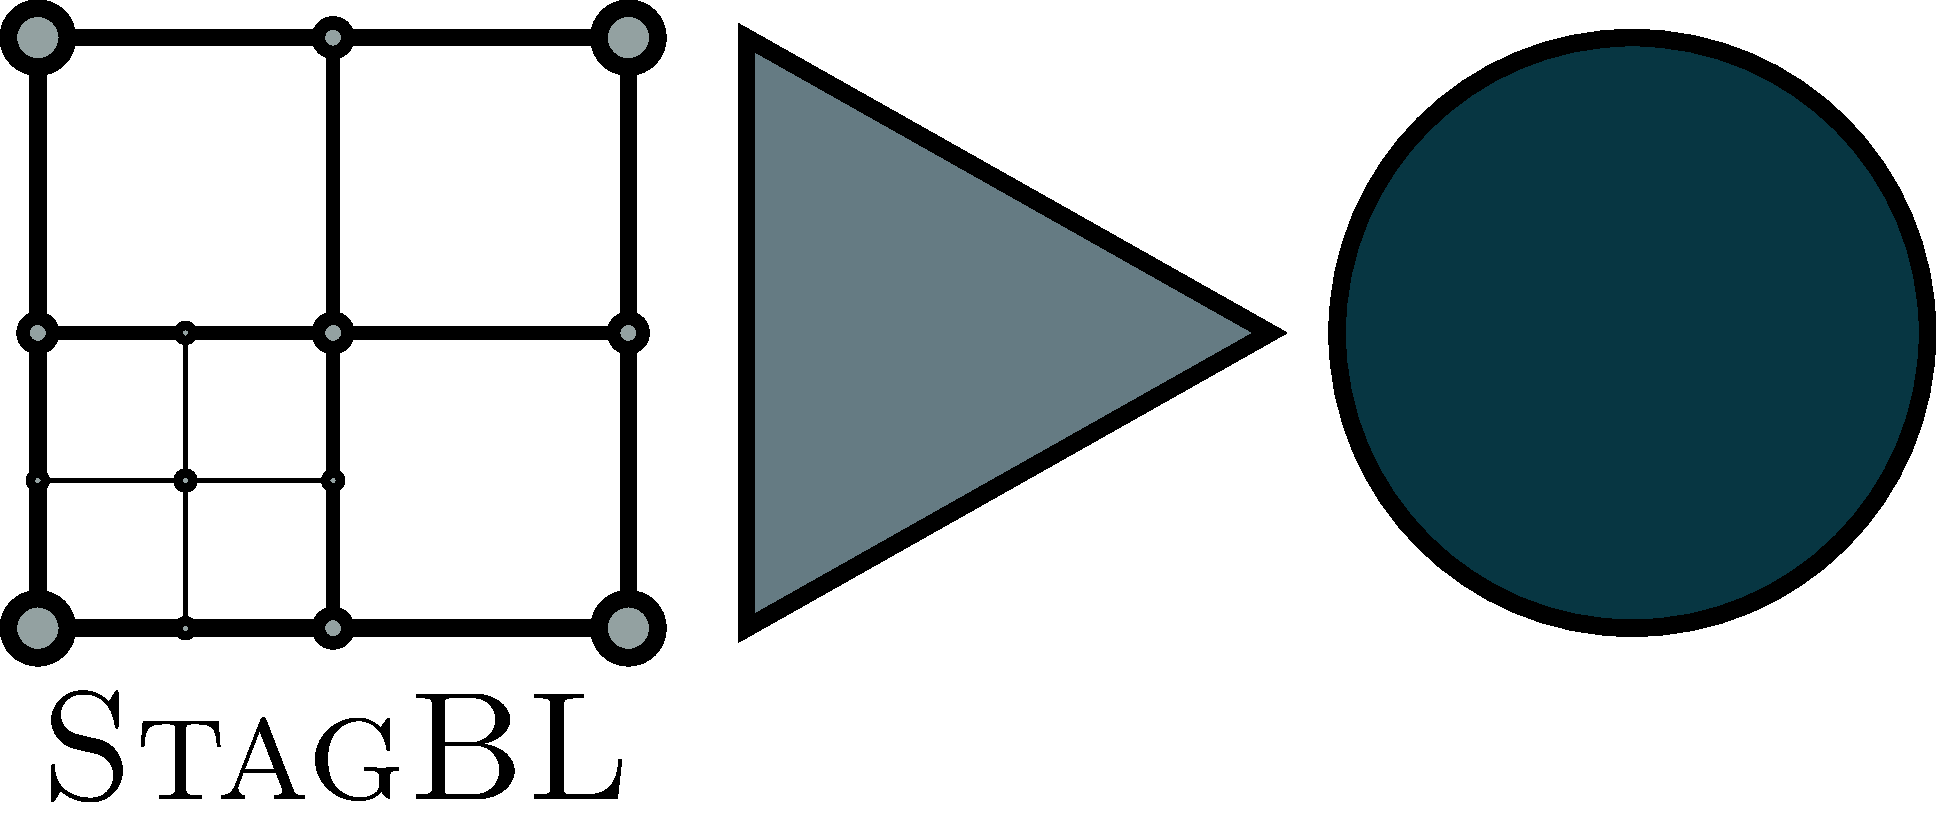
\includegraphics[height=0.125\textheight]{logo}
\end{center}
\begin{center}
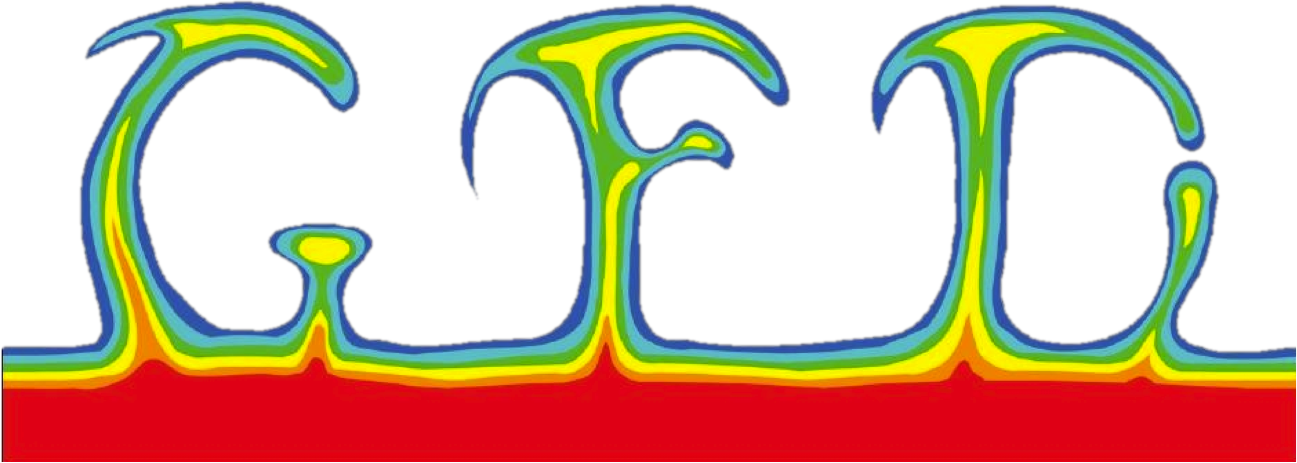
\includegraphics[height=1.6em]{GFD_t}
\hspace{2pt}
\raisebox{0.3em}{

\includegraphics[height=1em]{eth_logo_kurz_pos.pdf}}
\hspace{4pt}

\includegraphics[height=1.6em]{pasc_avec}
\hspace{2pt}

\includegraphics[height=1.6em]{CSCS_RGB}
\end{center}
\end{frame}

%%%%%%%%%%%%%%%%%%%%%%%%%%%%%%%%%%%%%%%%%%%%%%%%%%%%%%%%%%%%%%%%%%%%%%%%%%%%%%%%
%%%%%%%%%%%%%%%%%%%%%%%%%%%%%%%%%%%%%%%%%%%%%%%%%%%%%%%%%%%%%%%%%%%%%%%%%%%%%%%%
\begin{frame}[fragile]
\frametitlelogo{Outline}
\tableofcontents
\end{frame}

%%%%%%%%%%%%%%%%%%%%%%%%%%%%%%%%%%%%%%%%%%%%%%%%%%%%%%%%%%%%%%%%%%%%%%%%%%%%%%%%
%%%%%%%%%%%%%%%%%%%%%%%%%%%%%%%%%%%%%%%%%%%%%%%%%%%%%%%%%%%%%%%%%%%%%%%%%%%%%%%%
\section{\StagBL{}: Motivating Applications and Challenges}

%%%%%%%%%%%%%%%%%%%%%%%%%%%%%%%%%%%%%%%%%%%%%%%%%%%%%%%%%%%%%%%%%%%%%%%%%%%%%%%%
\begin{frame}[fragile]
\frametitle{Motivating Challenges from Mantle and Lithospheric Dynamics}
\begin{itemize}
\item Direct physical modelling of the viscous deformation of large parts of rocky planets, over the longest geological timescales (millions and billions of years)
\begin{itemize}
\item Mantle convection
\item Plate tectonics
\item Planetary formation
\end{itemize}
\item Multiple space/time scales, coupling to other systems, complex local physics/chemistry $\rightarrow$ large demand for computational resources
\end{itemize}
  \begin{center}

    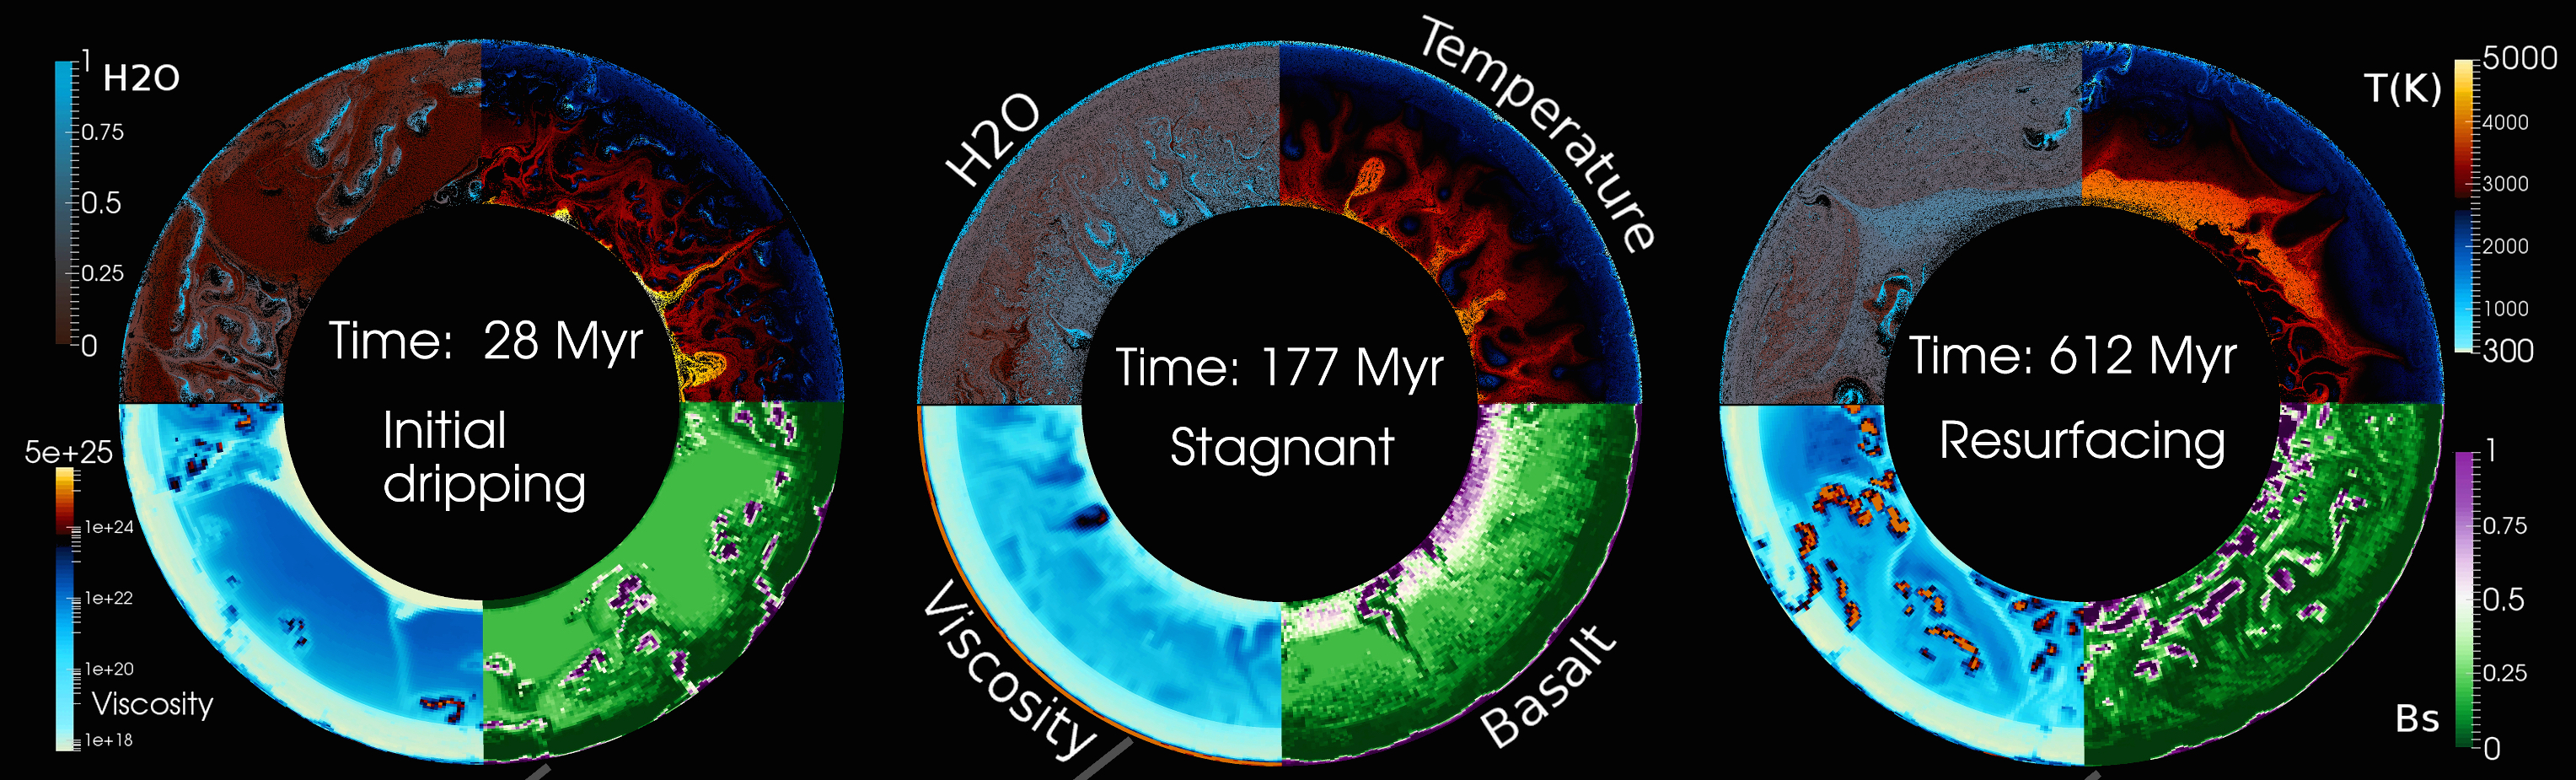
\includegraphics[width=0.5\textwidth]{images/rozel.jpg}\footfullcite{RozelEtAl2017}
    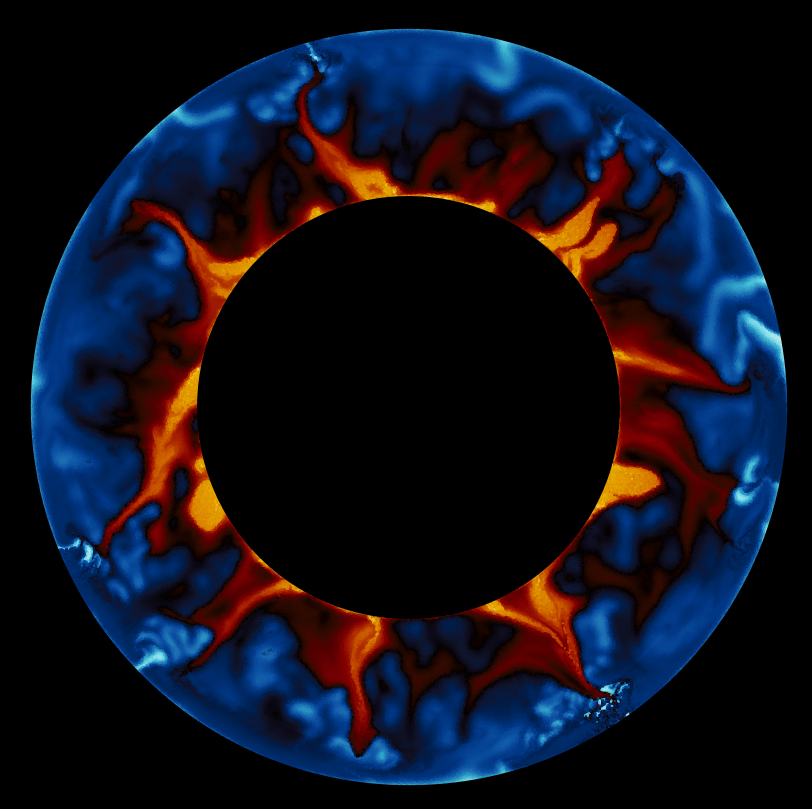
\includegraphics[width=0.12\textwidth]{images/frame_00030049_cut.png}
    %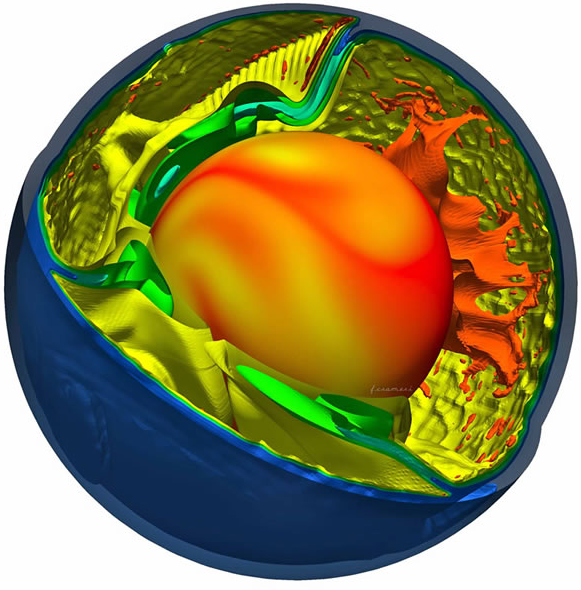
\includegraphics[width=0.14\textwidth]{images/crameri3.png}
    %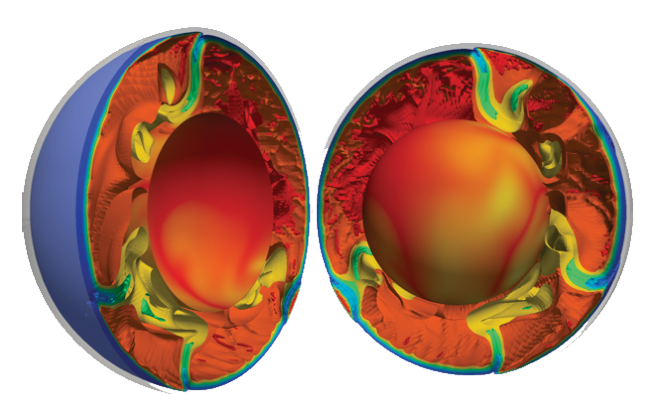
\includegraphics[width=0.25\textwidth]{images/Crameri2013.png}\footnote{Fabio Crameri}
    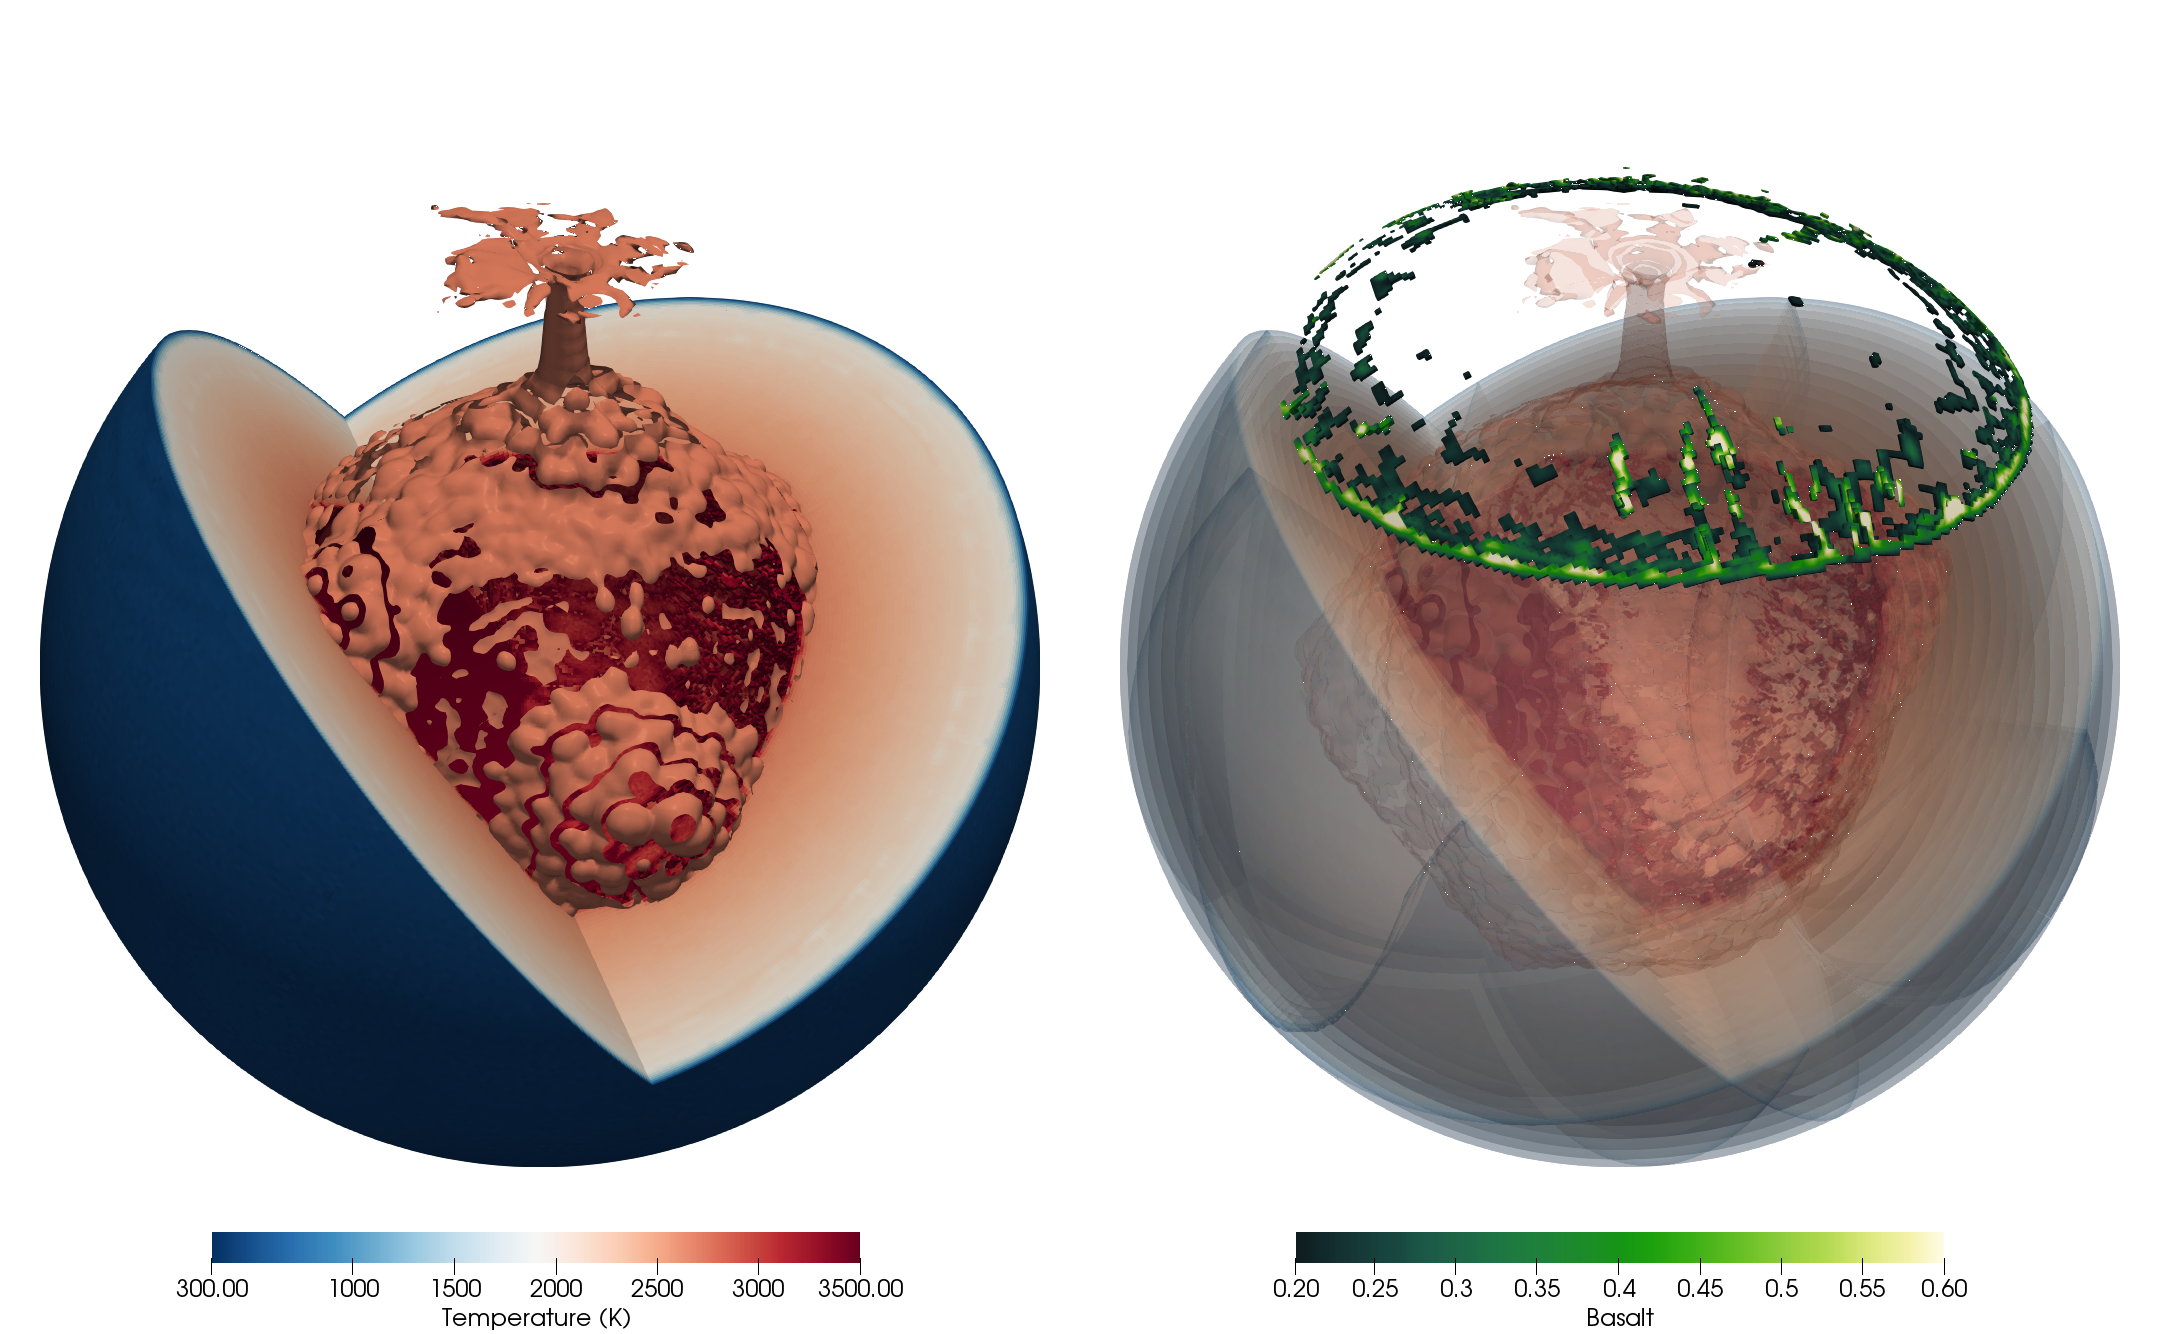
\includegraphics[width=0.25\textwidth]{images/YY-step60-BluRed_lowres.png}\footnote{Simulation by Charitra Jain (University of Durham)}
  \end{center}

\end{frame}

%%%%%%%%%%%%%%%%%%%%%%%%%%%%%%%%%%%%%%%%%%%%%%%%%%%%%%%%%%%%%%%%%%%%%%%%%%%%%%%%
\begin{frame}[fragile]
\frametitlelogo{Motivating Physics and Discretization}
\small
\begin{itemize}
\item Conservation of mass and momentum
$$
\nabla \cdot (\rho v) = 0, \quad \quad
\nabla \cdot \sigma - \nabla p = \frac{\text{Ra} \hat r \rho}{\Delta \rho_{\text{thermal}}}
$$
  \item Conservation of Energy
$$
\rho C_p \frac{DT}{Dt} = -\text{Di}_s\alpha \rho T v_r + \nabla \cdot (k \nabla T) + \rho H + \frac{\text{Di}_s}{\text{Ra}} \sigma : \dot \epsilon
$$
\item Advection of arbitrary Lagrangian quantities
$$
\frac{DC}{Dt} = 0
$$
\item Constitutive Relationship
$$
    \dot \epsilon \doteq \frac{1}{2}\left(\nabla u + (\nabla u)^T \right), \quad \sigma = \eta \dot \epsilon
$$
\end{itemize}
\end{frame}

%%%%%%%%%%%%%%%%%%%%%%%%%%%%%%%%%%%%%%%%%%%%%%%%%%%%%%%%%%%%%%%%%%%%%%%%%%%%%%%%
\begin{frame}[fragile]
\frametitlelogo{Motivating Physics and Discretization}
\small
\begin{itemize}
\item Staggered grid finite difference / finite volume methods:
Eulerian grid and
low order, narrow stencil\\
\begin{center}
  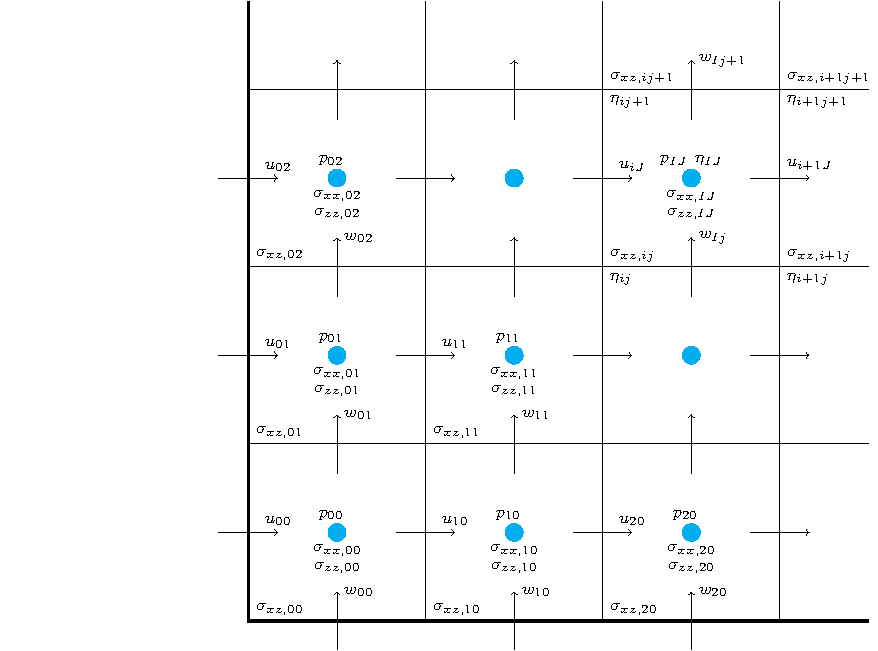
\includegraphics[width=0.2\textwidth]{images/StagGrid.pdf} \hspace{10pt}
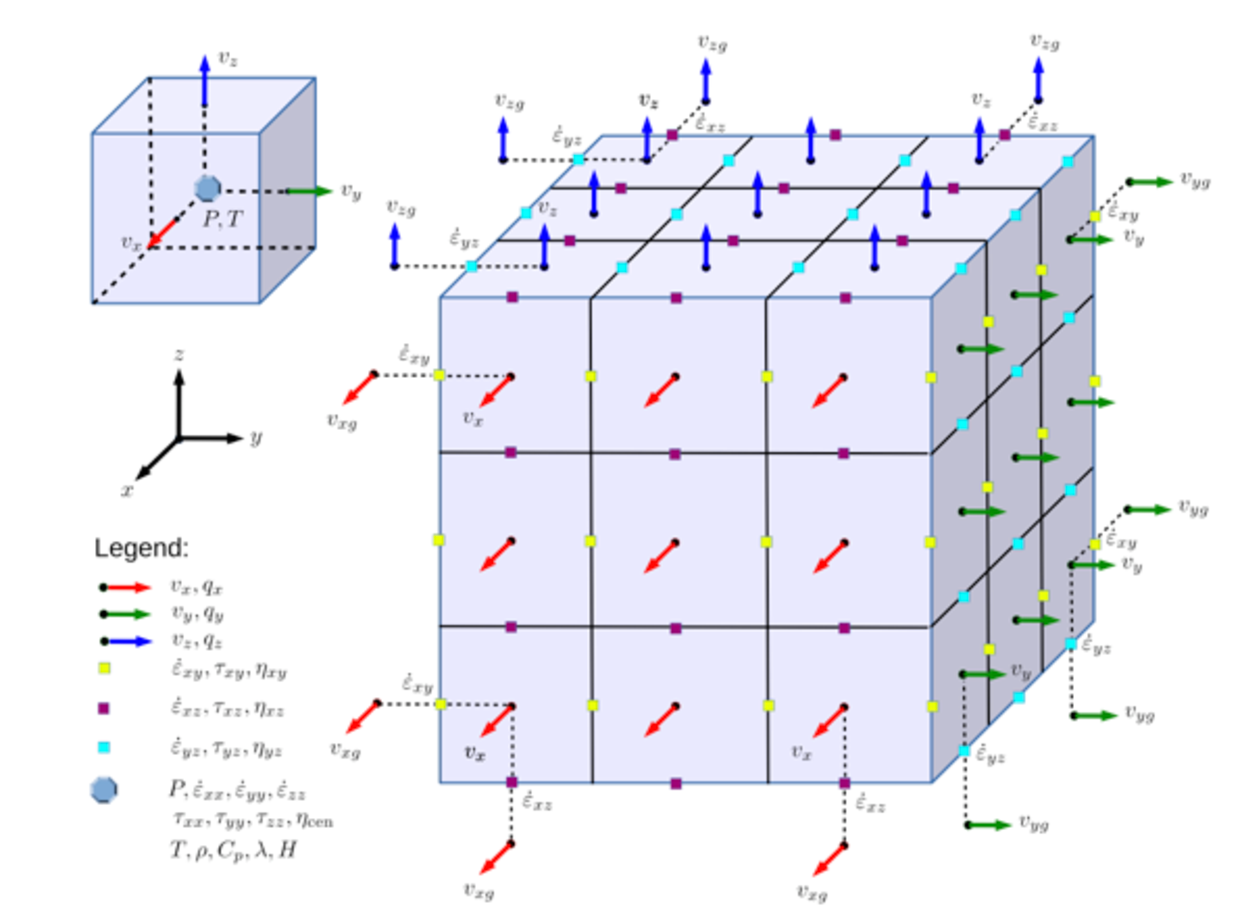
\includegraphics[width=0.3\textwidth]{images/KausEquations.pdf}\footfullcite{KausEtAl2016}
\end{center}
\item Particle-in-cell/MAC methods\footfullcite{HarlowWelch1965}
 ($\rightarrow$ arbitrary discontinuous viscosity field)
\item Critical computational step is solving saddle point Stokes linear systems
$$
\begin{bmatrix}
A 	&  G \\
D 	&
\end{bmatrix}
\begin{bmatrix}
u \\
p
\end{bmatrix}
=
\begin{bmatrix}
f \\
0
\end{bmatrix},
\quad \text{or } \mathcal{A} v = {\mathcal F}
$$
\end{itemize}
\end{frame}

%%%%%%%%%%%%%%%%%%%%%%%%%%%%%%%%%%%%%%%%%%%%%%%%%%%%%%%%%%%%%%%%%%%%%%%%%%%%%%%%
\section{The \StagBL{} Project}

%%%%%%%%%%%%%%%%%%%%%%%%%%%%%%%%%%%%%%%%%%%%%%%%%%%%%%%%%%%%%%%%%%%%%%%%%%%%%%%%
\begin{frame}[fragile]
\frametitlelogo{Mantle and Lithospheric Dynamics Codes}
\begin{minipage}{0.49\textwidth}
\StagYY{} \\
  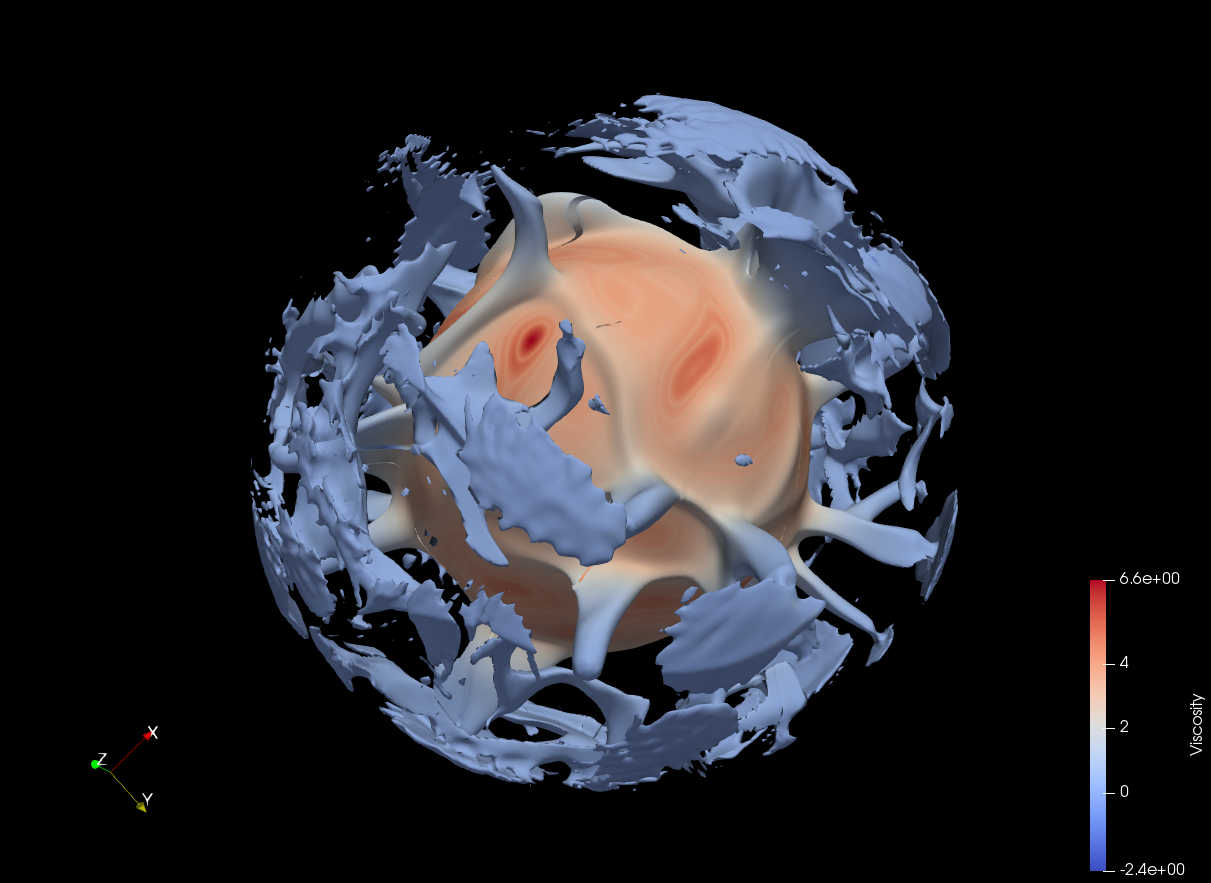
\includegraphics[width=0.7\textwidth]{images/martina_1_placeholder.png}
\textsc{LaMEM}\footnotemark\\
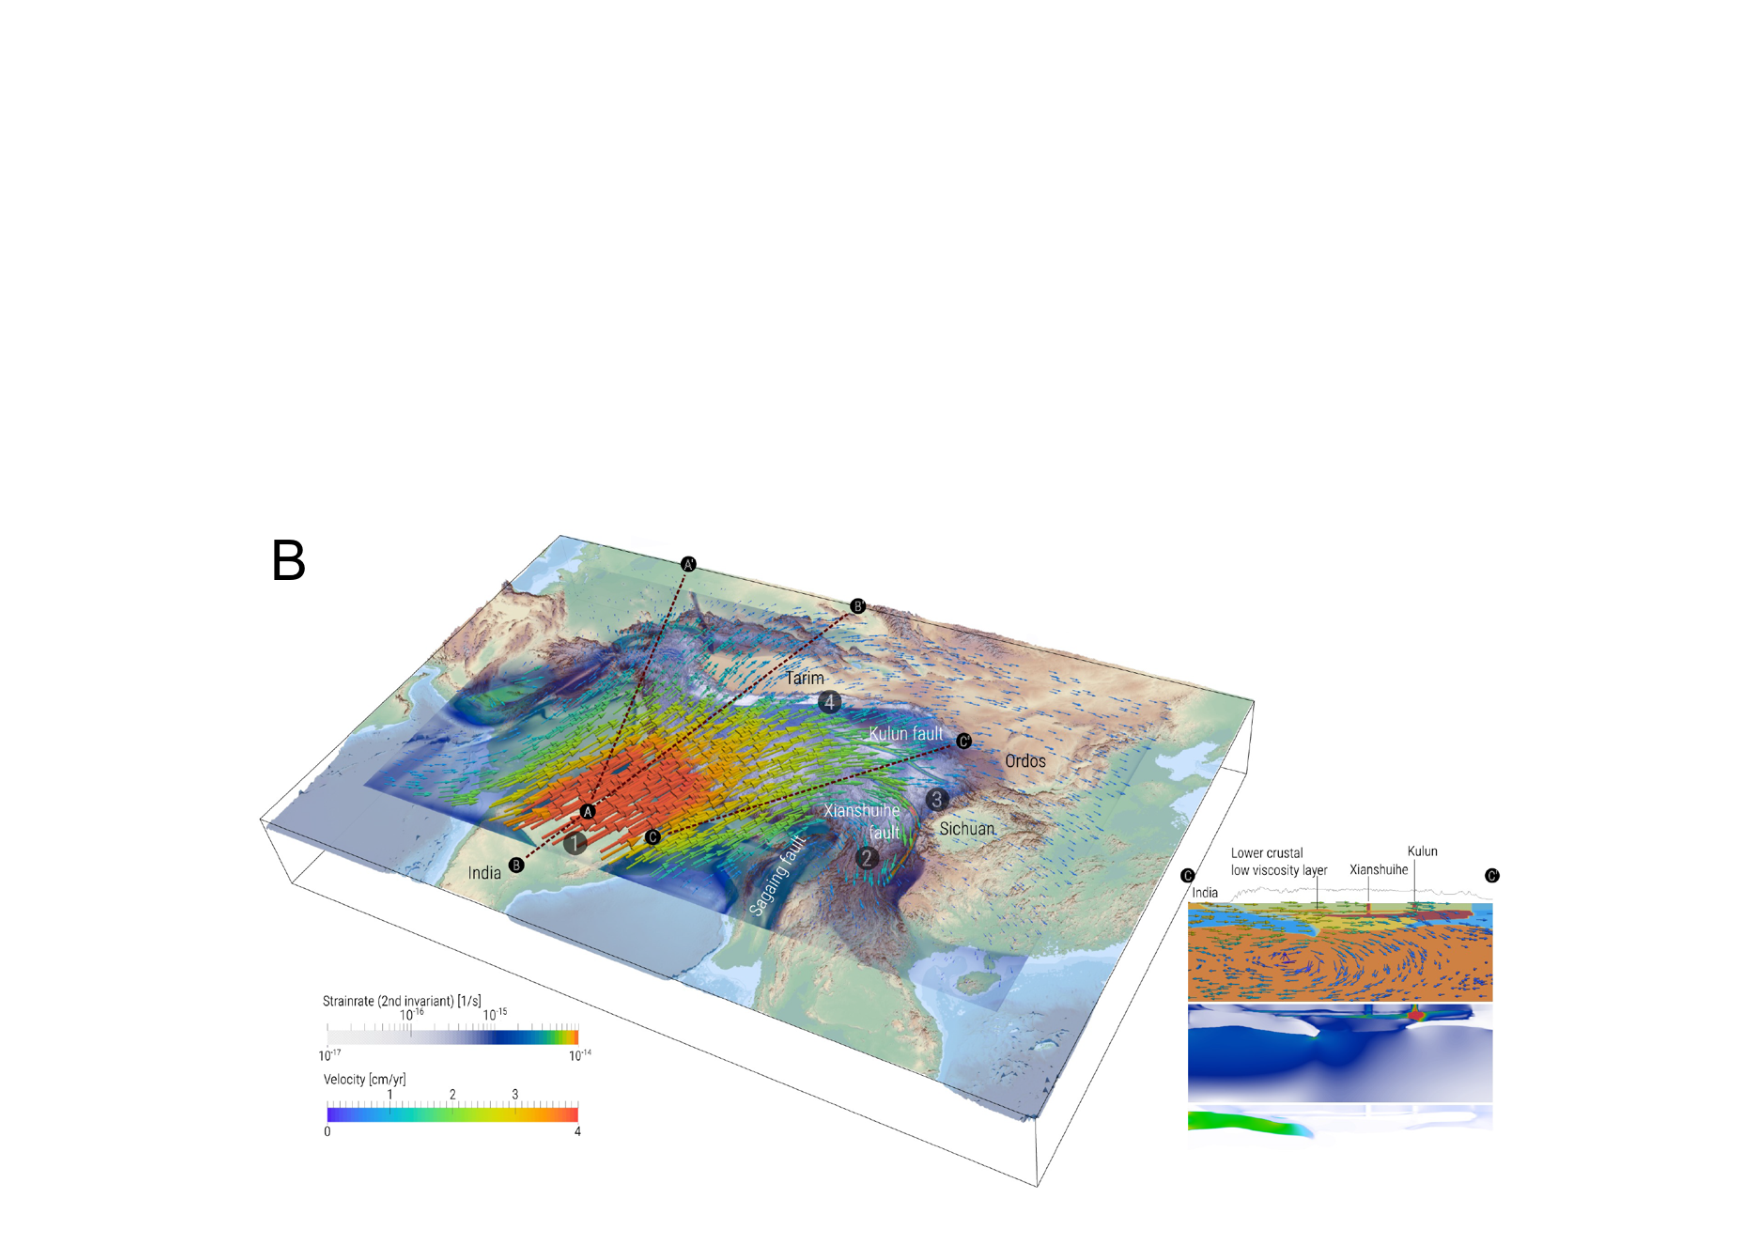
\includegraphics[width=0.7\textwidth]{images/kausB.pdf}
\end{minipage}
\begin{minipage}{0.49\textwidth}
\textsc{I3ELVIS}\footnotemark\\
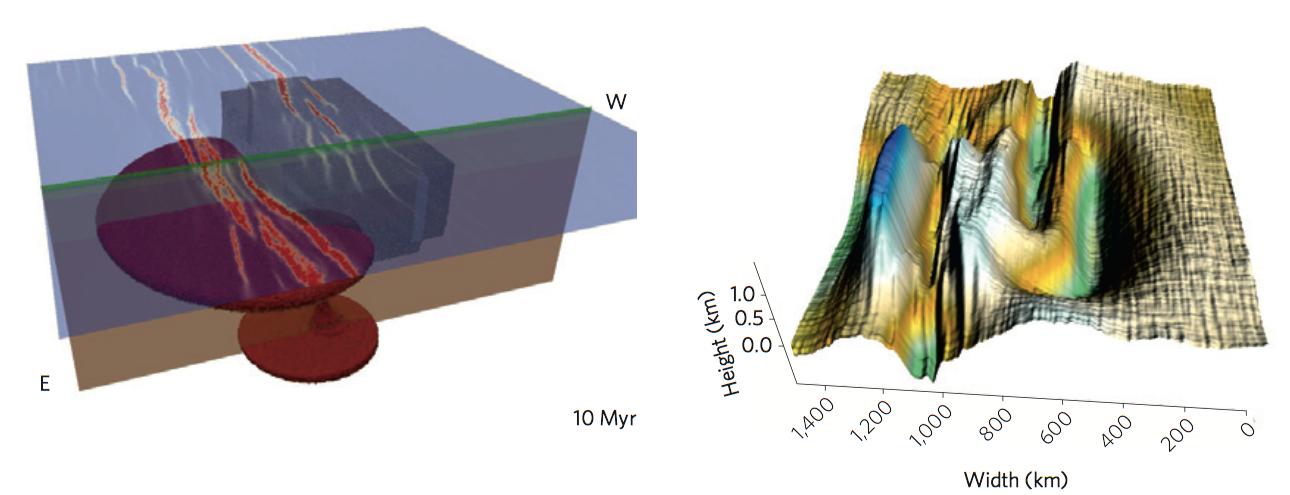
\includegraphics[width=0.7\textwidth]{images/ngeo.png}
\textsc{I3ELVIS\_planet} \footnotemark\\
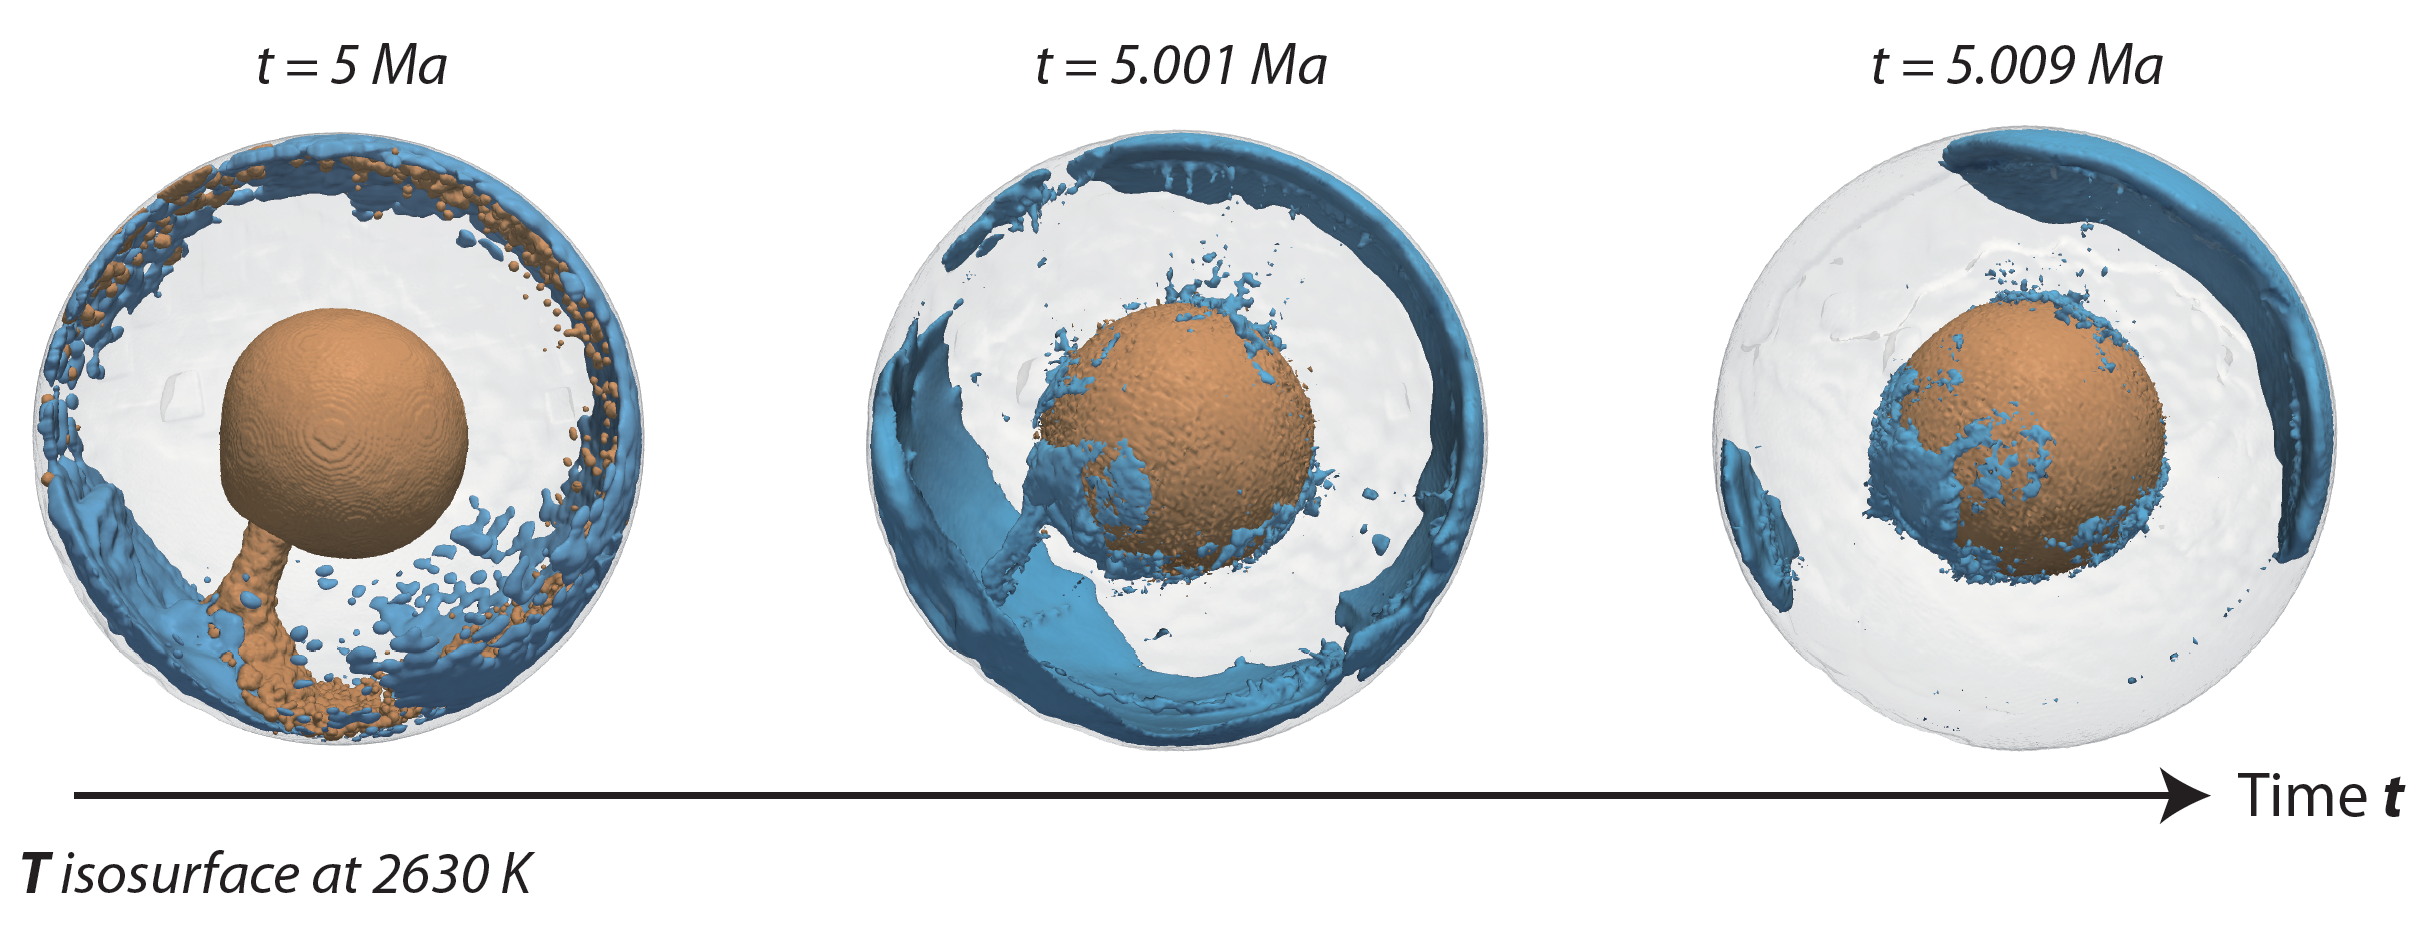
\includegraphics[width=0.7\textwidth]{images/gregor.png}\\
Plus, many others in geodynamics and far beyond.
%Many other application areas in computational science use data on regular square/hex cell complexes (athmospheric, magnetotellurics, CFD, MHD, etc.
\end{minipage}
\footnotetext{\url{https://bitbucket.org/bkaus/lamem}, \fullcite{PusokKaus2015}}
\footnotetext{\fullcite{GeryaYuen2007}}
\footnotetext{\fullcite{GolabekEtAl2009}}
\end{frame}

%%%%%%%%%%%%%%%%%%%%%%%%%%%%%%%%%%%%%%%%%%%%%%%%%%%%%%%%%%%%%%%%%%%%%%%%%%%%%%%%
\begin{frame}[fragile]
\frametitlelogo{Bottlenecks}
\begin{itemize}
\item non-uniform performance
\item not all codes can be arbitrarily parallelized
\item not all codes can leverage composable solvers
\item codes can't share optimized operations
\end{itemize}
\end{frame}

%%%%%%%%%%%%%%%%%%%%%%%%%%%%%%%%%%%%%%%%%%%%%%%%%%%%%%%%%%%%%%%%%%%%%%%%%%%%%%%%
\begin{frame}[fragile]
  \frametitlelogo{\StagBL{} PASC Project}
\begin{itemize}
\item Staggered-grid FD plus particle advection is a useful, efficient, and widely-used tool, worthy of a more robust library implementation.
\item Low-hanging fruit in accelerating the work of users of 3 application codes as they push the boundaries of their research topics.
\item People want solver options, hence need a uniform interface to them
\item Address the bottleneck between geodynamics researchers and supercomputers: ``Path to performance''from the textbook
  \begin{center}
  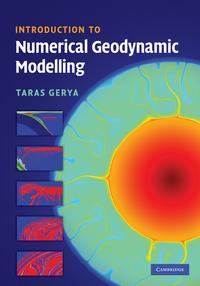
\includegraphics[height=20px]{geryabook} \begin{minipage}{20px}\scalebox{1}{$\rightarrow$}\vspace{10px}\end{minipage}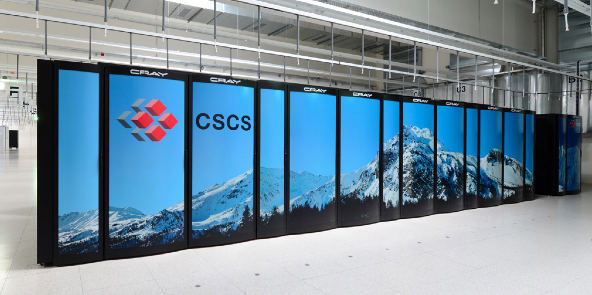
\includegraphics[height=20px]{daint}
  \end{center}
\item Better analysis tools for multigrid (non-)convergence are needed in the broader community.
\item AMR has many potential applications, but needs focused attention to develop and implement for FD grids.
\item Inverse modeling: many forward runs incentivize optimization of kernels.
\end{itemize}
\end{frame}

%%%%%%%%%%%%%%%%%%%%%%%%%%%%%%%%%%%%%%%%%%%%%%%%%%%%%%%%%%%%%%%%%%%%%%%%%%%%%%%%
\begin{frame}[fragile]
  \frametitlelogo{\StagBL{} Design}
  \begin{itemize}
  \item Central driver: simplicity
  \item Written in C, with simple object-oriented design
  \item Focus on components required for efficient, flexible Stokes solvers used by MAC-style geodynamics applications
  \item Use external libraries whenever possible
  \item Four core classes
  \item Modern software engineering practices (version control, portable build, tests)
  \item Configure/build: simple GNUMake-based approach, inspired by HPGMG\footnote{\url{https://hpgmg.org}}
  \item Testing: simple, custom test harness\footnote{With Dave May, \url{https://bitbucket.org/dmay/pythontestharness} (big update underway)}, designed for ease of testing MPI-based scientific codes on local machines and clusters with batch systems
  \item Document by example, using included demo mini-apps
  \end{itemize}
\end{frame}

%%%%%%%%%%%%%%%%%%%%%%%%%%%%%%%%%%%%%%%%%%%%%%%%%%%%%%%%%%%%%%%%%%%%%%%%%%%%%%%%
\begin{frame}[fragile]
\frametitlelogo{\StagBL{} Project: Components}
\begin{center}
  \includegraphics[width=0.9\textwidth]{images/components.pdf}
\end{center}
\end{frame}

%%%%%%%%%%%%%%%%%%%%%%%%%%%%%%%%%%%%%%%%%%%%%%%%%%%%%%%%%%%%%%%%%%%%%%%%%%%%%%%%
\begin{frame}[fragile]
\frametitlelogo{\StagBL{} Website}
\begin{center}
  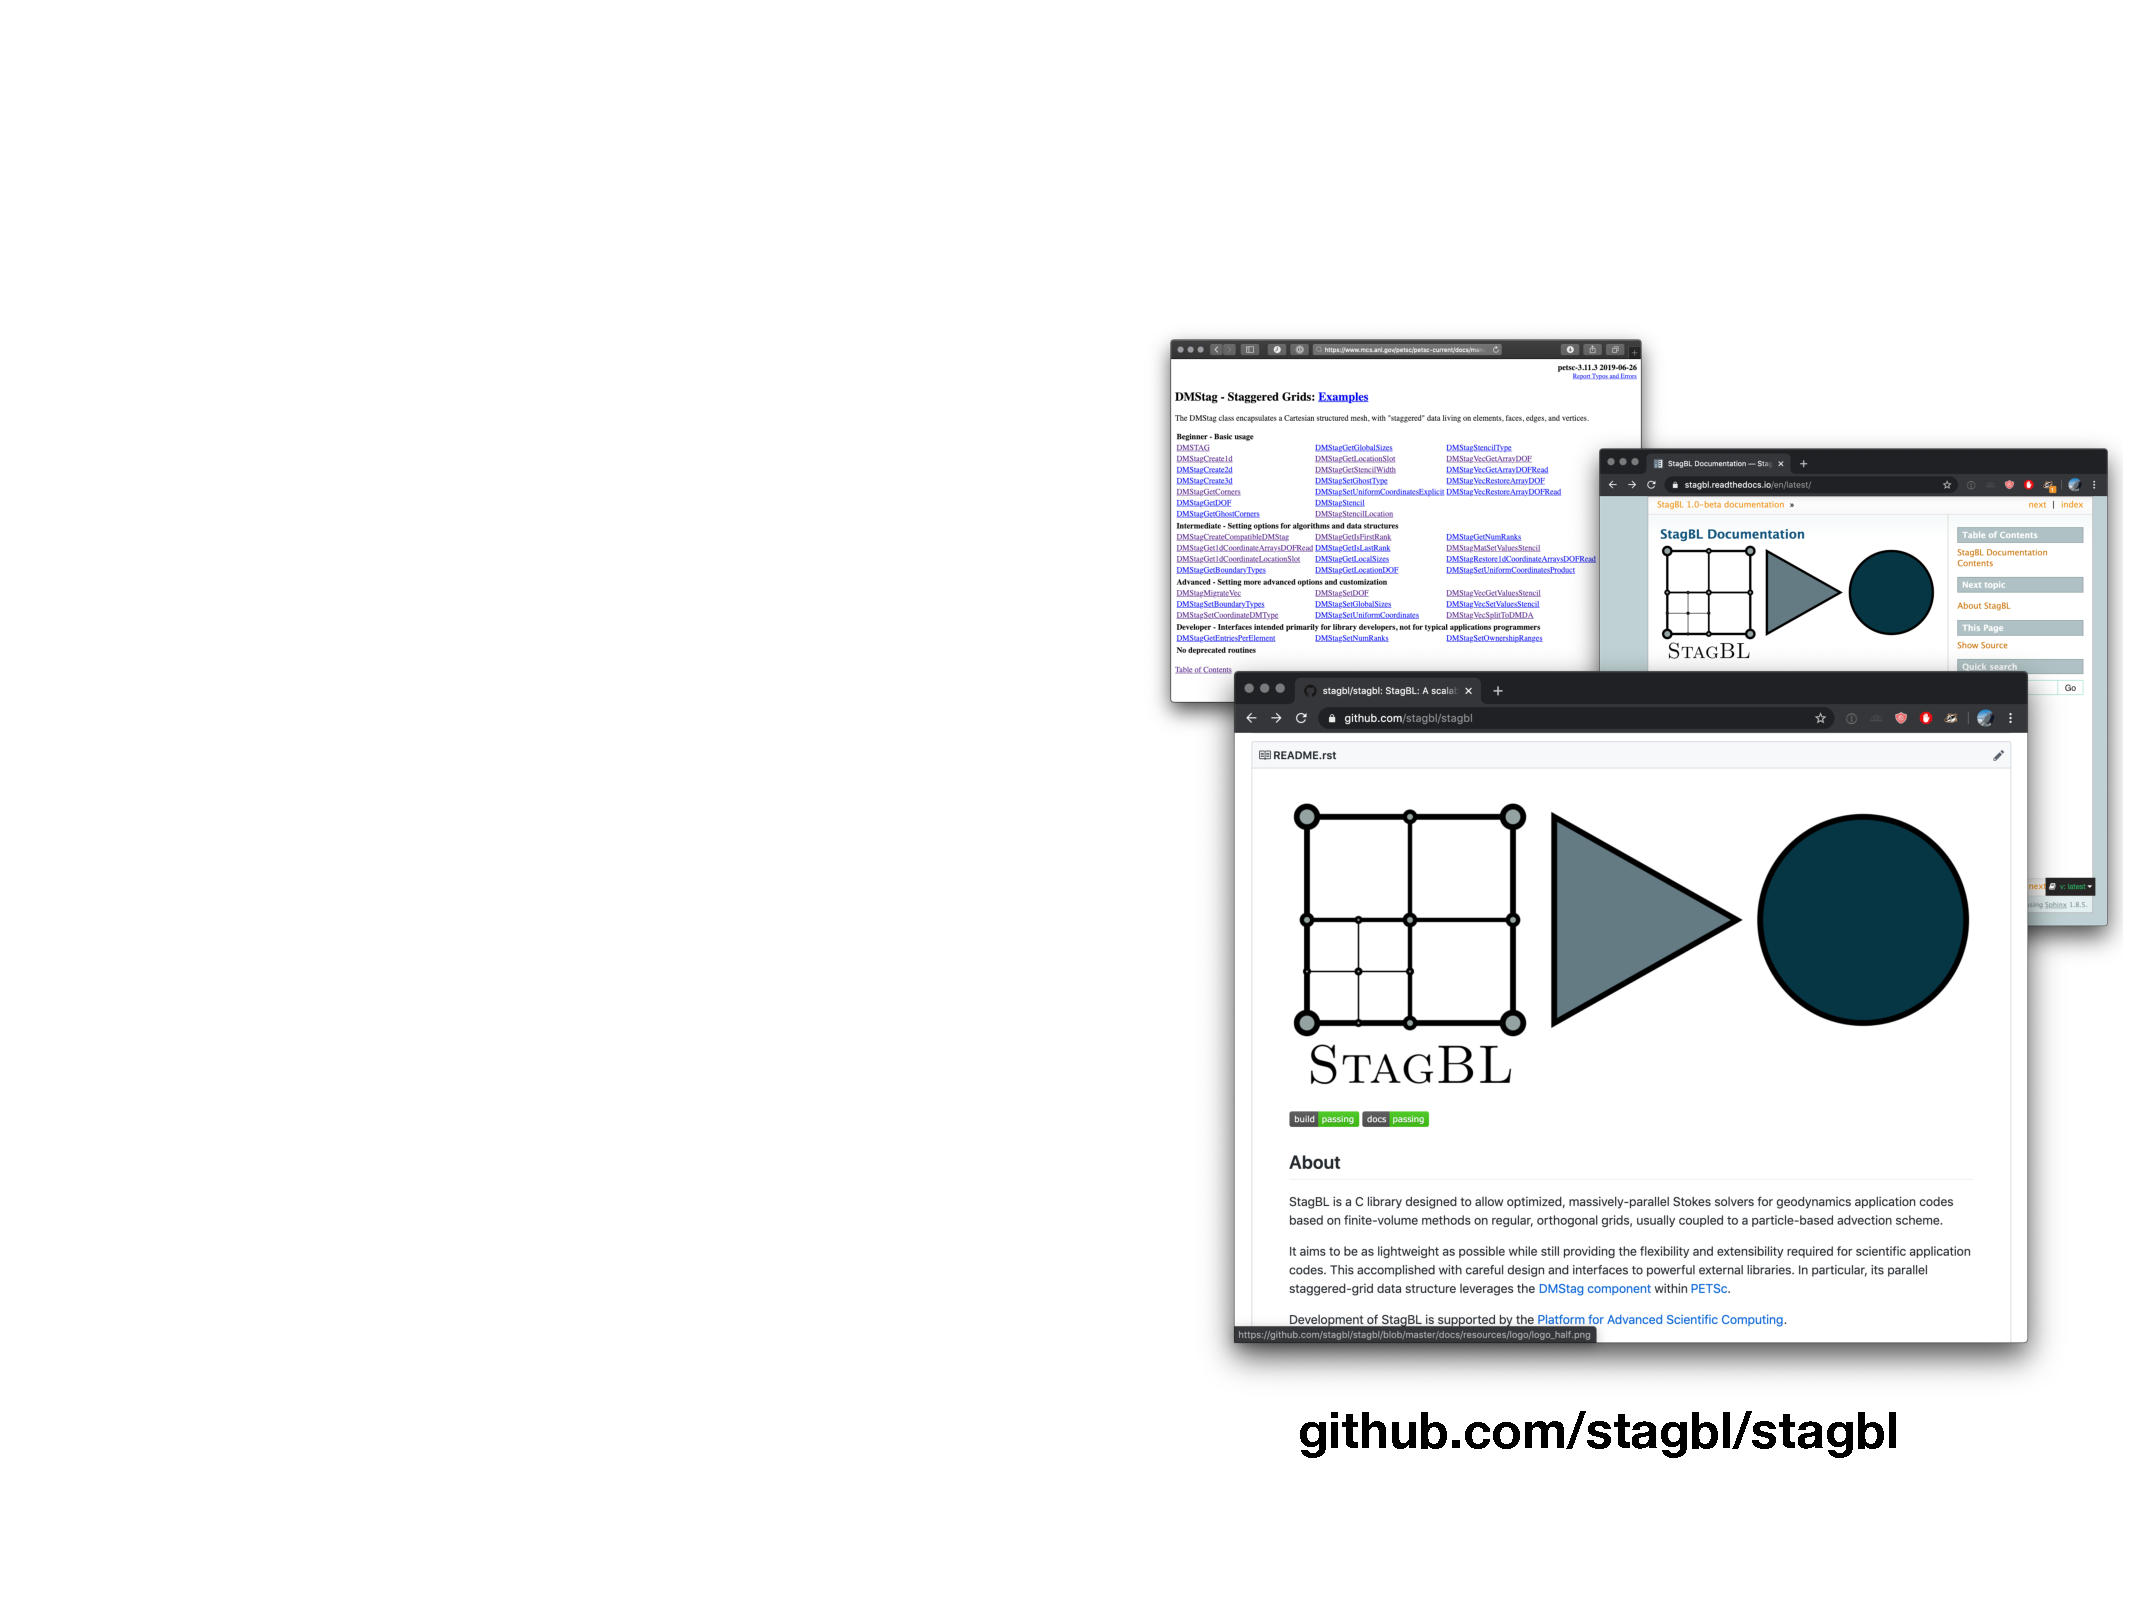
\includegraphics[height=0.8\textheight]{images/websites.pdf}
\end{center}
\end{frame}

%%%%%%%%%%%%%%%%%%%%%%%%%%%%%%%%%%%%%%%%%%%%%%%%%%%%%%%%%%%%%%%%%%%%%%%%%%%%%%%%
\section{\texttt{DMStag}}

%%%%%%%%%%%%%%%%%%%%%%%%%%%%%%%%%%%%%%%%%%%%%%%%%%%%%%%%%%%%%%%%%%%%%%%%%%%%%%%%
\begin{frame}[fragile]
\frametitlelogo{DMStag and \PETSc{} Integration}
\begin{itemize}
\item  \StagBL{} heavily leverages capabilities from the \PETSc{} library
\item The central object is \lstinline{DMStag}, a new \lstinline{DM} implementation
\item Available in PETSc 3.11\footnote{See \url{https://www.mcs.anl.gov/petsc/petsc-current/docs/manualpages/DMSTAG/index.html}} and under active development \footnote{contact \texttt{patrick.sanan@erdw.ethz.ch} with feature requests, etc.}.
\item We make heavy use of the notion of ``compatibility''to quantify the concept of two objects objects representing ``different data on the same domain''.
\end{itemize}
\end{frame}

%%%%%%%%%%%%%%%%%%%%%%%%%%%%%%%%%%%%%%%%%%%%%%%%%%%%%%%%%%%%%%%%%%%%%%%%%%%%%%%%
\begin{frame}[fragile]
\frametitlelogo{\PETSc{}}
\begin{center}
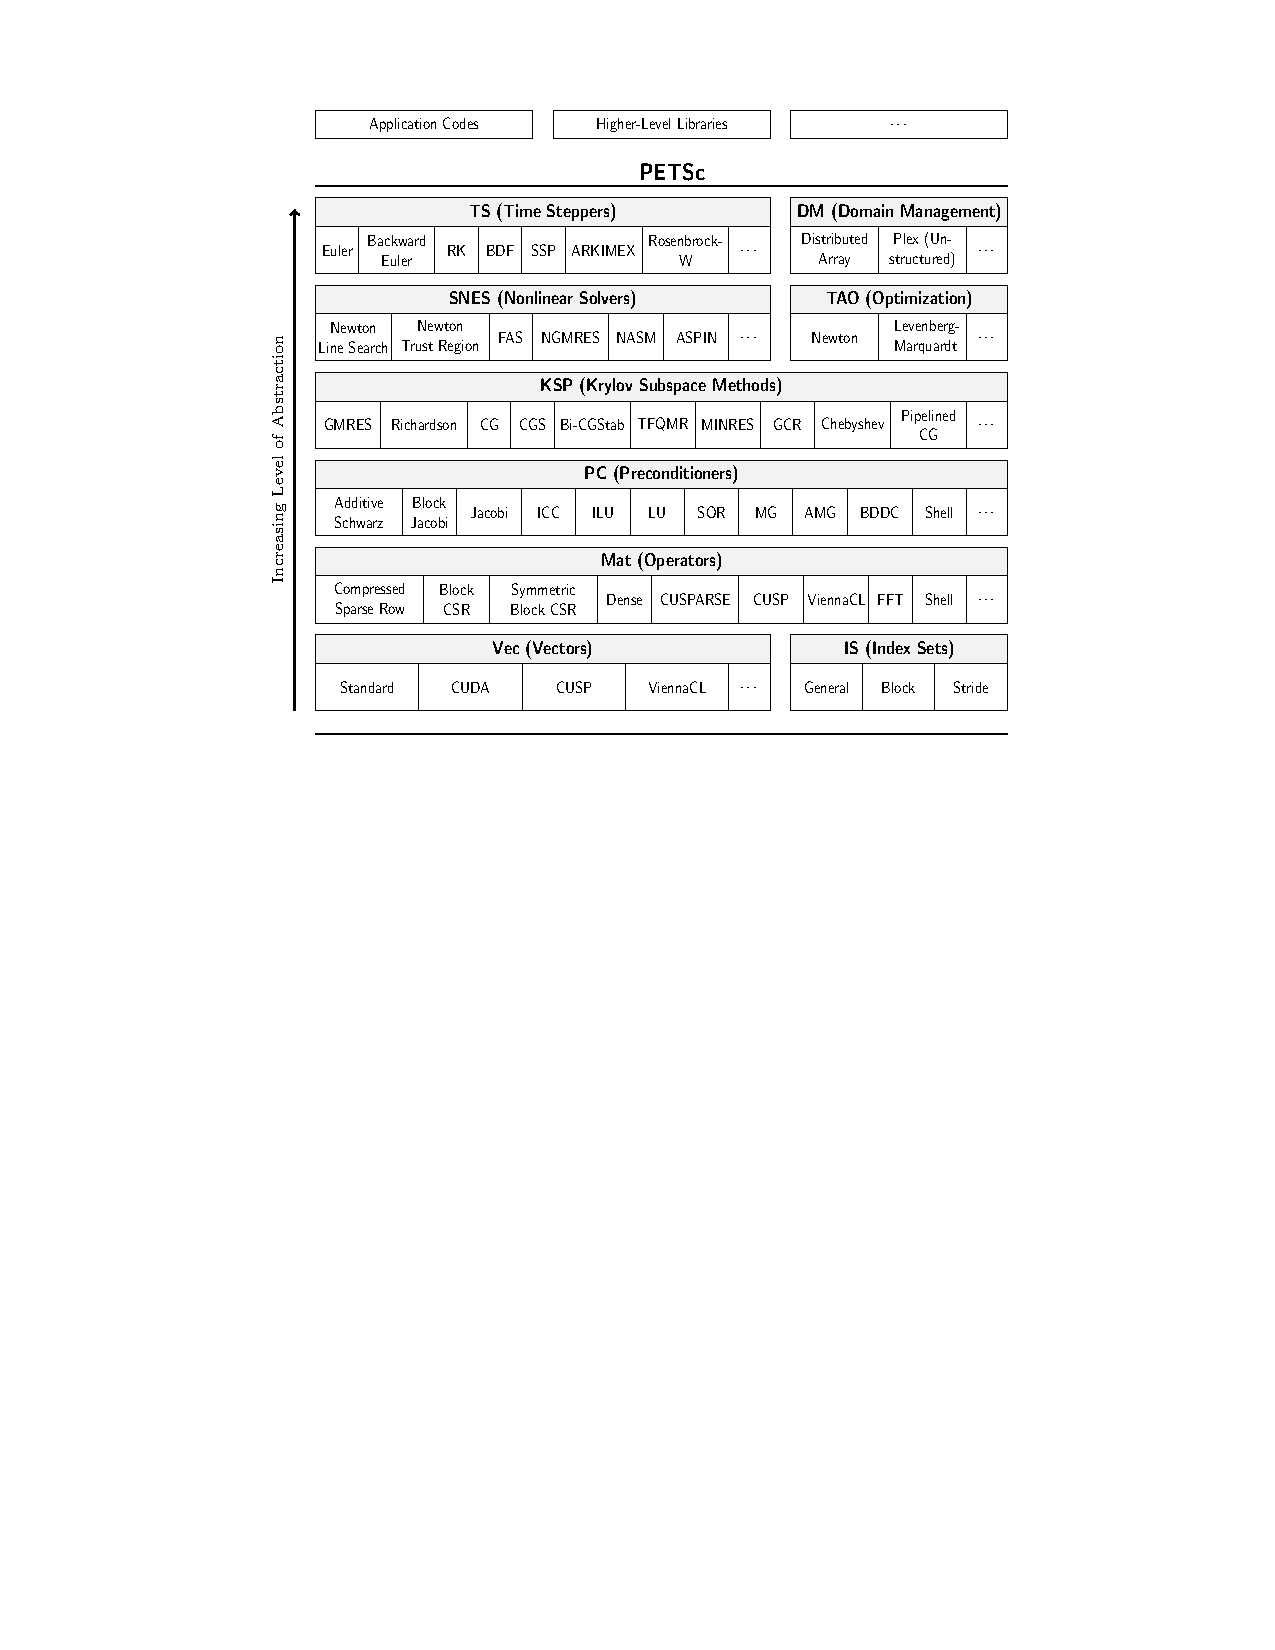
\includegraphics[height=0.4\textheight]{petsclibs}
\hspace{10pt}
\only<1>{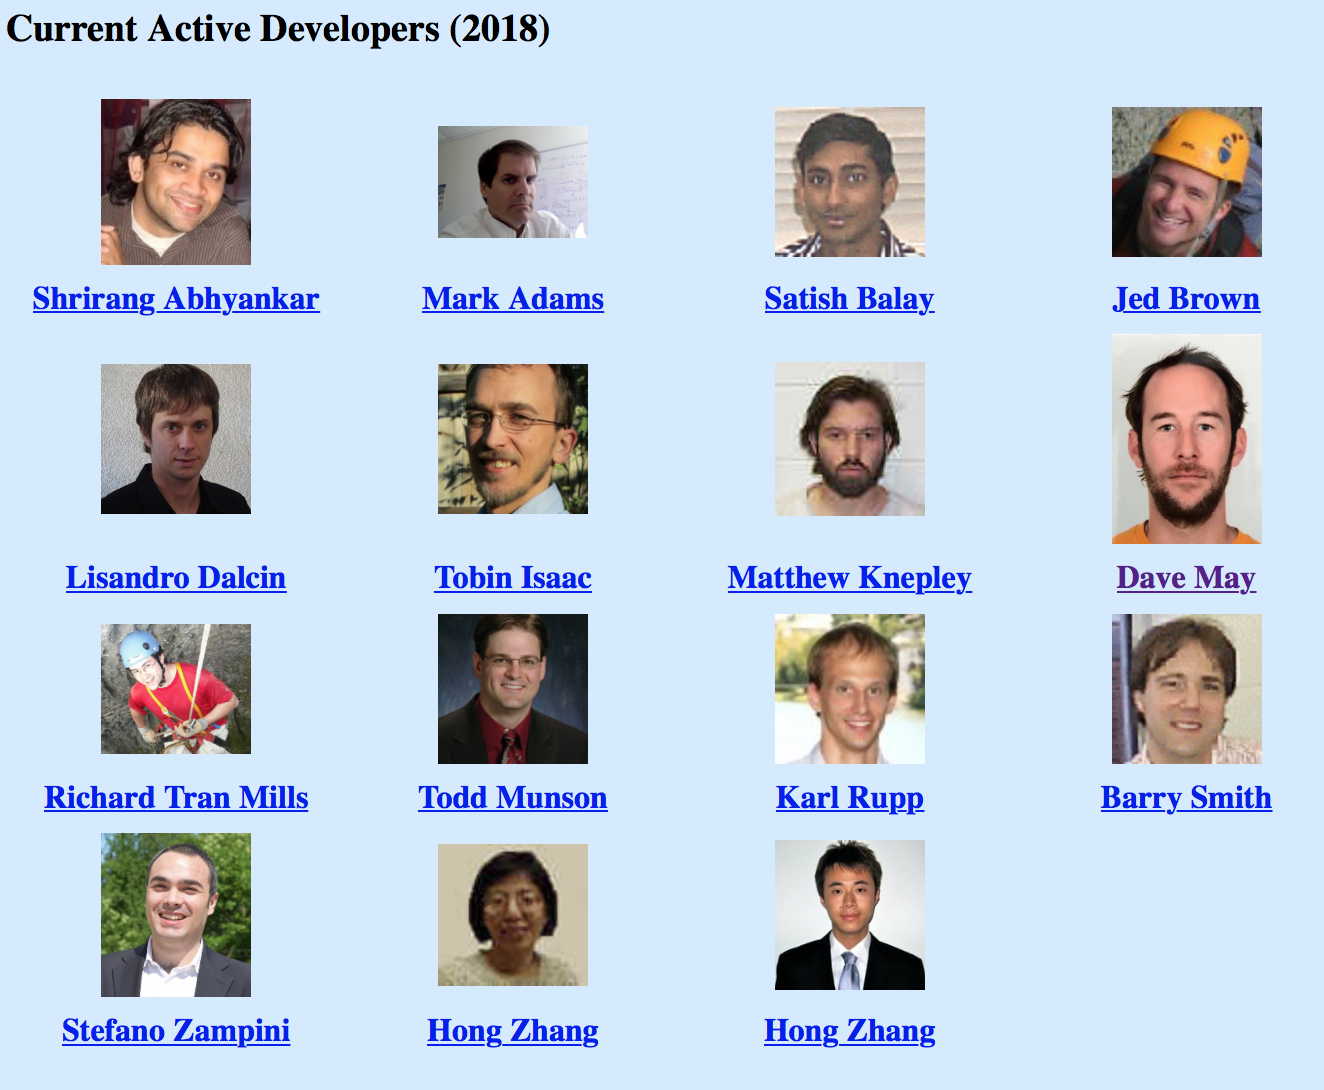
\includegraphics[height=0.4\textheight]{petscdevs}}
\only<2>{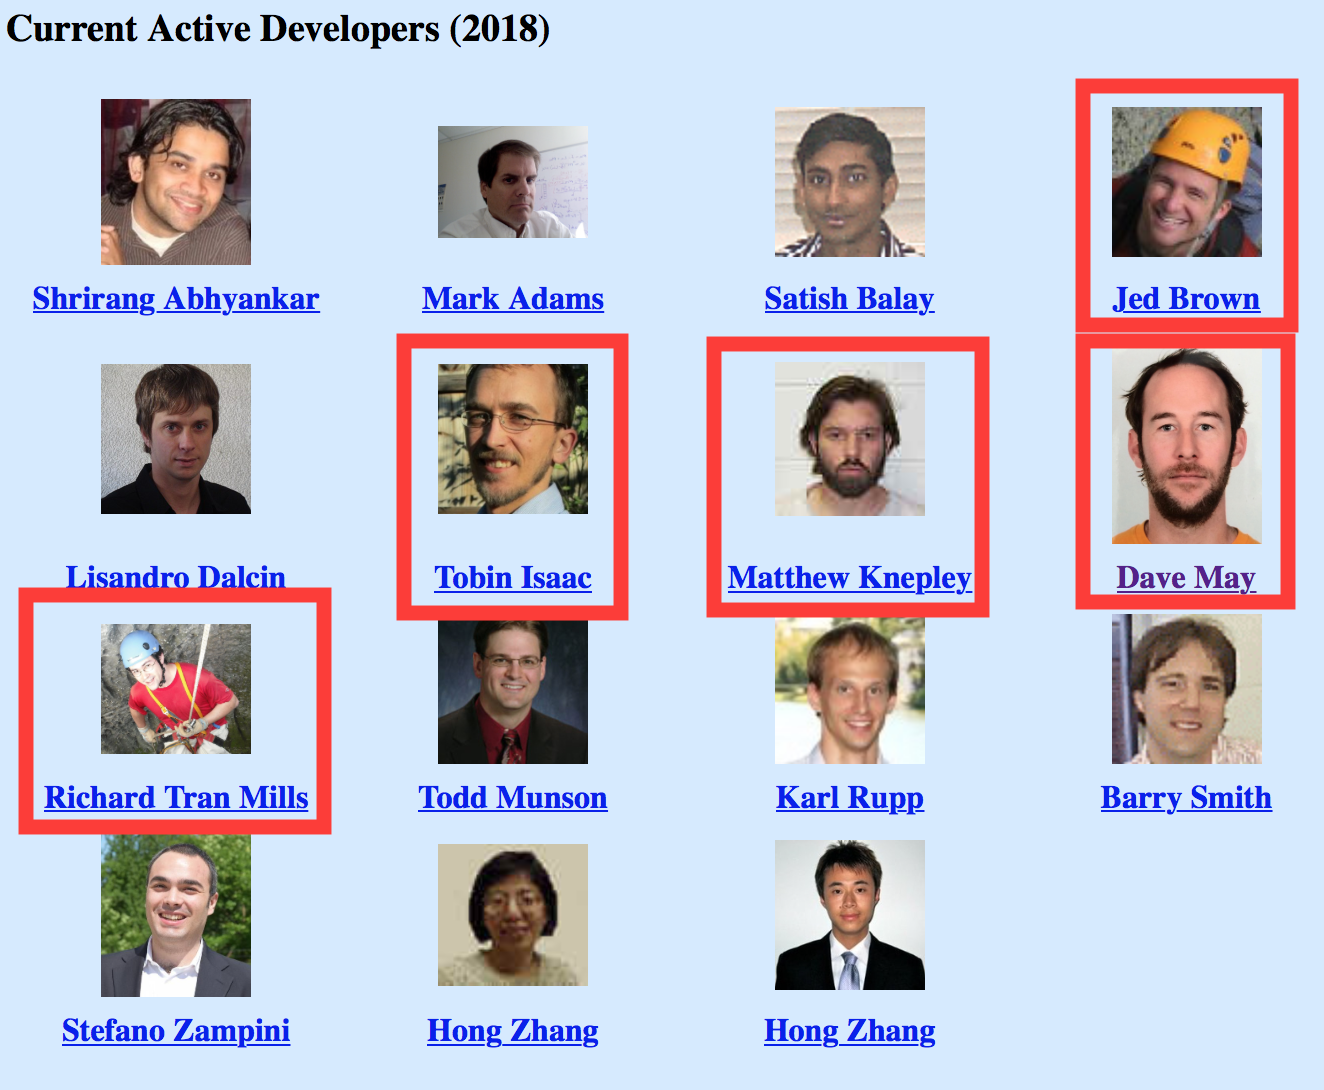
\includegraphics[height=0.4\textheight]{petscdevs_earth}}
\end{center}
\begin{itemize}
  \item ``\textbf{P}ortable, \textbf{E}xtensible \textbf{T}oolkit for \textbf{S}cientific \textbf{c}omputation (\textbf{P}ortable, \textbf{E}xtensible \textbf{T}oolkit for \textbf{S}olver \textbf{c}omposition?)
\item Efficient, scalable, parallel linear linear algebra and solvers
\item Open-source (2-clause BSD) C library (+ Fortran/Python bindings), built on \textsc{MPI}
\item Developed and (well-)supported for over 20 years at ANL, with an active community
\item Large, highly configurable, can download and install dependencies
%\item \textbf{Coming Soon} PETSc introductory tutorials
%\item \textbf{Coming Soon} ``PETSc for Partial Differential Equations'' by Ed Beuler
\end{itemize}
\end{frame}

%%%%%%%%%%%%%%%%%%%%%%%%%%%%%%%%%%%%%%%%%%%%%%%%%%%%%%%%%%%%%%%%%%%%%%%%%%%%%%%%
\begin{frame}[fragile]
  \frametitlelogo{Why does a solver library need grids? \texttt{DM}}
  \begin{itemize}
    \item Efficient or optimal solvers for systems of equations arising from PDE almost invariably require information  (or assumptions) about the topology of the problem domain
    \item For PDE representing local physics, this is often provided by describing the topology of the domain
      \item The motivating example is geometric multigrid
      \item In computational science, many researchers get stuck at the point where direct solvers (which are very close to ``black boxes'') do not scale well enough
      \item \PETSc{} defines a base class, \texttt{DM} (\textbf{D}omain \textbf{M}anager), to encapsulate information required by scalable solvers
      \item Different \emph{implementations} of this uniform interface represent different types of discrete domain.
      \item Key examples are \texttt{DMDA} (regular, collocated grid), \texttt{DMPlex} (unstructured cell complexes), \texttt{DMSwarm} (particles)
  \end{itemize}
\end{frame}

%%%%%%%%%%%%%%%%%%%%%%%%%%%%%%%%%%%%%%%%%%%%%%%%%%%%%%%%%%%%%%%%%%%%%%%%%%%%%%%%
\begin{frame}[fragile]
  \frametitlelogo{Why does a solver library need grids? \texttt{DM}}
  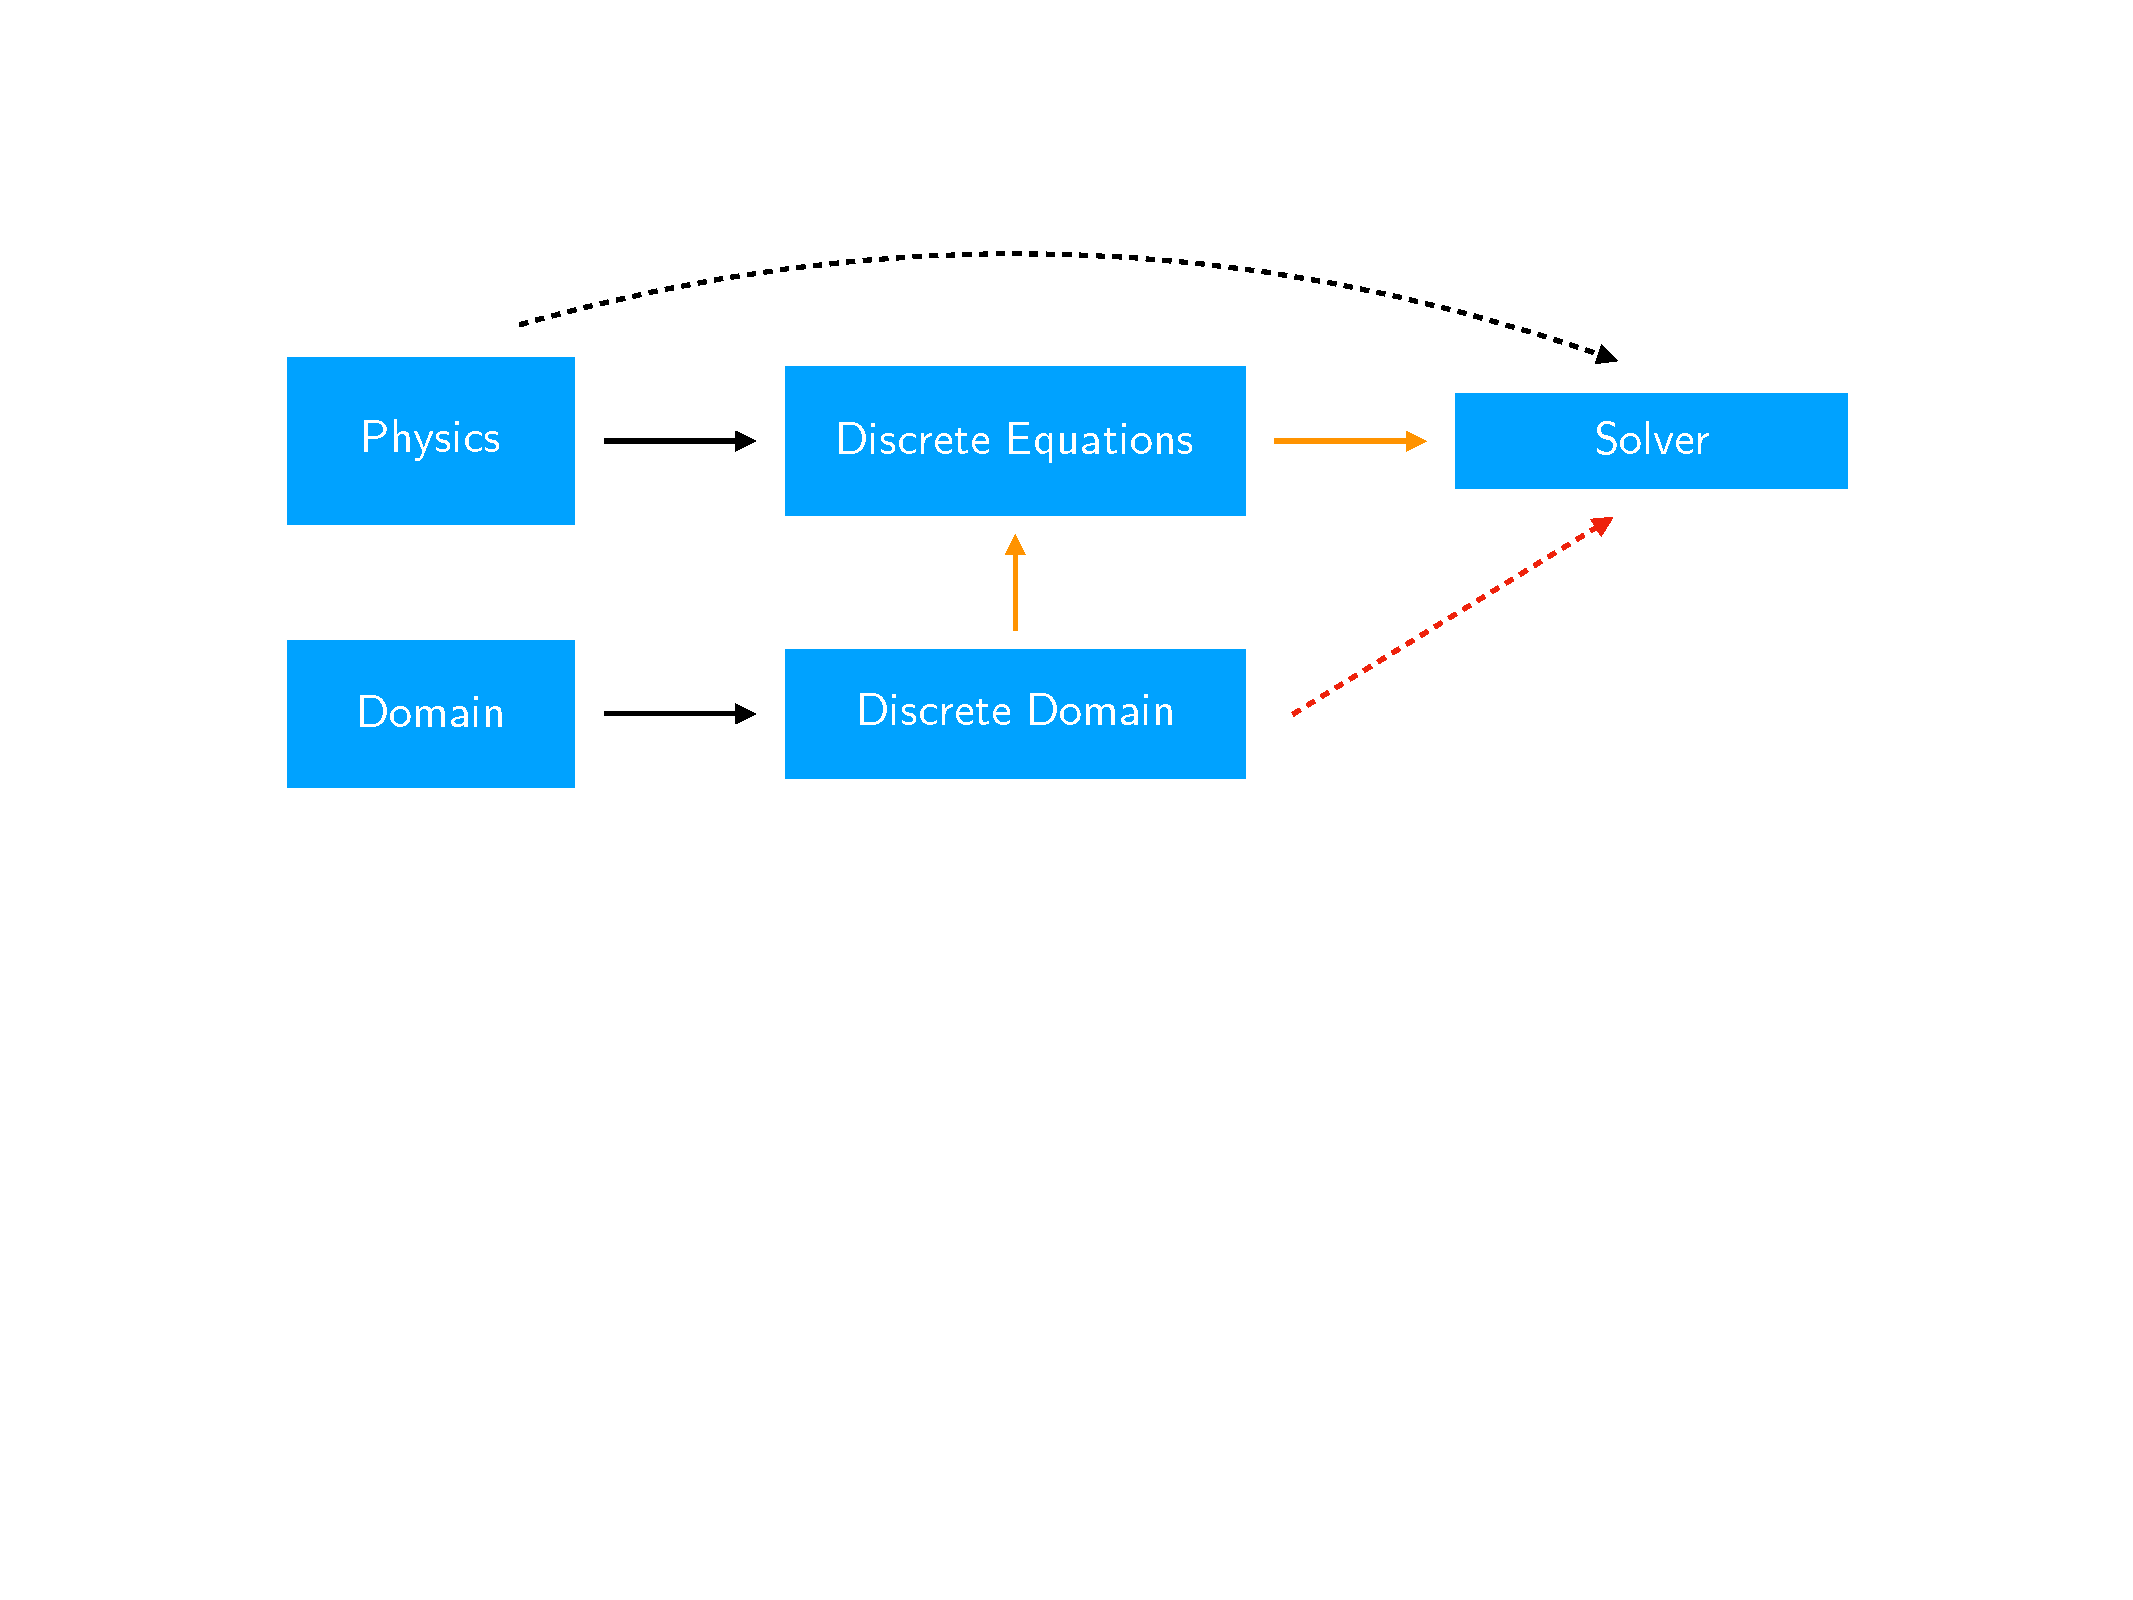
\includegraphics[width=0.8\textwidth]{images/need_for_dm.pdf}
  \begin{itemize}
    \item More information about the problem ("structure") can help solvers perform better
    \item Adding the dotted red line helps greatly when combined with the discrete equations (and the physics)
    \item Algebraic multigrid attempts to reconstruct this information from the discrete equations (the matrix)
  \end{itemize}
\end{frame}

%%%%%%%%%%%%%%%%%%%%%%%%%%%%%%%%%%%%%%%%%%%%%%%%%%%%%%%%%%%%%%%%%%%%%%%%%%%%%%%%
\begin{frame}[fragile]
  \frametitlelogo{What's in a \texttt{DM}?}
  A working definition of a \texttt{DM}:
\begin{center}
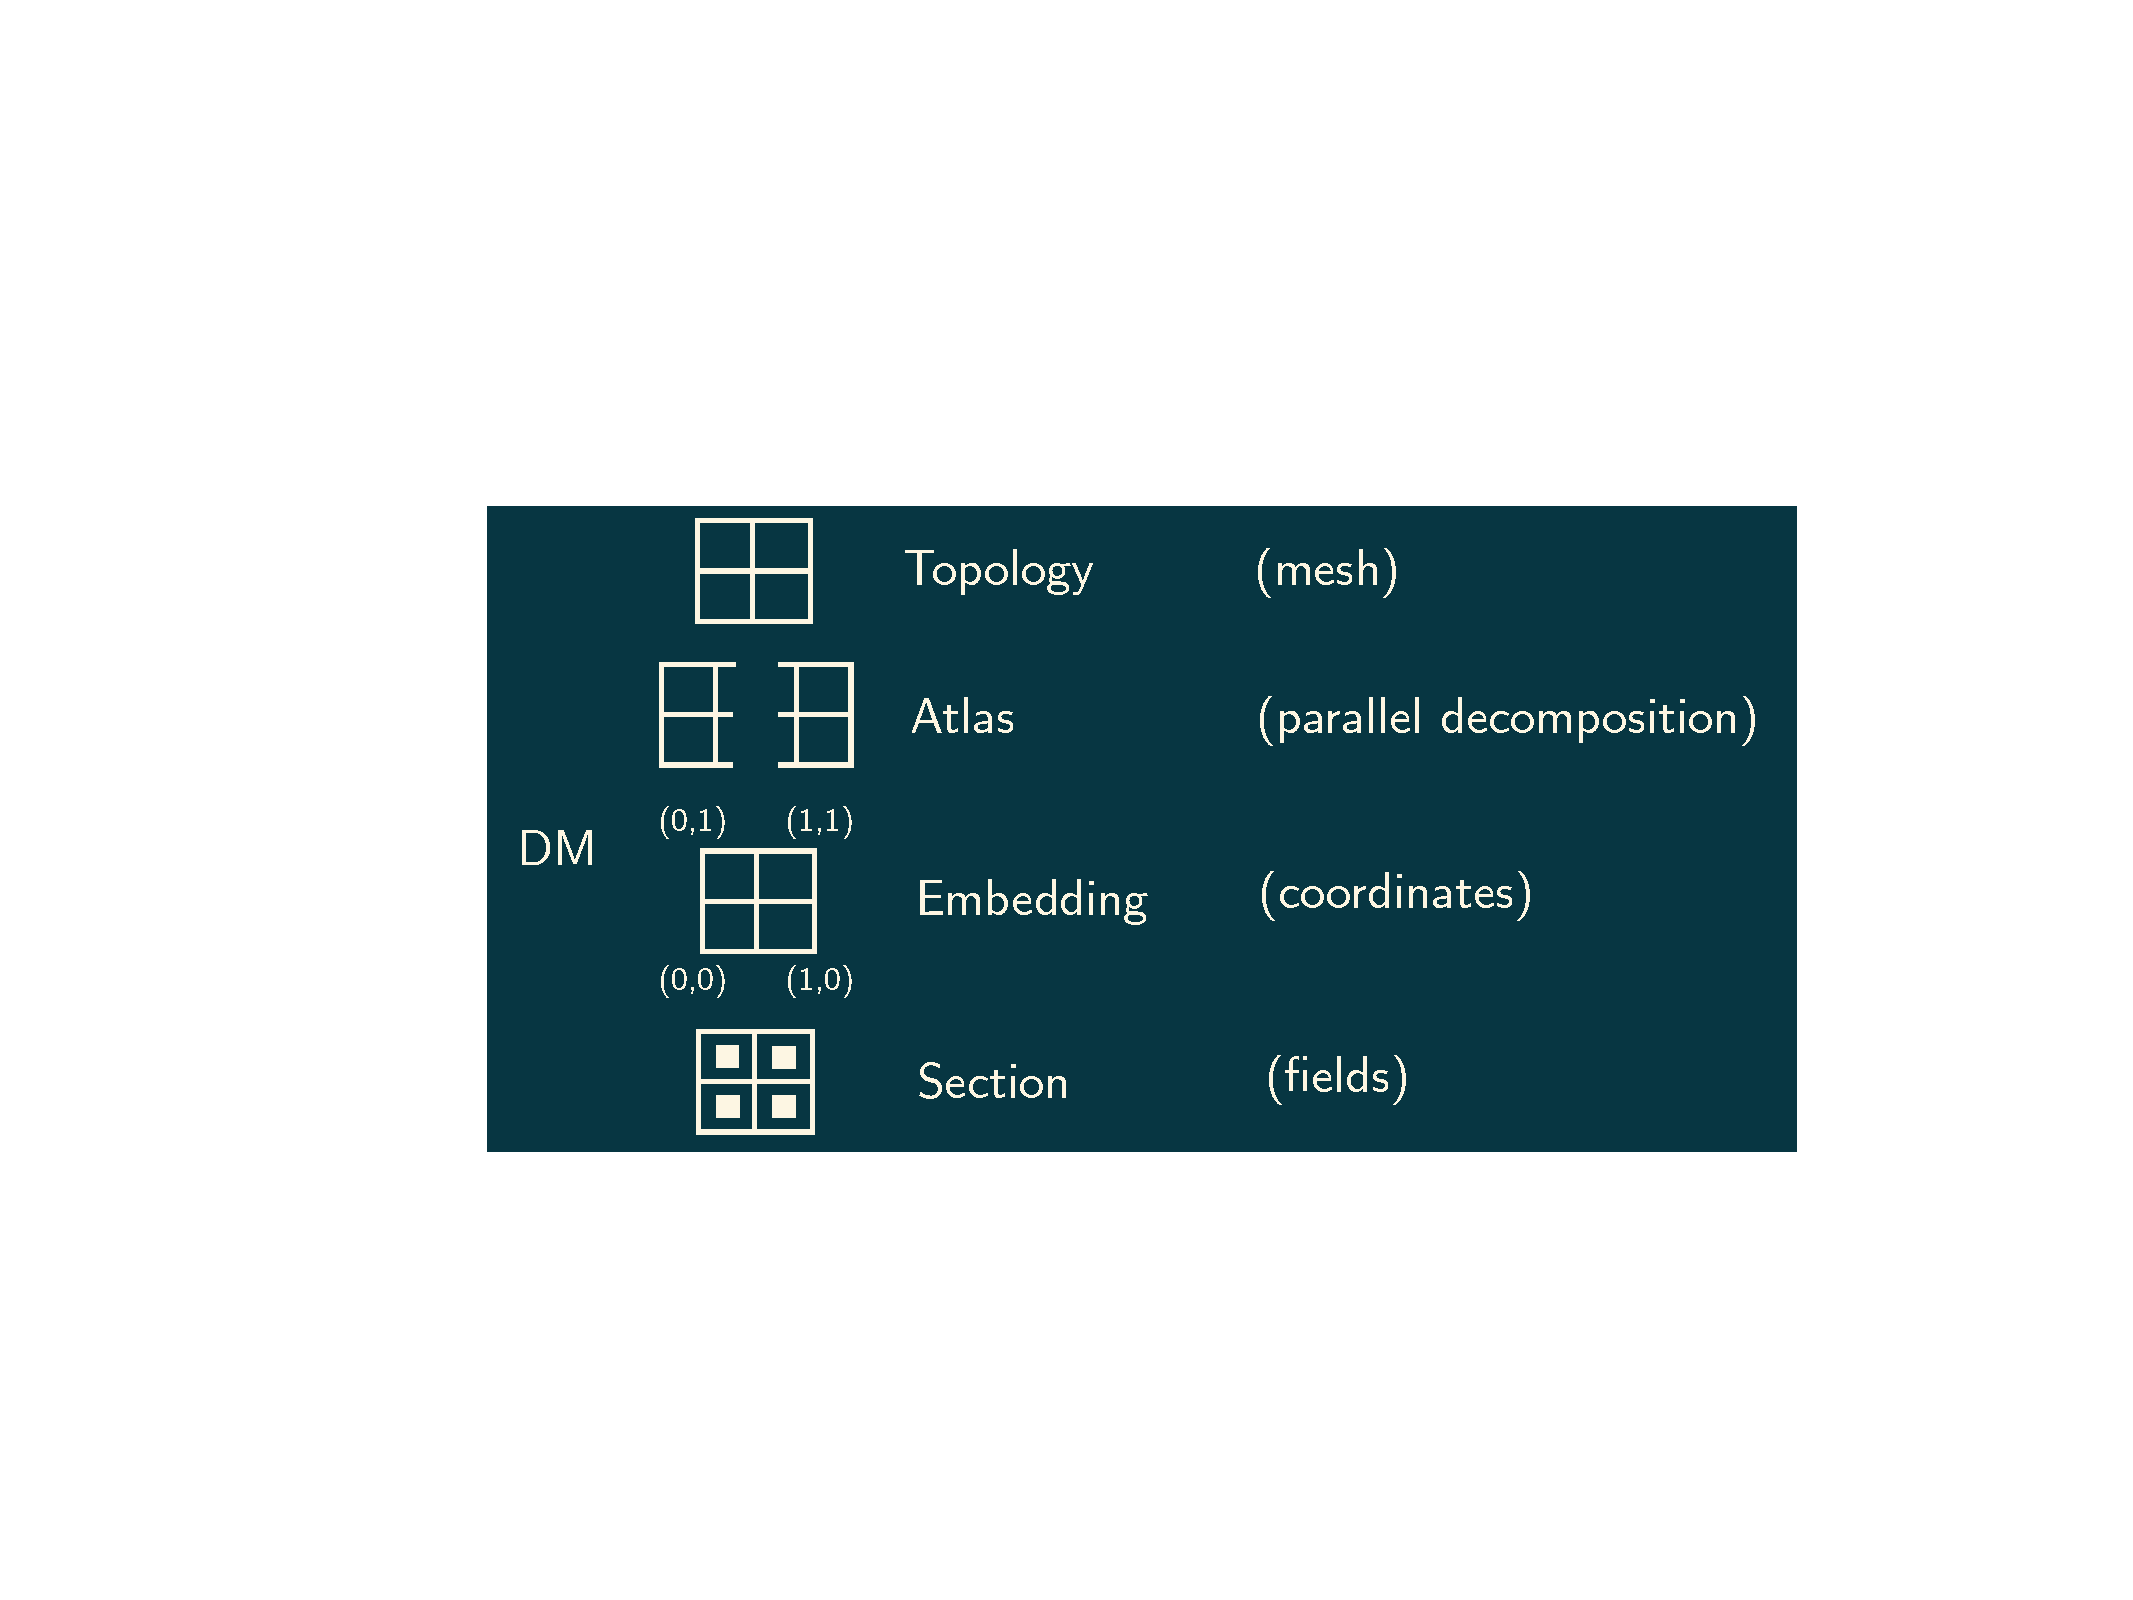
\includegraphics[width=\textwidth]{whatsadm_cut}
\end{center}
\begin{itemize}
  \item  Note: different sections (fields, data, ..) on the ``same domain'' require different \texttt{DM}s.
\end{itemize}
\end{frame}

%%%%%%%%%%%%%%%%%%%%%%%%%%%%%%%%%%%%%%%%%%%%%%%%%%%%%%%%%%%%%%%%%%%%%%%%%%%%%%%%
\begin{frame}[fragile]
  \frametitlelogo{Hands on: DMDA (parallel, regular grid)}
  \begin{itemize}
    \item When your problem is set up using a \lstinline{DM}, you can test, and hopefully use, advanced parallel solvers
  \item Let's experiment with the Poisson equation, using PETSc's default linear solver (robust, but not optimal)
\begin{lstlisting}[language=bash,basicstyle=\scriptsize\ttfamily]
  # Define PETSC_DIR and PETSC_ARCH
  cd $PETSC_DIR/src/ksp/ksp/examples/tutorials
  make ex50
  ./ex50 -da_refine 5 -ksp_view -ksp_monitor \
    -ksp_converged_reason
  \end{lstlisting}
  \item We can do better with algebraic multigrid
\begin{lstlisting}[language=bash,basicstyle=\scriptsize\ttfamily]
  ./ex50 -da_refine 5 -ksp_view -ksp_monitor \
    -ksp_converged_reason -pc_type gamg
  \end{lstlisting}
  \item And even better with geometric multigrid:
\begin{lstlisting}[language=bash,basicstyle=\scriptsize\ttfamily]
  ./ex50 -da_refine 5 -ksp_view -ksp_monitor \
    -ksp_converged_reason -pc_type mg -pc_mg_levels 5 \
    -pc_mg_type full  # add -log_view for timing!
  \end{lstlisting}
  \item How did it work? The DM helped create the multigrid components!
  \end{itemize}
\end{frame}


%%%%%%%%%%%%%%%%%%%%%%%%%%%%%%%%%%%%%%%%%%%%%%%%%%%%%%%%%%%%%%%%%%%%%%%%%%%%%%%%
\begin{frame}[fragile]
\frametitle{DMStag}
  \begin{itemize}
  \item A generalization of DMDA for staggered grids
  \item Why not just use DMDA(s) for staggered grid problems?
    \begin{itemize}
    \item Must either use dummy/ghost points with a multi-dof collocated grid,  plus extra indexing (I3ELVIS), or..
    \item Multiple DMDAs, plus extra indexing (LaMEM)
    \item Difficult to present a uniform interface to solvers
    \end{itemize}
  \end{itemize}
  \begin{center}
  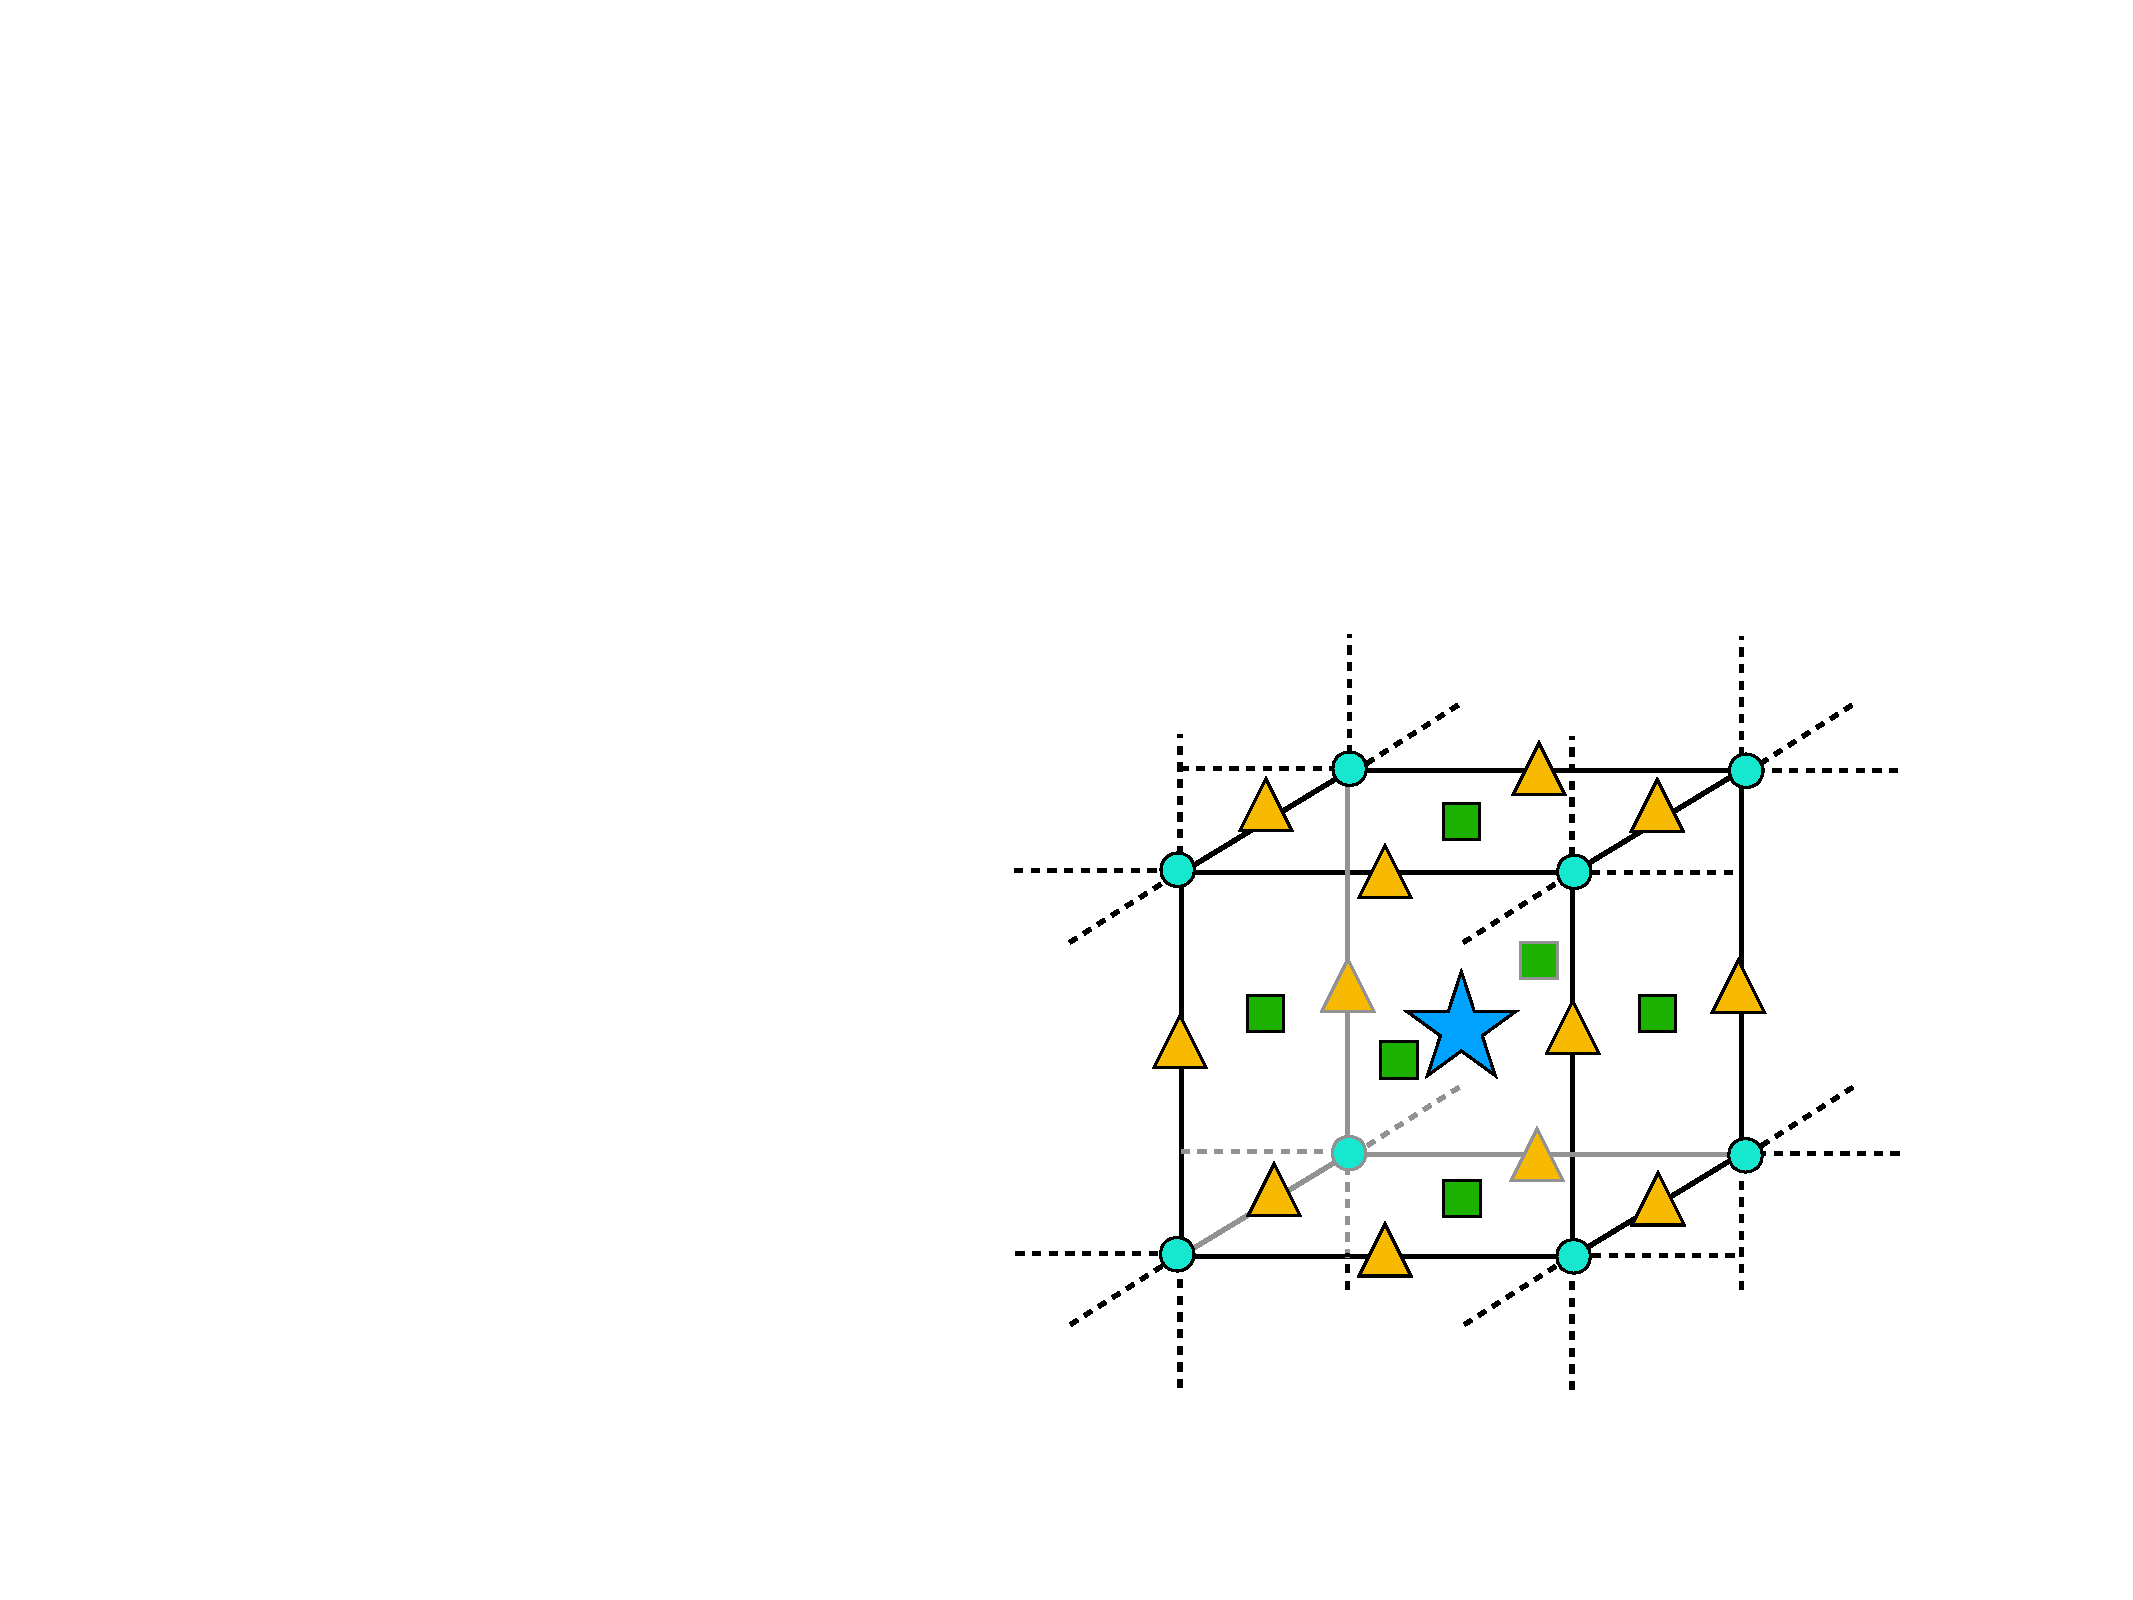
\includegraphics[width=0.4\textwidth]{images/3d_grid_cartoon.pdf}
  \end{center}
\end{frame}

%%%%%%%%%%%%%%%%%%%%%%%%%%%%%%%%%%%%%%%%%%%%%%%%%%%%%%%%%%%%%%%%%%%%%%%%%%%%%%%%
%%%%%%%%%%%%%%%%%%%%%%%%%%%%%%%%%%%%%%%%%%%%%%%%%%%%%%%%%%%%%%%%%%%%%%%%%%%%%%%%
\section{Tutorial Example}

%%%%%%%%%%%%%%%%%%%%%%%%%%%%%%%%%%%%%%%%%%%%%%%%%%%%%%%%%%%%%%%%%%%%%%%%%%%%%%%%
\begin{frame}[fragile]
\frametitle{DMStag tutorial \texttt{ex6}: Seismic wave propagation}
\begin{itemize}
\item We'll work with an existing example, and use it to demonstrate the features of DMStag
\item With each topic, we'll modify the example to do something new
\item Disclaimer: I am not a seismologist!
\end{itemize}
\begin{center}

\includegraphics[width=0.4\textwidth]{images/dmstag_ex6_yvel_485.png}
\end{center}
\end{frame}

\begin{frame}[fragile]
\frametitle{Example Code}
  \begin{itemize}
    \item The code is found at \lstinline{$PETSC_DIR/src/dm/impls/stag/examples/tutorials/ex6.c}
      \item It shows an example of taking a published staggered-grid algorithm and implementing it
      \item The application is seismic wave propagation, from Virieux's 1986 paper \footfullcite{Virieux1986} (Thanks to B. Kaus for suggesting this as an example)
  \end{itemize}
  \begin{center}
  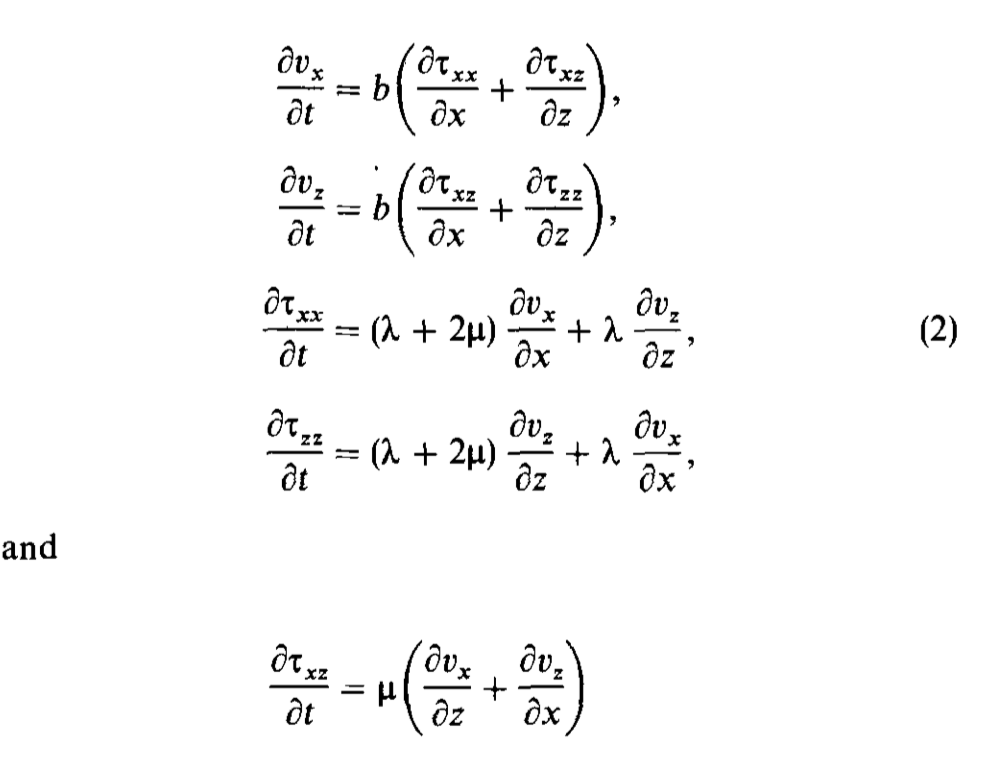
\includegraphics[width=0.4\textwidth]{images/virieux1986_eq2.png}
  \end{center}
\end{frame}

\begin{frame}[fragile]
\frametitle{Example Code}
  \begin{minipage}{0.54\textwidth}
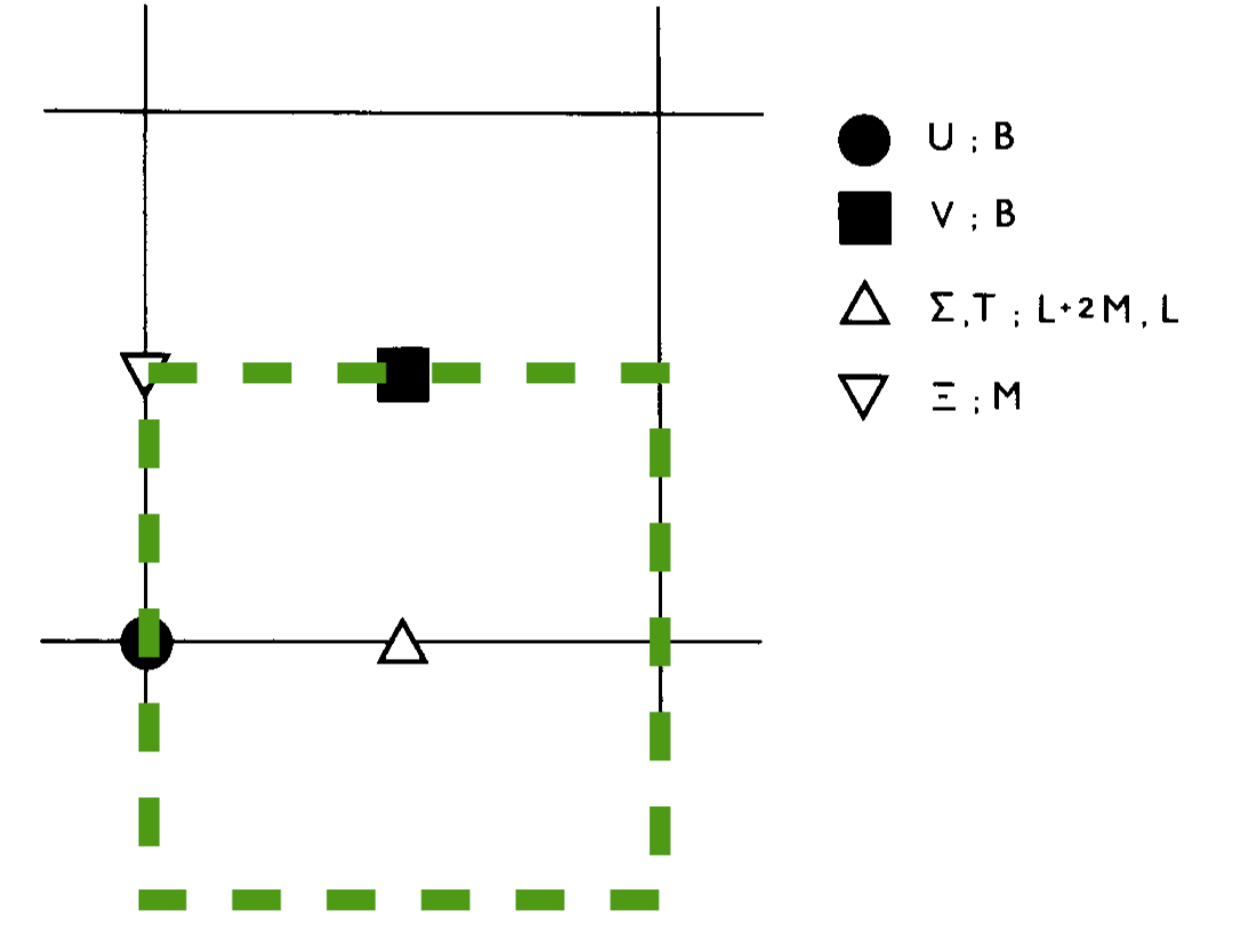
\includegraphics[width=\textwidth]{images/virieux1986_fig1_part1_mod.png}
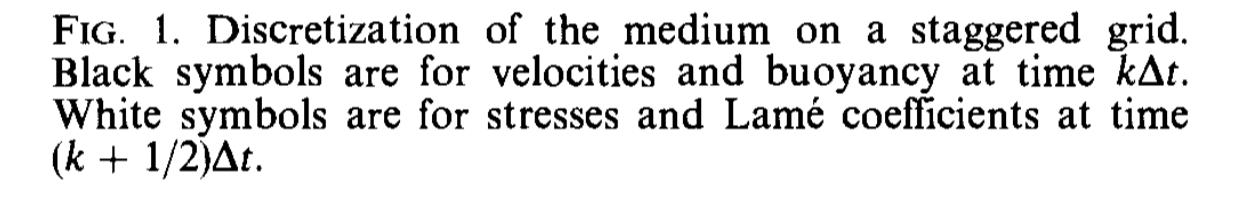
\includegraphics[width=\textwidth]{images/virieux1986_fig1_part2.png}
    {\tiny(modified to add a more natural control volume)}
  \end{minipage}
  \begin{minipage}{0.44\textwidth}
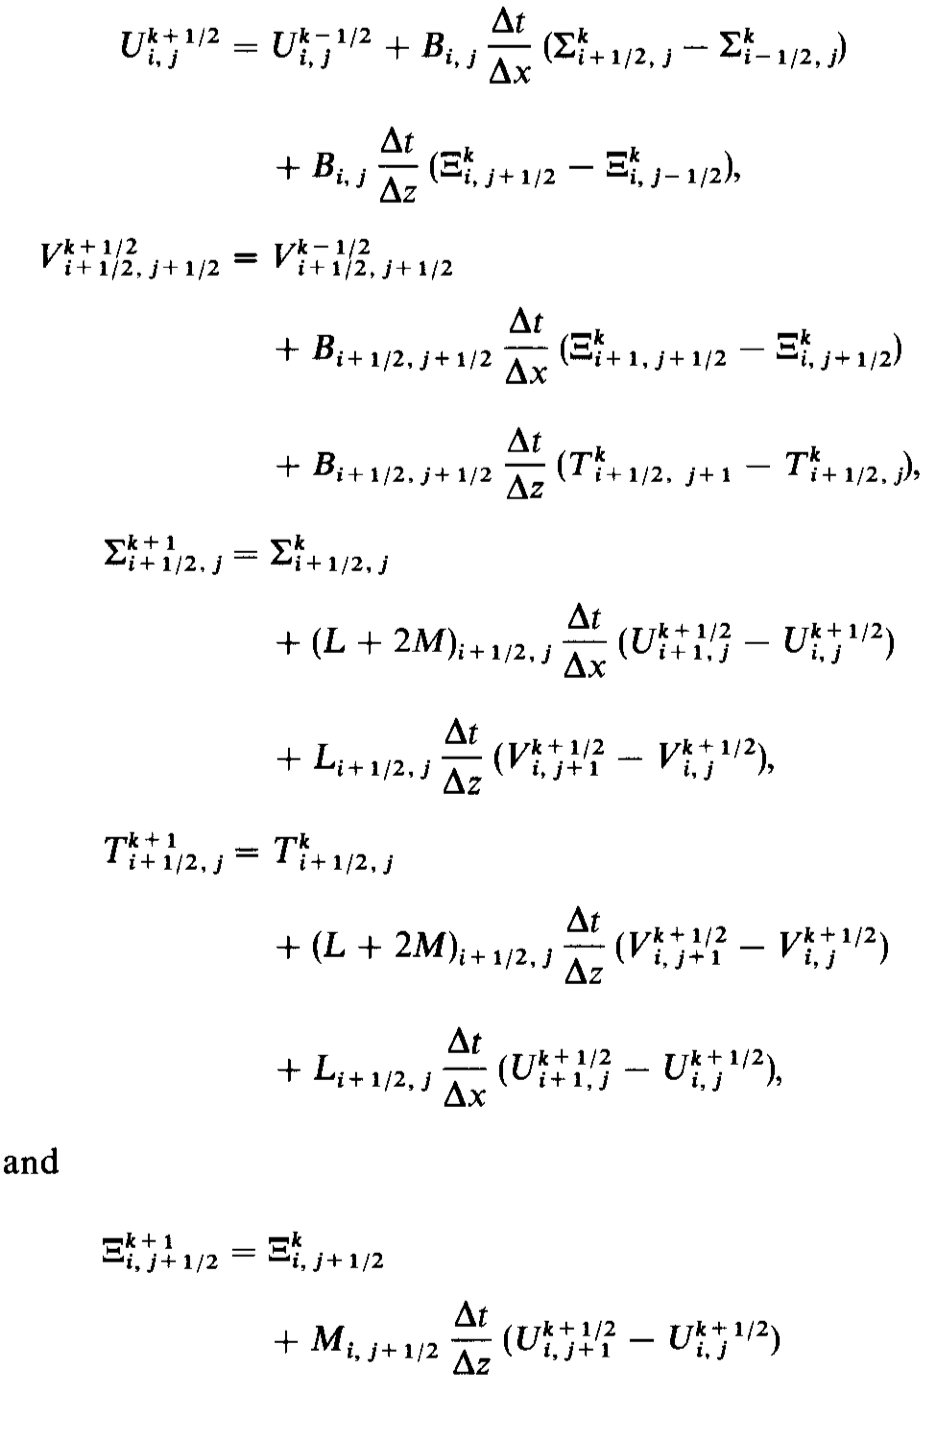
\includegraphics[width=\textwidth]{images/virieux1986_eq5_part1.png}
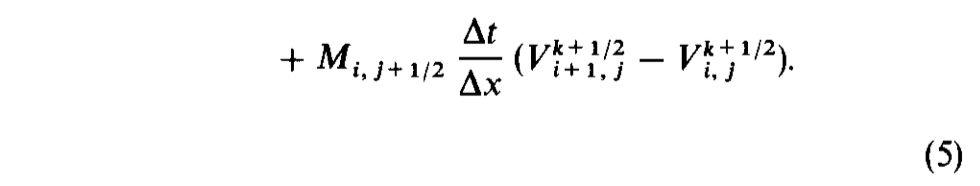
\includegraphics[width=\textwidth]{images/virieux1986_eq5_part2.png}
  \end{minipage}
\end{frame}

\begin{frame}[fragile]
\frametitle{Example Code}
  To run the code, you must first have a working build of PETSc (which
  you hopefully already do!)
\begin{lstlisting}[language=bash,basicstyle=\scriptsize\ttfamily]
  export PETSC_DIR=xxx
  export PETSC_ARCH=yyy
  cd $PETSC_DIR/src/dm/impls/stag/examples/tutorials/ex6.c
  make ex6
  rm -f *.vtr && $PETSC_DIR/$PETSC_ARCH/bin/mpiexec -np 4 ./ex6
\end{lstlisting}
  Examine the resulting \texttt{.vtr} files in Paraview
\end{frame}

%%%%%%%%%%%%%%%%%%%%%%%%%%%%%%%%%%%%%%%%%%%%%%%%%%%%%%%%%%%%%%%%%%%%%%%%%%%%%%%%
%%%%%%%%%%%%%%%%%%%%%%%%%%%%%%%%%%%%%%%%%%%%%%%%%%%%%%%%%%%%%%%%%%%%%%%%%%%%%%%%
\section{Creation and Setup}

%%%%%%%%%%%%%%%%%%%%%%%%%%%%%%%%%%%%%%%%%%%%%%%%%%%%%%%%%%%%%%%%%%%%%%%%%%%%%%%%
\begin{frame}[fragile]
\frametitle{Creation}
High-level functions create new DMStag objects.
\begin{lstlisting}[language=C,basicstyle=\scriptsize\ttfamily]
ierr = DMStagCreate2d(
  PETSC_COMM_WORLD,
  DM_BOUNDARY_NONE,DM_BOUNDARY_NONE, /* Boundary types          */
  7,9,                               /* Global sizes            */
  PETSC_DECIDE,PETSC_DECIDE,         /* Local sizes             */
  dof0,dof1,dof2,                    /* dof per stratum:
                                          0: vertices
                                          1: edges
                                          2: faces
                                          3: hexes              */
  DMSTAG_GHOST_STENCIL_STAR,         /* Elementwise ghosting    */
  stencilWidth,                      /* Elementwise ghost width */
  NULL,NULL,                         /* explicit decomposition  */
  &my_dmstag
);CHKERRQ(ierr);
\end{lstlisting}

  {\small
  Manual pages for all DMStag functions can be found on the web
  \begin{itemize}
      \item Release:
        {\tiny\href{https://www.mcs.anl.gov/petsc/petsc-current/docs/manualpages/DMSTAG/index.html}{https://www.mcs.anl.gov/petsc/petsc-current/docs/manualpages/DMSTAG/index.html}}
\item Development (latest):
  {\tiny
      \href{https://www.mcs.anl.gov/petsc/petsc-dev/docs/manualpages/DMSTAG/index.html}{https://www.mcs.anl.gov/petsc/petsc-dev/docs/manualpages/DMSTAG/index.html}}
  \end{itemize}
  }
\end{frame}

%%%%%%%%%%%%%%%%%%%%%%%%%%%%%%%%%%%%%%%%%%%%%%%%%%%%%%%%%%%%%%%%%%%%%%%%%%%%%%%%
\begin{frame}[fragile]
\frametitle{Creation: Exercise}
  The call to \lstinline{DMSetFromOptions()} allows many options to be specified with command line flags,
  and we also add our own.
  \begin{itemize}
  \item From the command line,
    \begin{itemize}
      \item Get short (\lstinline{-help intro}) or long (\lstinline{-help}) sets of options
      \item more timesteps  (\lstinline{-nsteps})
      \item A different grid size (\lstinline{stag_grid_x 50 -stag_grid_y 50}
      \item Try different parallel decompositions (\lstinline{-stag_ranks_x 1})
      \item Investigate how performance changes (\lstinline{-log_view})
    \end{itemize}
  \end{itemize}
\end{frame}

%%%%%%%%%%%%%%%%%%%%%%%%%%%%%%%%%%%%%%%%%%%%%%%%%%%%%%%%%%%%%%%%%%%%%%%%%%%%%%%%
%%%%%%%%%%%%%%%%%%%%%%%%%%%%%%%%%%%%%%%%%%%%%%%%%%%%%%%%%%%%%%%%%%%%%%%%%%%%%%%%
\section{Local and Global Representations}

%%%%%%%%%%%%%%%%%%%%%%%%%%%%%%%%%%%%%%%%%%%%%%%%%%%%%%%%%%%%%%%%%%%%%%%%%%%%%%%%
\begin{frame}[fragile]
  \frametitlelogo{\texttt{DMStag} Local-Global Wrinkles}
\begin{itemize}
  \item The local representation is uniformly-blocked, but has ``dummy'' points
  \item The global representation is not uniformly-blocked, but only contains dof corresponding to actual cells in the cell complex
  \item ``Think globally, act locally''
  \item Based on the experience of users with \PETSc{}'s existing local-global paradigm, performance bottlenecks related to redundant local-global information aren't as common as one might expect, but an available future optimization is implementing \lstinline{DMLocalToLocal()} for \texttt{DMStag}.
\end{itemize}
\end{frame}



%%%%%%%%%%%%%%%%%%%%%%%%%%%%%%%%%%%%%%%%%%%%%%%%%%%%%%%%%%%%%%%%%%%%%%%%%%%%%%%%
\begin{frame}[fragile]
  \frametitlelogo{DMStag Natural (user-facing) indexing}
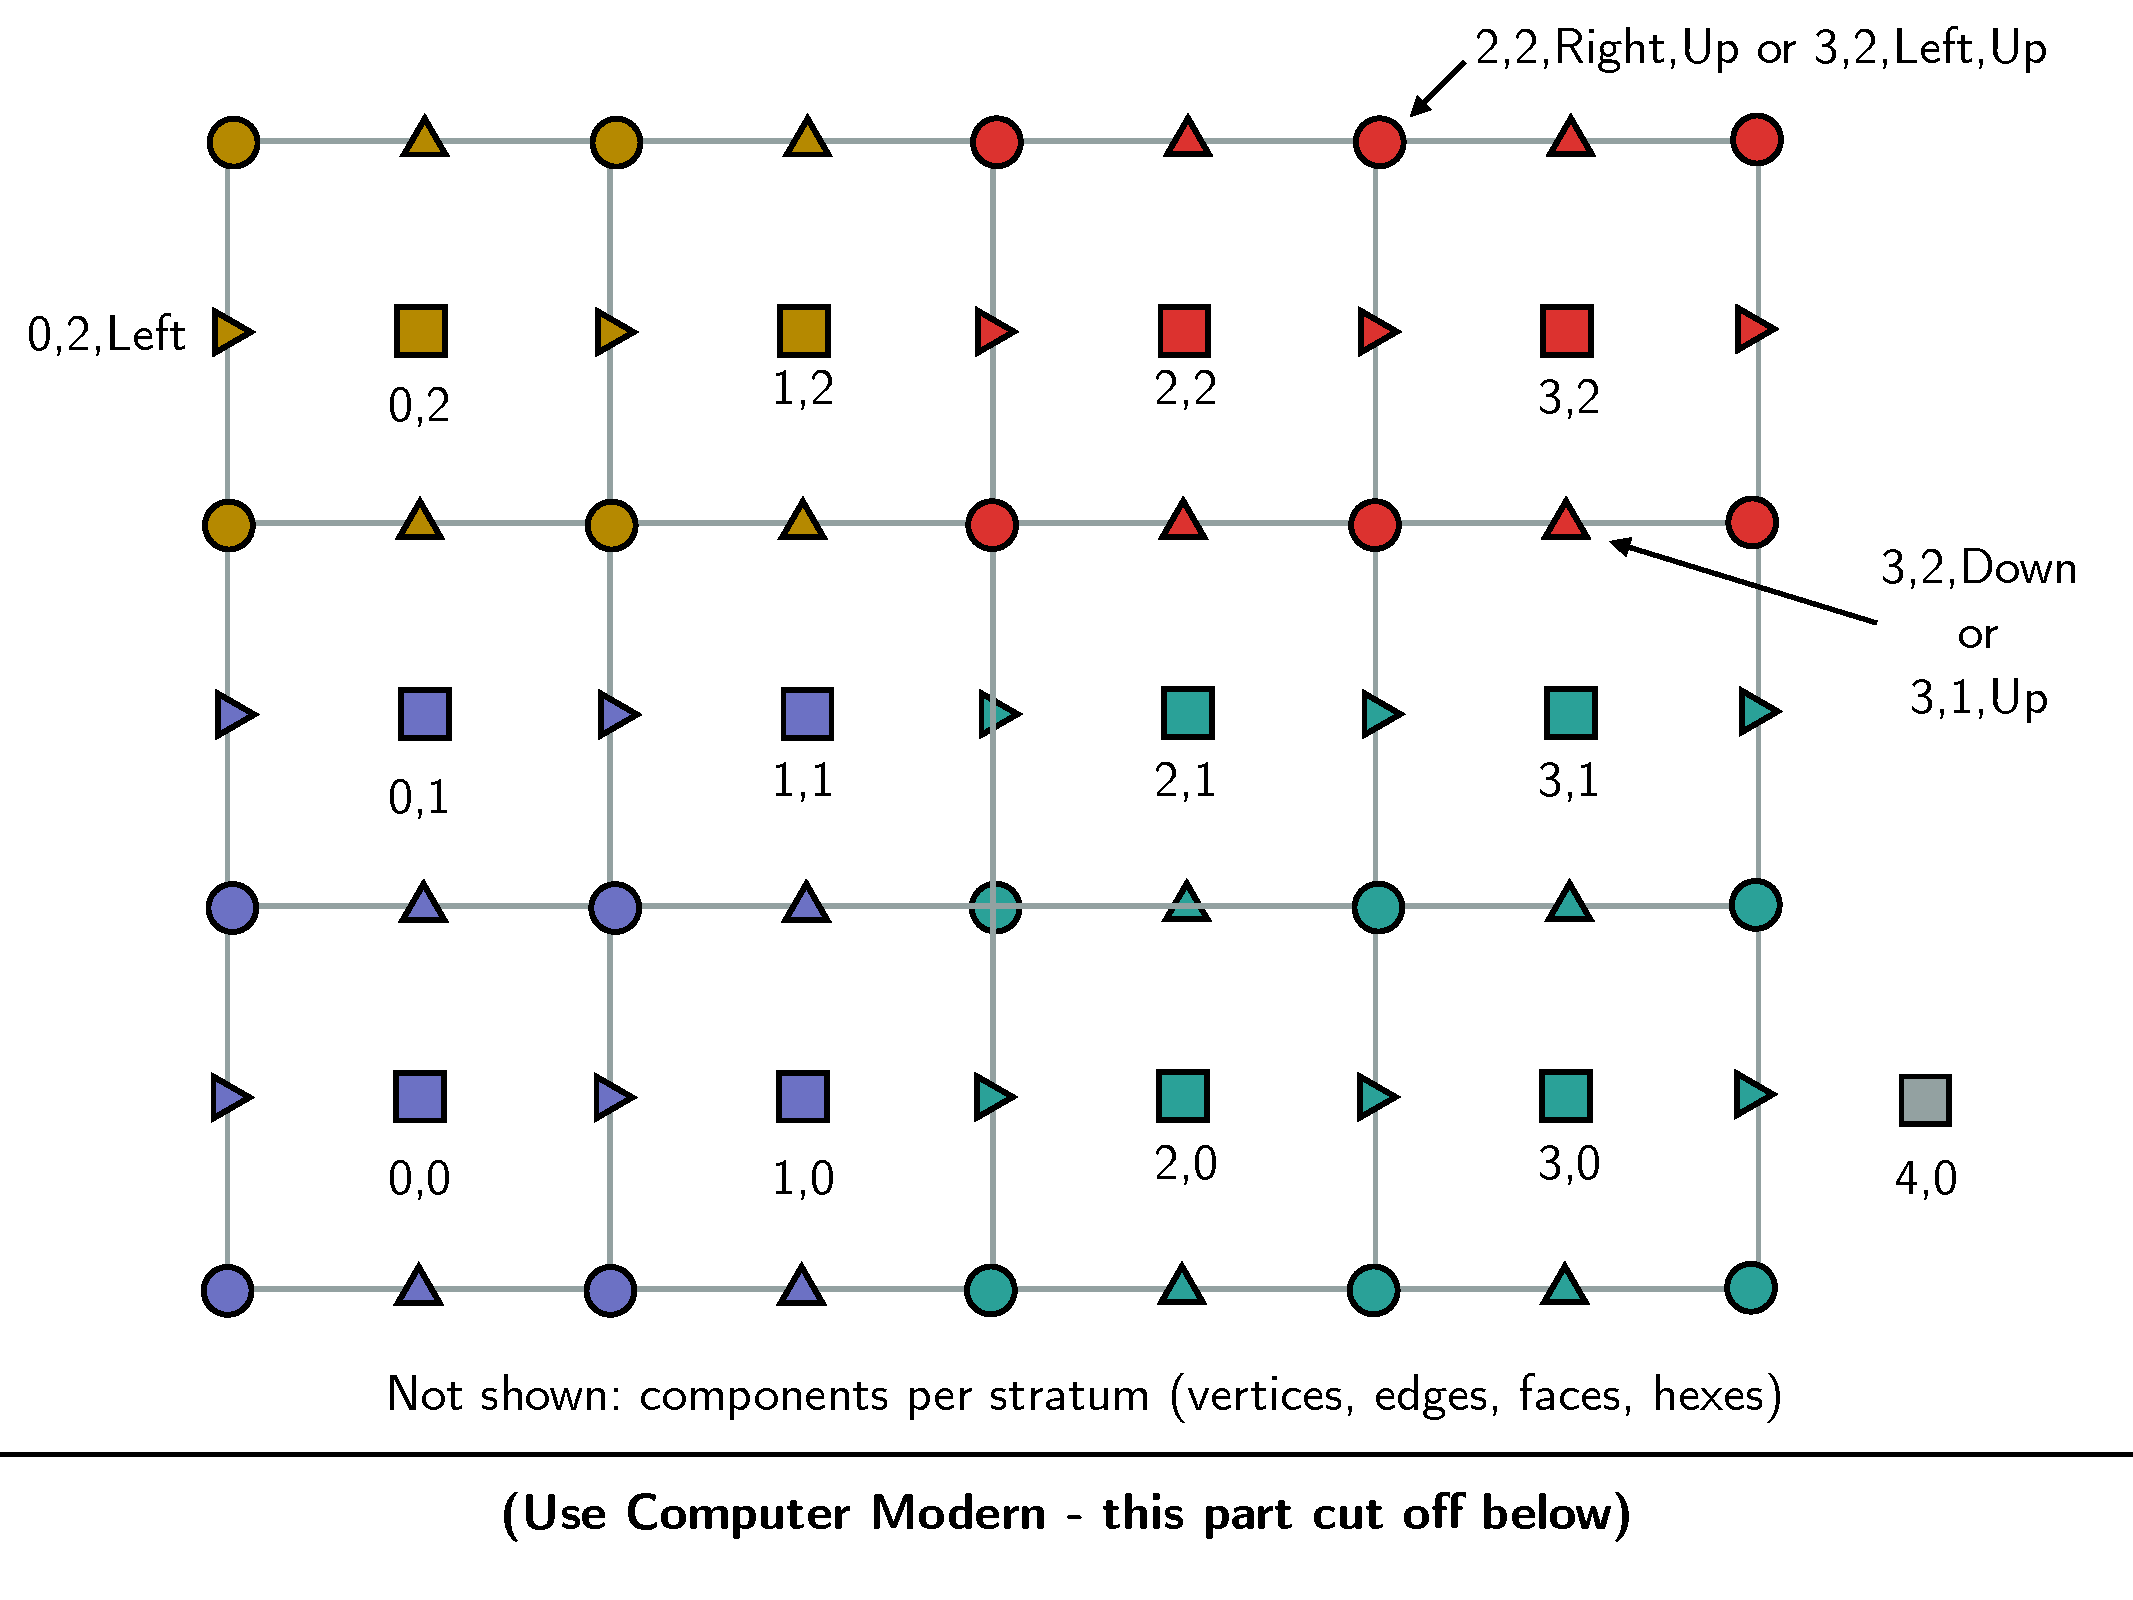
\includegraphics[width=\textwidth]{natural_numbering}
\end{frame}

%%%%%%%%%%%%%%%%%%%%%%%%%%%%%%%%%%%%%%%%%%%%%%%%%%%%%%%%%%%%%%%%%%%%%%%%%%%%%%%%
\begin{frame}[fragile]
\frametitlelogo{Internal Local and Global Indexing (1 dof/stratum)}
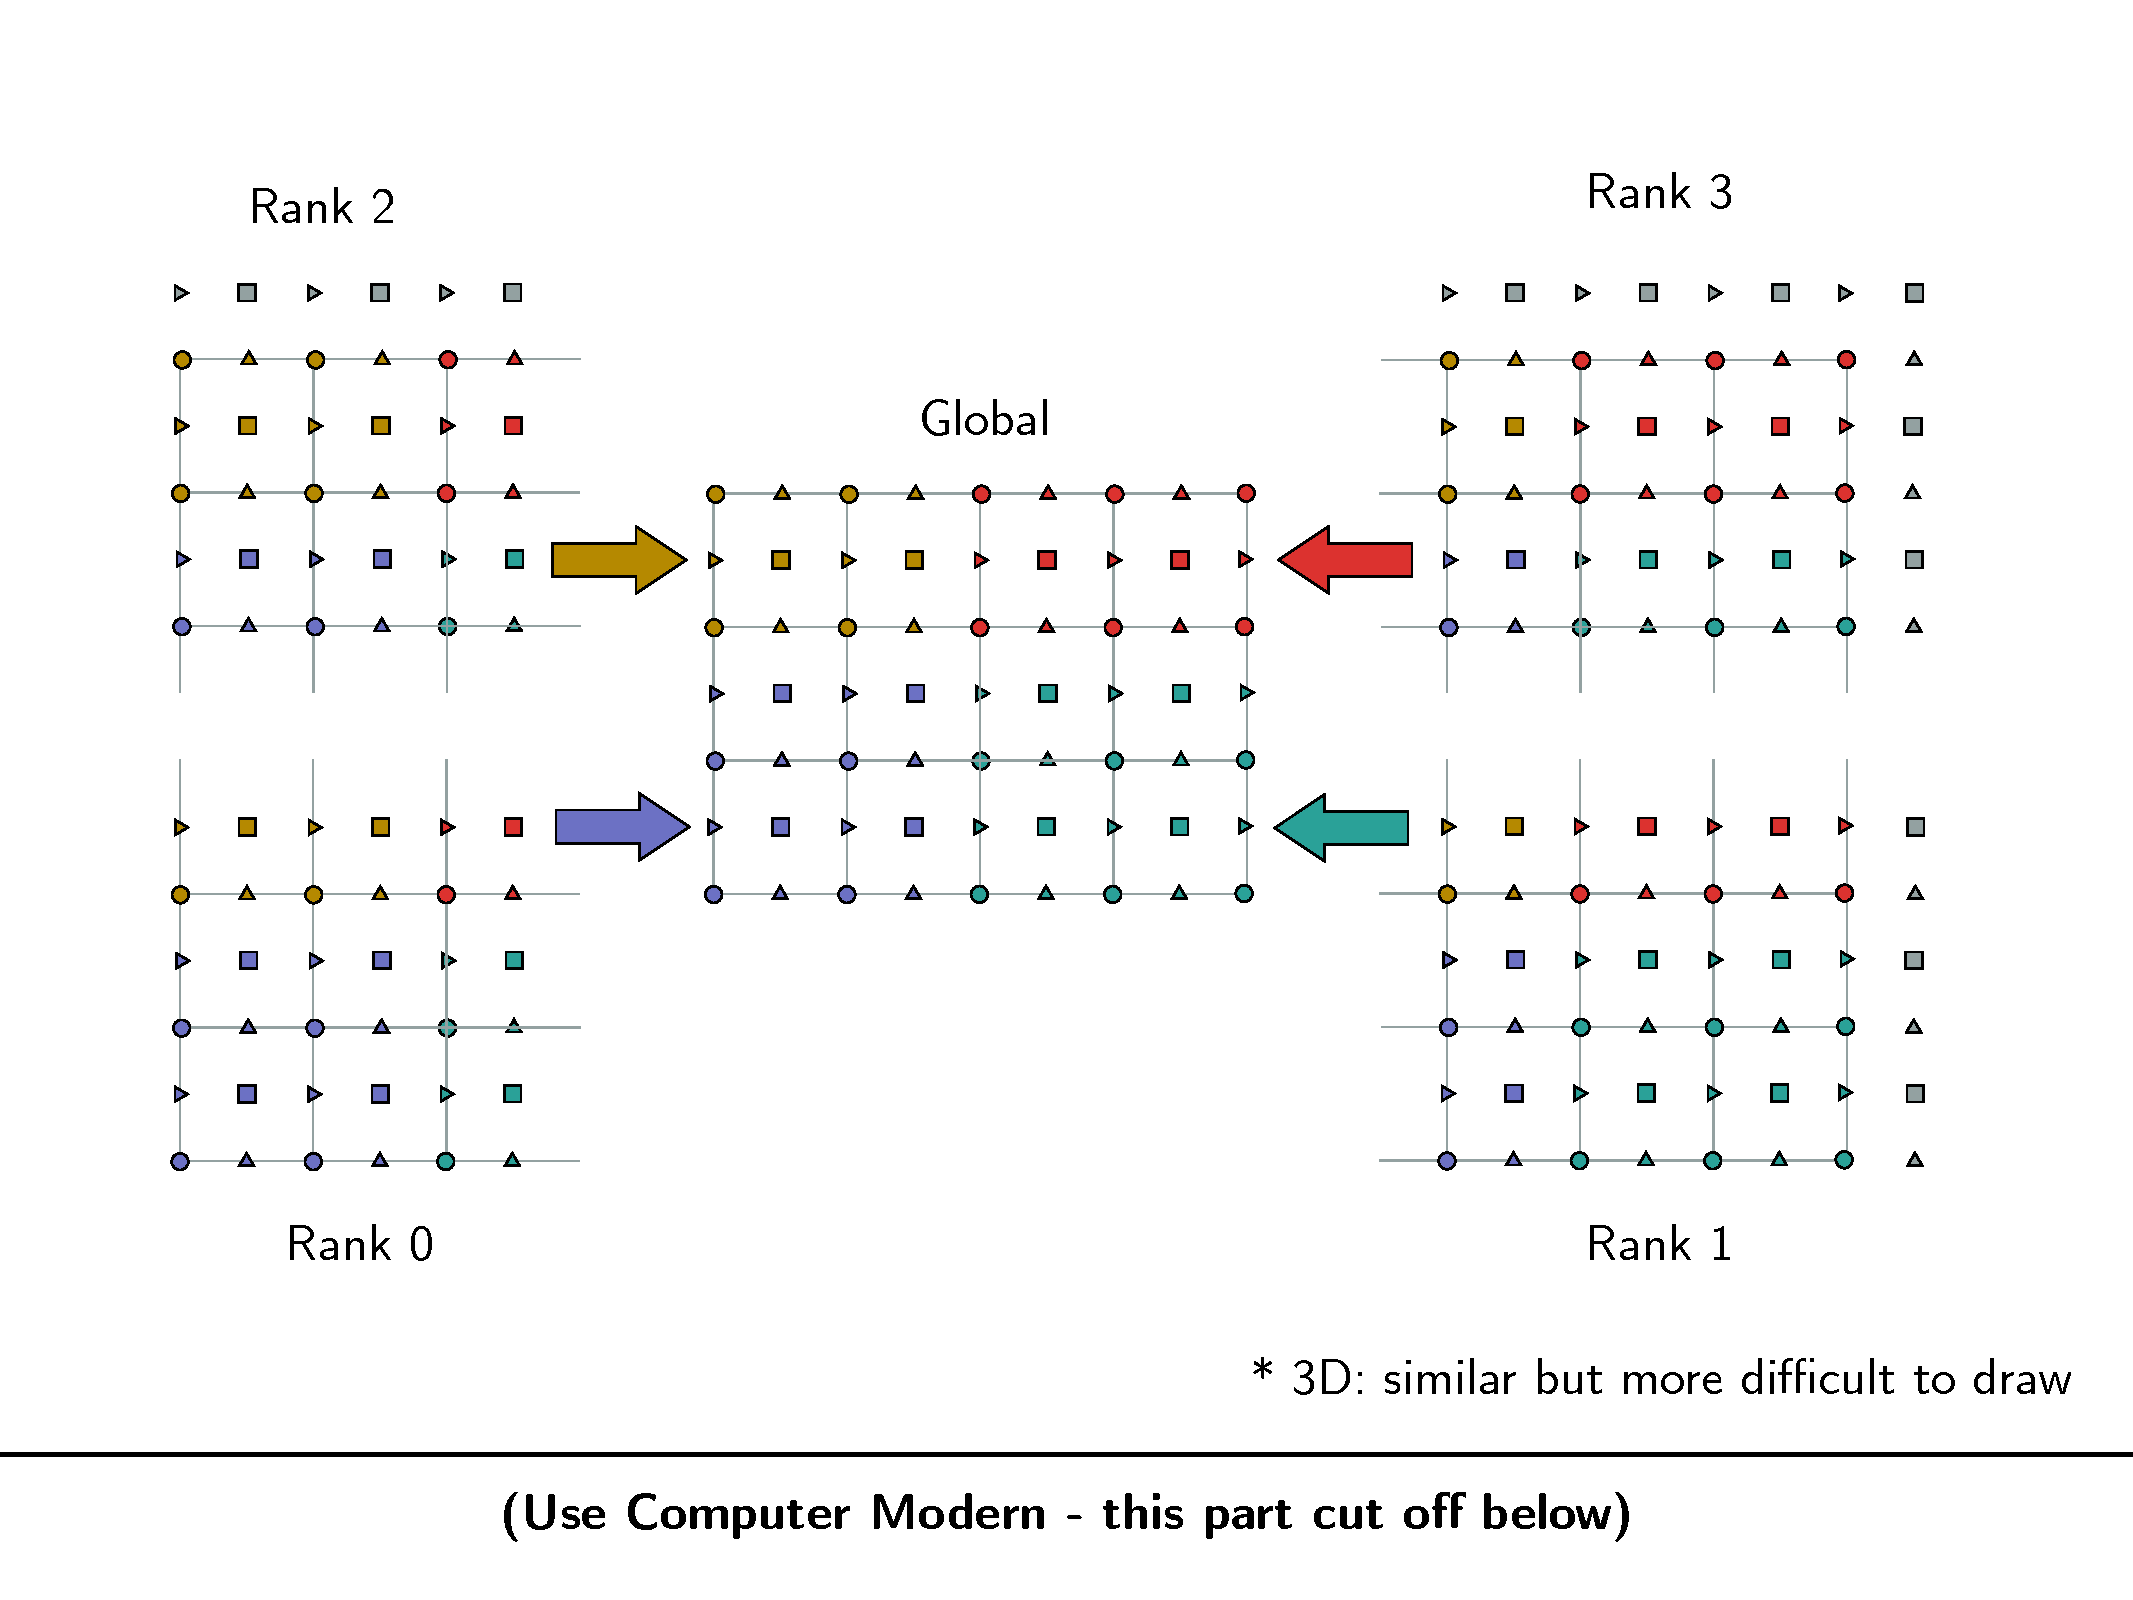
\includegraphics[width=\textwidth]{local_global}
\end{frame}

%%%%%%%%%%%%%%%%%%%%%%%%%%%%%%%%%%%%%%%%%%%%%%%%%%%%%%%%%%%%%%%%%%%%%%%%%%%%%%%%
\begin{frame}[fragile]
\frametitlelogo{Internal Local and Global Indexing (1 dof/stratum)}
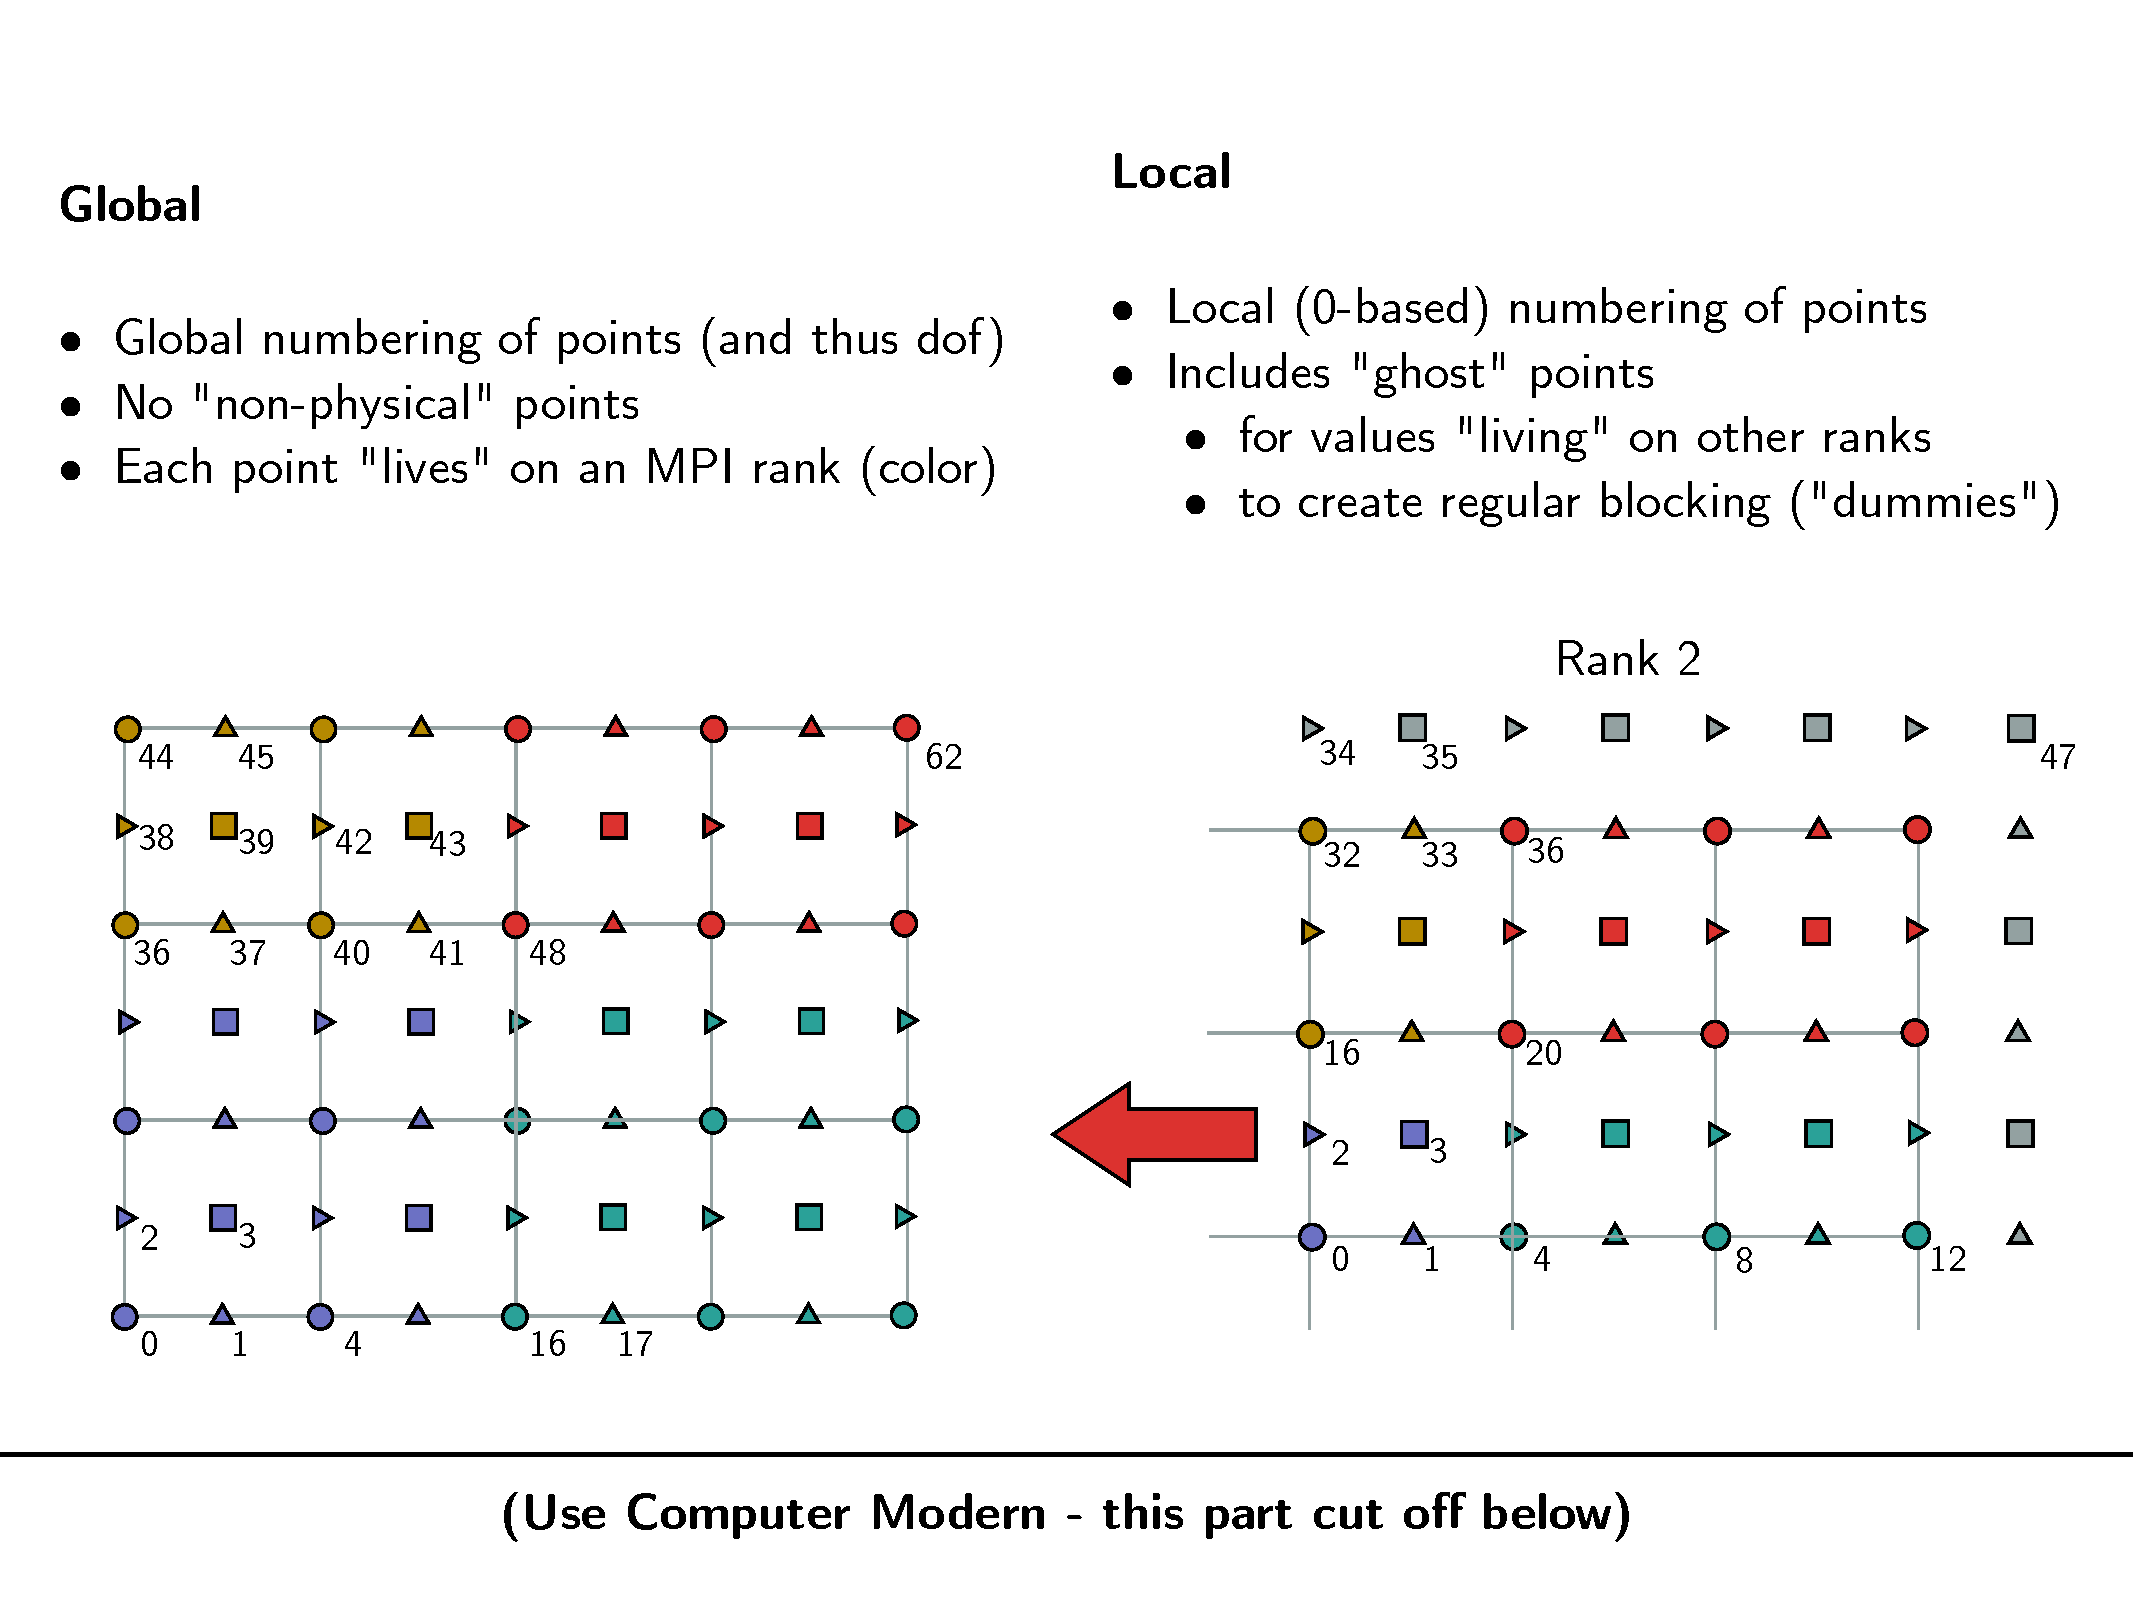
\includegraphics[width=\textwidth]{global_local_numbers}
\end{frame}

%%%%%%%%%%%%%%%%%%%%%%%%%%%%%%%%%%%%%%%%%%%%%%%%%%%%%%%%%%%%%%%%%%%%%%%%%%%%%%%%
\begin{frame}[fragile]
\frametitle{Hands on: Local and Global Representations}
Examine the raw data in the local and global representations. How are the sizes and entries different?
\begin{itemize}
\item Run a single timestep, for a small problem
\begin{lstlisting}[language=C,basicstyle=\scriptsize\ttfamily]
./ex6 -nsteps 1 -stag_grid_x 4 -stag_grid_z 4
\end{lstlisting}
\item View a local coefficient vector by adding e.g.
\begin{lstlisting}[language=C,basicstyle=\scriptsize\ttfamily]
ierr = VecView(lame_local,PETSC_VIEWER_STDOUT_WORLD);CHKERRQ(ierr);
\end{lstlisting}
\item View the global coefficient vector by adding e.g.
\begin{lstlisting}[language=C,basicstyle=\scriptsize\ttfamily]
ierr = VecView(lame_local,PETSC_VIEWER_STDOUT_WORLD);CHKERRQ(ierr);
\end{lstlisting}
\item Repeat in parallel. Use the write \texttt{mpiexec}. If you used \texttt{--download-mpich}, you can use
\begin{lstlisting}[language=C,basicstyle=\scriptsize\ttfamily]
$PETSC_DIR/$PETSC_ARCH/bin/mpiexec -np 4 ./ex6
\end{lstlisting}
\end{itemize}
  Bonus: try to do the same without changing the code, using a debugger (\texttt{gdb} or \texttt{lldb}) and calling \lstinline{VecView(vec,0)} directly.
\end{frame}

%%%%%%%%%%%%%%%%%%%%%%%%%%%%%%%%%%%%%%%%%%%%%%%%%%%%%%%%%%%%%%%%%%%%%%%%%%%%%%%%
%%%%%%%%%%%%%%%%%%%%%%%%%%%%%%%%%%%%%%%%%%%%%%%%%%%%%%%%%%%%%%%%%%%%%%%%%%%%%%%%
\section{Working with arrays}

%%%%%%%%%%%%%%%%%%%%%%%%%%%%%%%%%%%%%%%%%%%%%%%%%%%%%%%%%%%%%%%%%%%%%%%%%%%%%%%%
\begin{frame}[fragile]
\frametitlelogo{Easier indexing with stencils!}
\begin{itemize}
\item Key feature in \texttt{DMStag} : \lstinline{DMStagStencil} (akin to \lstinline{MatStencil})
\item Language like ``The edge above element $(i,j)$'' better than raw indices.
\item It simply holds 5 integers: which element, which point, which dof.
\begin{lstlisting}[language=C]
typedef struct {
  DMStagStencilLocation loc; /* enum */
  PetscInt              i,j,k,c;
} DMStagStencil;
\end{lstlisting}
\item API uses these to translate between global element numbers/locations/components
and local indices, for both vectors and matrices.
\begin{lstlisting}[language=C]
PetscErrorCode DMStagVecGetValuesStencil(
                 DM dm,Vec vec, PetscInt n,
                 const DMStagStencil* pos,
                 PetscScalar*);
\end{lstlisting}
\end{itemize}
\end{frame}

%%%%%%%%%%%%%%%%%%%%%%%%%%%%%%%%%%%%%%%%%%%%%%%%%%%%%%%%%%%%%%%%%%%%%%%%%%%%%%%%
\begin{frame}[fragile]
\frametitlelogo{Example: compute element-averaged velocities}
\begin{lstlisting}[language=C,basicstyle=\tiny\ttfamily]
PetscInt ex,ey,startx,starty,nx,ny;
Vec      stokesLocal;

ierr = DMStagCreateCompatibleDMStag(dmStokes,0,0,2,0,&dmVelAvg);CHKERRQ(ierr);
ierr = DMSetUp(dmVelAvg);CHKERRQ(ierr);
ierr = DMCreateGlobalVector(dmVelAvg,&velAvg);CHKERRQ(ierr);
ierr = DMGetLocalVector(dmStokes,&stokesLocal);CHKERRQ(ierr);
ierr = DMGlobalToLocalBegin(dmStokes,x,INSERT_VALUES,stokesLocal);CHKERRQ(ierr);
ierr = DMGlobalToLocalEnd(dmStokes,x,INSERT_VALUES,stokesLocal);CHKERRQ(ierr);
ierr = DMStagGetCorners(dmVelAvg,&startx,&starty,NULL,&nx,&ny,NULL,NULL,NULL,NULL);CHKERRQ(ierr);
for (ey = starty; ey<starty+ny; ++ey) {
  for (ex = startx; ex<startx+nx; ++ex) {
    DMStagStencil from[4],to[2];
    PetscScalar   valFrom[4],valTo[2];
    from[0].i = ex; from[0].j = ey; from[0].loc = DMSTAG_UP;    from[0].c = 0;
    from[1].i = ex; from[1].j = ey; from[1].loc = DMSTAG_DOWN;  from[1].c = 0;
    from[2].i = ex; from[2].j = ey; from[2].loc = DMSTAG_LEFT;  from[2].c = 0;
    from[3].i = ex; from[3].j = ey; from[3].loc = DMSTAG_RIGHT; from[3].c = 0;
    ierr = DMStagVecGetValuesStencil(dmStokes,stokesLocal,4,from,valFrom);CHKERRQ(ierr);
    to[0].i = ex; to[0].j = ey; to[0].loc = DMSTAG_ELEMENT; to[0].c = 0;
    valTo[0] = 0.5 * (valFrom[2] + valFrom[3]);
    to[1].i = ex; to[1].j = ey; to[1].loc = DMSTAG_ELEMENT; to[1].c = 1;
    valTo[1] = 0.5 * (valFrom[0] + valFrom[1]);
    ierr = DMStagVecSetValuesStencil(dmVelAvg,velAvg,2,to,valTo,INSERT_VALUES);CHKERRQ(ierr);
  }
}
ierr = VecAssemblyBegin(velAvg);CHKERRQ(ierr);
ierr = VecAssemblyEnd(velAvg);CHKERRQ(ierr);
ierr = DMRestoreLocalVector(dmStokes,&stokesLocal);CHKERRQ(ierr);
\end{lstlisting}
\end{frame}

%%%%%%%%%%%%%%%%%%%%%%%%%%%%%%%%%%%%%%%%%%%%%%%%%%%%%%%%%%%%%%%%%%%%%%%%%%%%%%%%
\begin{frame}[fragile]
\frametitlelogo{Direct Array Access}
\begin{itemize}
  \item Direct array access often very efficient (no \lstinline{VecSetValues()} overhead, can apply complex kernels, etc.) and even readable.
\item Local vectors have an integral numbers of entries/element
\item Access with \lstinline{DMStagVecGetArray()} and friends
\item Use helper functions to determine which indices to use
  \begin{lstlisting}[language=C,basicstyle=\scriptsize\ttfamily]
PetscScalar ****arr;
PetscInt    ivx;
/* ... */
DMStagGetLocationSlot(dm,DMSTAG_RIGHT,0,&ivx);
DMStagVecGetArray(dm,vec_local,&arr);
/* ... */
arr[k][j][i][ivx] = computeXVelocity();
/* ... */
DMStagVecRestoreArray(dm,vec_local,&arr);
\end{lstlisting}
\item Note that in the above snippet, \lstinline{ivx} has a gridsize-dependent value!
\end{itemize}
\end{frame}

\begin{frame}[fragile]
  \frametitle{Hands-on: Array Access}
  Modify the routine \lstinline{CreateLame()} to use direct array access, instead
  of \lstinline{DMStagVecSetValuesStencil()}.
\end{frame}

%%%%%%%%%%%%%%%%%%%%%%%%%%%%%%%%%%%%%%%%%%%%%%%%%%%%%%%%%%%%%%%%%%%%%%%%%%%%%%%%
\section{Coordinates}

\begin{frame}[fragile]
\frametitlelogo{Product Coordinates and \lstinline{DMProduct}}
\begin{itemize}
\item Many applications rely on grids which are orthogonal, hence allowing for compressed representation of coordinates
\item Example: for a 3D problem with $N^3$ grid points, directly storing coordinates requires $3N^3$ total entries, but if decomposed on $P^3$ ranks and represented with local products, only requires $3 N/P * P^3  = 3NP^2$ entries, a reduction of $(N/P)^2$.
\item Our 3 geodynamics applications all use orthogonal grids
\item Examples exist e.g. in climate or ice sheet modelling which use an unstructured grid over a surface with identical 1-d columns extruding each 2d grid cell.
\item Hence introduce a lightweight \lstinline{DM}, \texttt{DMProduct}, to keep track of a product of \lstinline{DM}s on each rank
\item Allow \texttt{DMStag} to generate its coordinates as products, e.g. with \lstinline{DMStagSetUniformCoordinatesProduct()}.
\end{itemize}
\end{frame}

%%%%%%%%%%%%%%%%%%%%%%%%%%%%%%%%%%%%%%%%%%%%%%%%%%%%%%%%%%%%%%%%%%%%%%%%%%%%%%%%

\begin{frame}[fragile]
\frametitlelogo{Coordinates direct array access}
\begin{lstlisting}[language=C,basicstyle=\tiny\ttfamily]
PetscScalar ***arr; /* 3-d array for 2-D problem */
/* ... */
ierr = DMStagGetCorners(dm,&startx,&starty,NULL,&nx,&ny,NULL,&extrax,&extray,NULL);CHKERRQ(ierr);

/* Get slot numbers for efficient local array access */
ierr = DMStagGetProductCoordinateArraysRead(dm,&arr_coordinates_x,&arr_coordinates_y,&arr_coordinates_z);CHKERRQ(ierr);
ierr = DMStagGetProductCoordinateLocationSlot(dm,DMSTAG_ELEMENT,&slot_center);CHKERRQ(ierr);
ierr = DMStagGetLocationSlot(dm,DMSTAG_ELEMENT,0,&slot_element_coefficient);CHKERRQ(ierr);

/* Get temporary access to local vector and raw array */
ierr = DMGetLocalVector(dm,vec_local);CHKERRQ(ierr);
ierr = DMStagVecGetArraydm,vec,&arr);CHKERRQ(ierr);

/* Element values */
for (ey = starty; ey < starty + ny; ++ey) {
  for (ex = startx; ex < startx + nx; ++ex) {
    const PetscReal x = arr_coordinates_x[ex][slot_center];
    const PetscReal y = arr_coordinates_y[ey][slot_center];

    arr[ey][ex][slot_element_coefficient] = some_function(x,y);
  }
}
ierr = DMStagVecRestoreArray(dm,vec_local,&arr);CHKERRQ(ierr);

/* Map to global vector and release local vector */
ierr = DMLocalToGlobal(dm,vec_local,INSERT_VALUES,vec_global);CHKERRQ(ierr);
ierr = DMRestoreLocalVector(dm,&vec_local);CHKERRQ(ierr);
\end{lstlisting}
\end{frame}

%%%%%%%%%%%%%%%%%%%%%%%%%%%%%%%%%%%%%%%%%%%%%%%%%%%%%%%%%%%%%%%%%%%%%%%%%%%%%%%%
\begin{frame}[fragile]
\frametitlelogo{Hands on: Variable coefficients}
\begin{itemize}
\item Modify \texttt{ex6.c} to use different elastic coefficients on part of the domain, in 2d.
\item You can do this first by examining the element number relative to the total number of elements,
  or more realistically by gaining direct access to coordinates.
\item I will demonstrate doing the latter, using direct array access.
\end{itemize}
\begin{center}
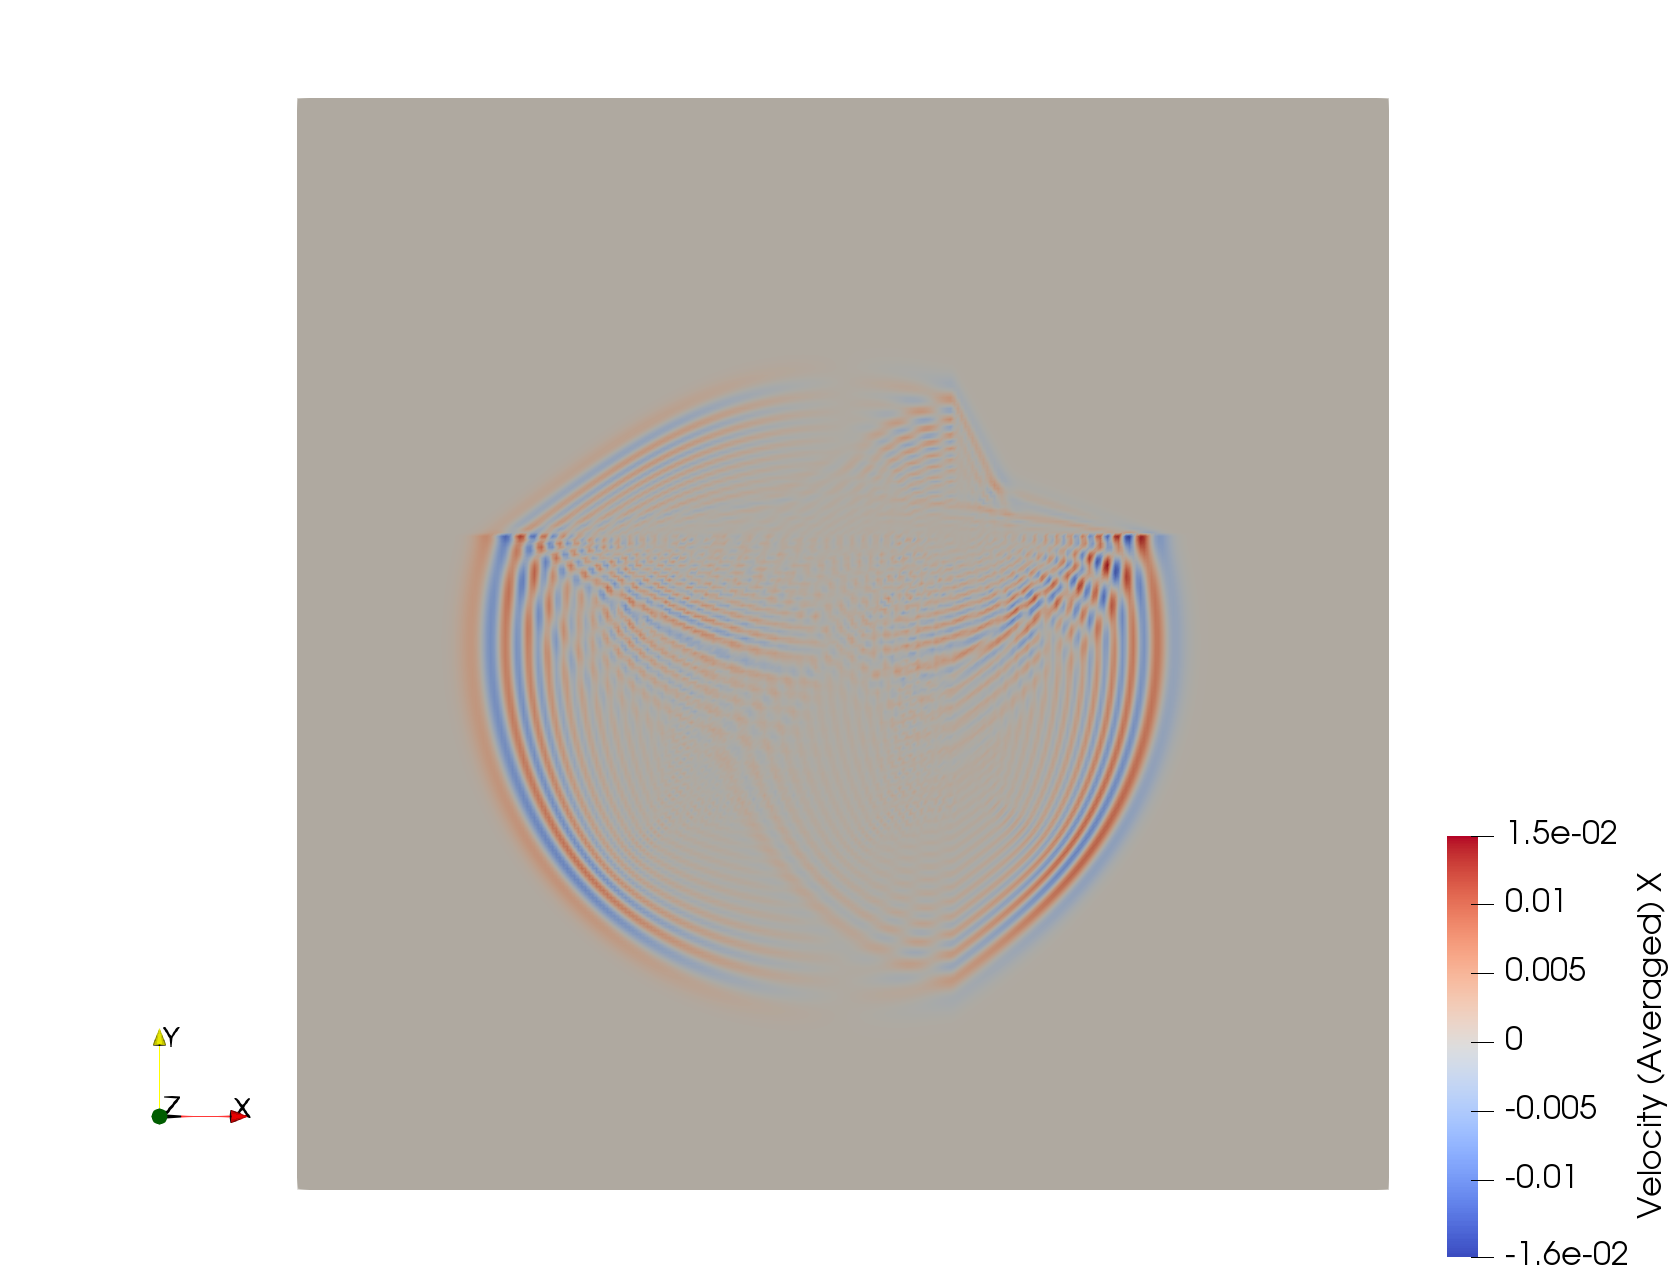
\includegraphics[width=0.4\textwidth]{500_var_x.png}
\end{center}
\begin{lstlisting}[language=bash,basicstyle=\scriptsize\ttfamily]
./ex61 -nsteps 500 -variable -stag_grid_x 300 -stag_grid_y 300 -dt 4e-4
\end{lstlisting}
\end{frame}

%%%%%%%%%%%%%%%%%%%%%%%%%%%%%%%%%%%%%%%%%%%%%%%%%%%%%%%%%%%%%%%%%%%%%%%%%%%%%%%%
%%%%%%%%%%%%%%%%%%%%%%%%%%%%%%%%%%%%%%%%%%%%%%%%%%%%%%%%%%%%%%%%%%%%%%%%%%%%%%%%
\section{Output}

\begin{frame}[fragile]
\frametitle{Output}
  \begin{itemize}
  \item Output is done in a roundabout way, which works but isn't ideal
  \item Functions are provided to convert data associated with a DMStag to data associated with a DMDA
  \item Existing output functionality is used to generate files
  \item PETSc itself isn't heavily concerned with output, so applications (including StagBL) should explore other options
  \item Promising approach in 2D, thanks to Adina P\"{u}s\"{o}k and Dave May: using PETSc's Python-loading scripts, and some custom code to work with data living on DMStag's.
  \end{itemize}
  \begin{center}
  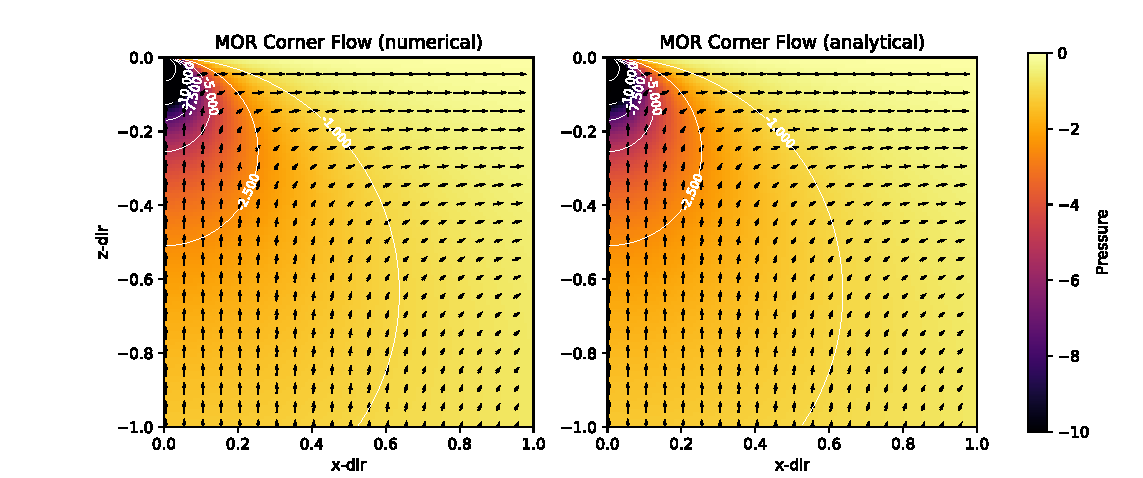
\includegraphics[width=0.6\textwidth]{images/adina_corner_flow.pdf} \\
  {\tiny A. P\"{u}s\"{o}k, University of Oxford}
  \end{center}
\end{frame}

%%%%%%%%%%%%%%%%%%%%%%%%%%%%%%%%%%%%%%%%%%%%%%%%%%%%%%%%%%%%%%%%%%%%%%%%%%%%%%%%
%%%%%%%%%%%%%%%%%%%%%%%%%%%%%%%%%%%%%%%%%%%%%%%%%%%%%%%%%%%%%%%%%%%%%%%%%%%%%%%%
\section{StagBL and StagBLDemo}

%%%%%%%%%%%%%%%%%%%%%%%%%%%%%%%%%%%%%%%%%%%%%%%%%%%%%%%%%%%%%%%%%%%%%%%%%%%%%%%%
\begin{frame}[fragile]
  \frametitlelogo{Building an Application on to of DMStag}
  \begin{itemize}
      \item
  StagBL is a library, built on top of PETSc, including our new DMStag component,
  to make it easier to leverage advanced solvers for staggered-grid geodynamics
  codes.
\item Currently, DMStag does most of the heavy lifting, but the advantage of the StagBL library is that it can provide less-general, and thus easier-to-use, functions (though it currently does not do a great job of this).
  \item
  It includes a demo application, to show how its components may be used.
  We will use this demonstration to introduce topics that we didn't get
  to in the previous lecture, on DMStag:
  \begin{itemize}
      \item Stokes systems
      \item Stokes Solvers
      \item Interaction with Particle systems (DMSwarm)
  \end{itemize}
  \end{itemize}
\end{frame}

\begin{frame}[fragile]
  \frametitlelogo{Demonstration Code}
  \begin{itemize}
      \item
  StagBL contains a demonstration code, which we'll be using.
\item
  While application codes using StagBL do not have to be based on PETSc
  (even though StagBL depends on it), we use PETSc to help us quickly write this demo.
  \end{itemize}
  \begin{center}
  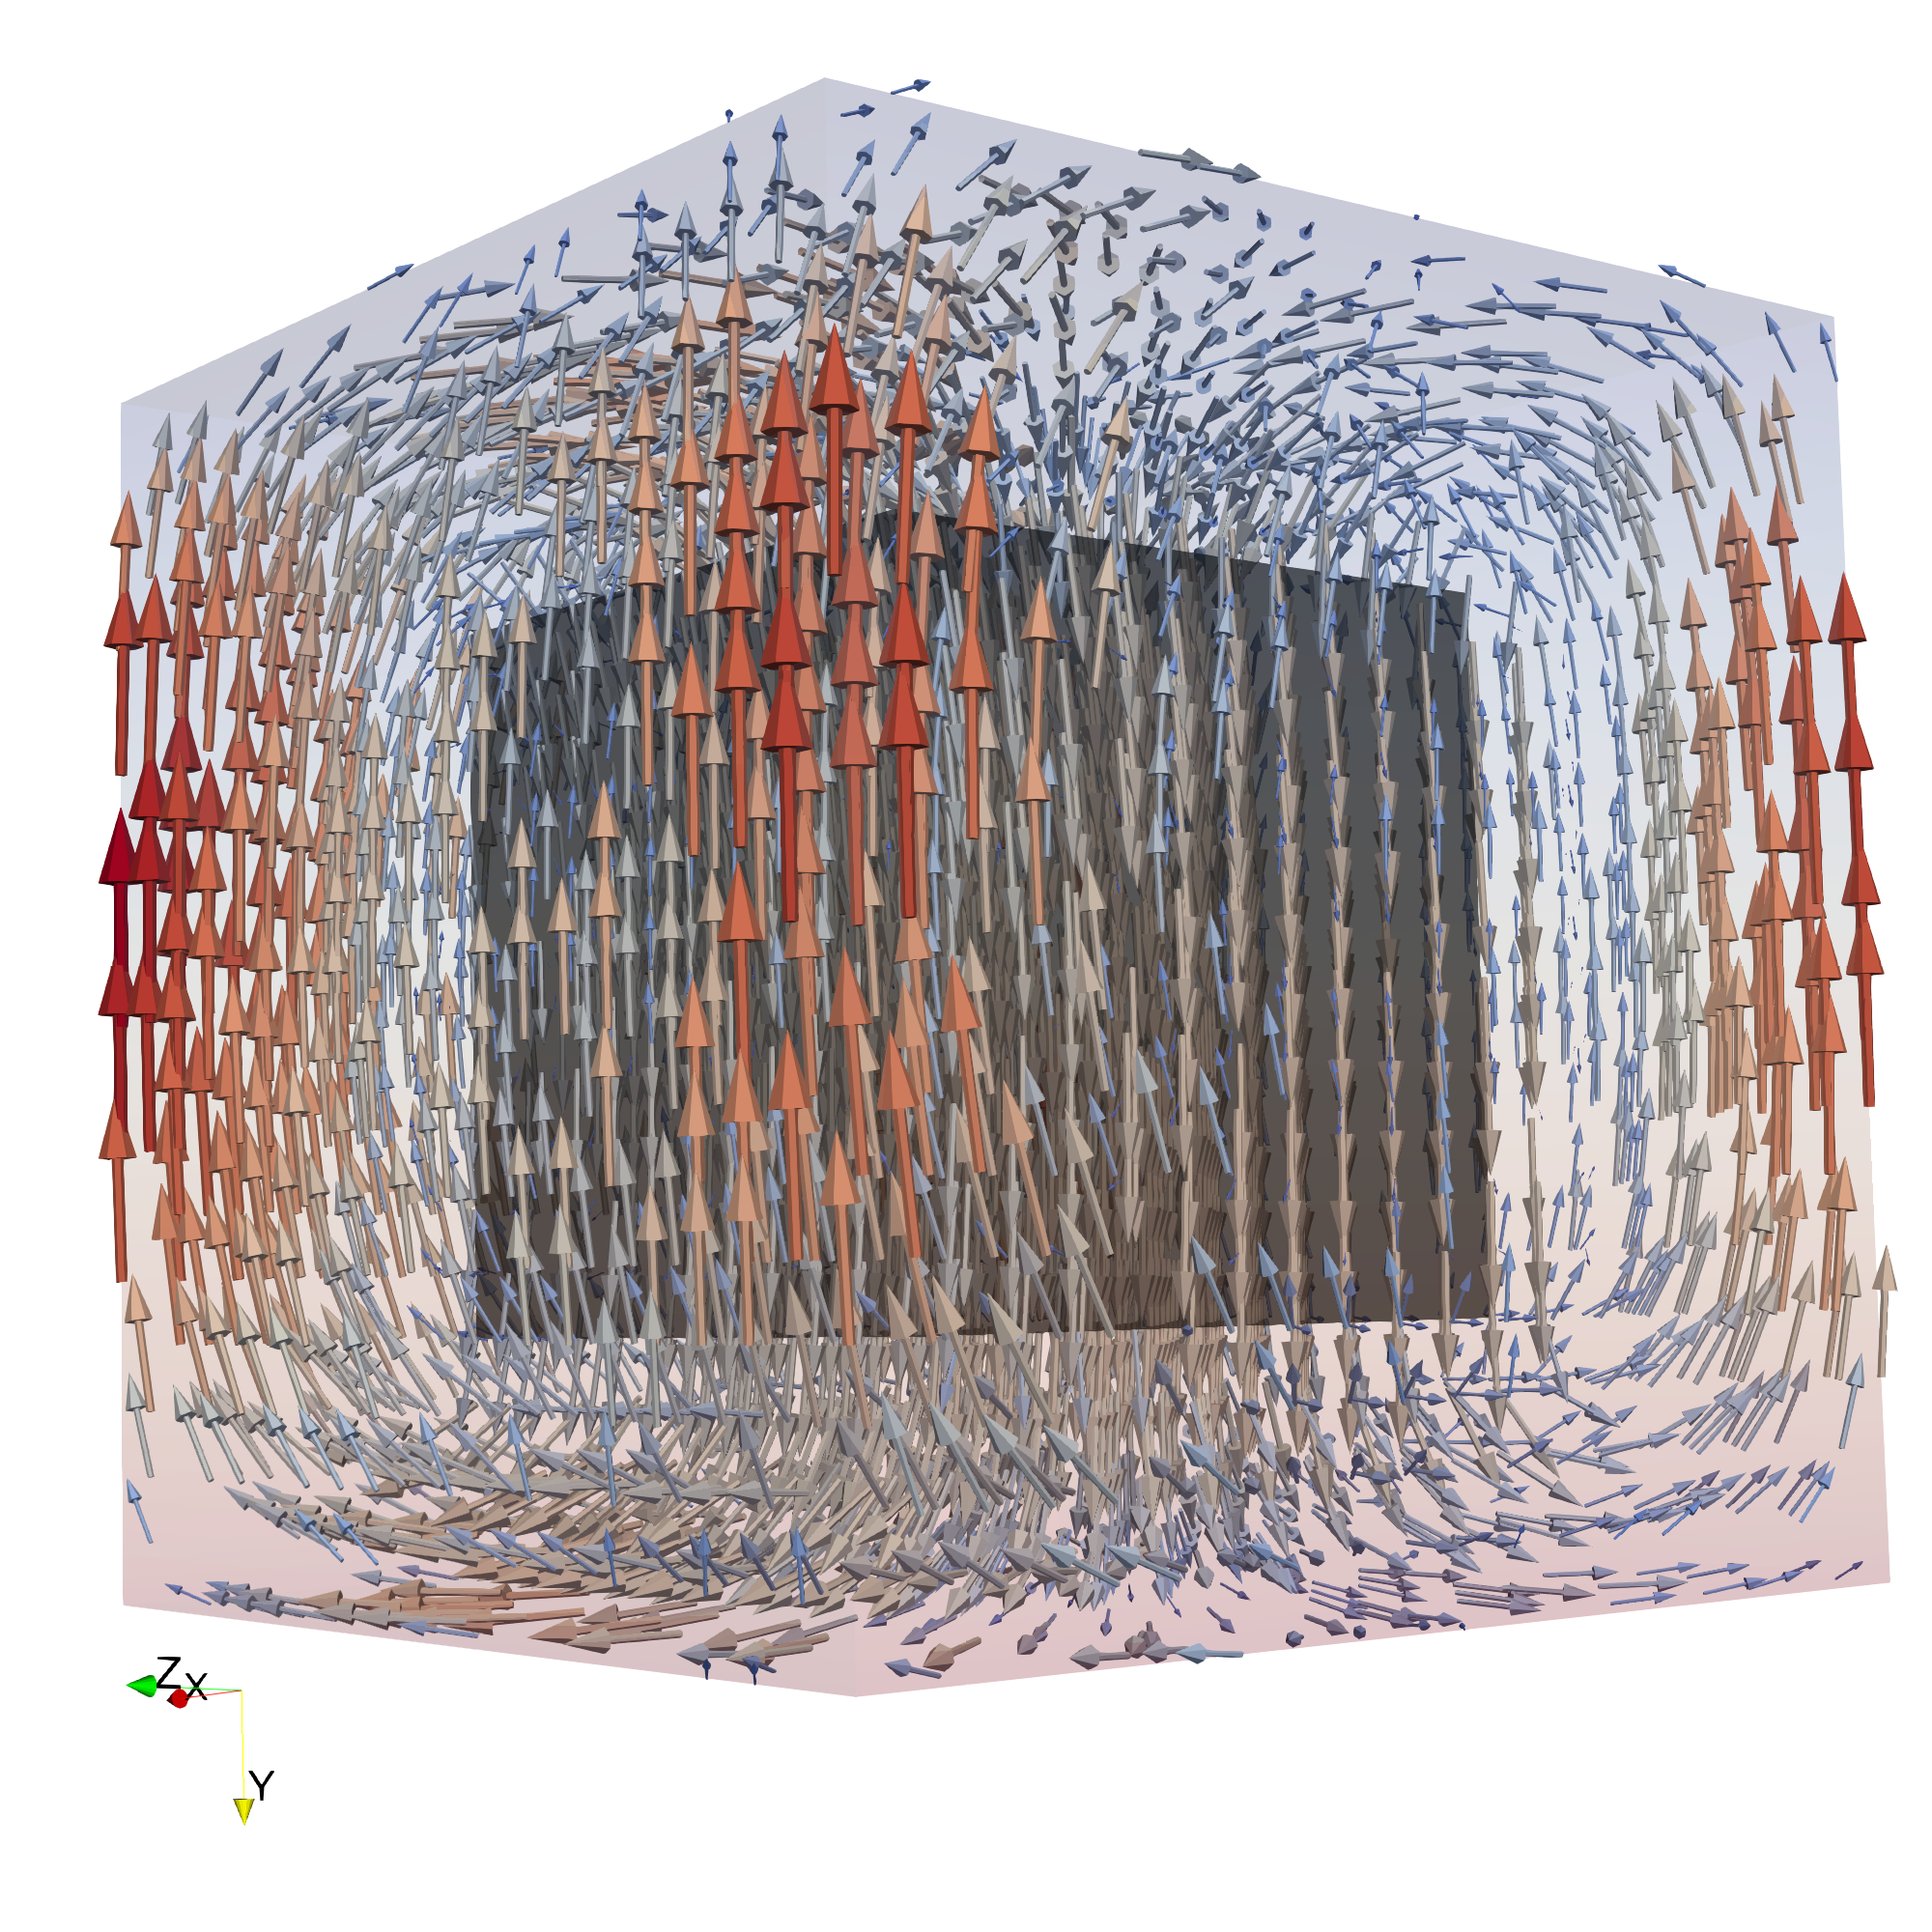
\includegraphics[width=0.4\textwidth]{images/3d_sinker_box_20.png}
  \end{center}

\end{frame}


\begin{frame}[fragile]
  \frametitlelogo{Running the Code}

  \begin{itemize}
  \item Obtain and build a custom version of PETSc, and StagBL, as described at
    \href{github.com/stagbl/stagbl}{https://github.com/stagbl/stagbl}
    \item Run it, as described there, and confirm that you can get the expected output.
  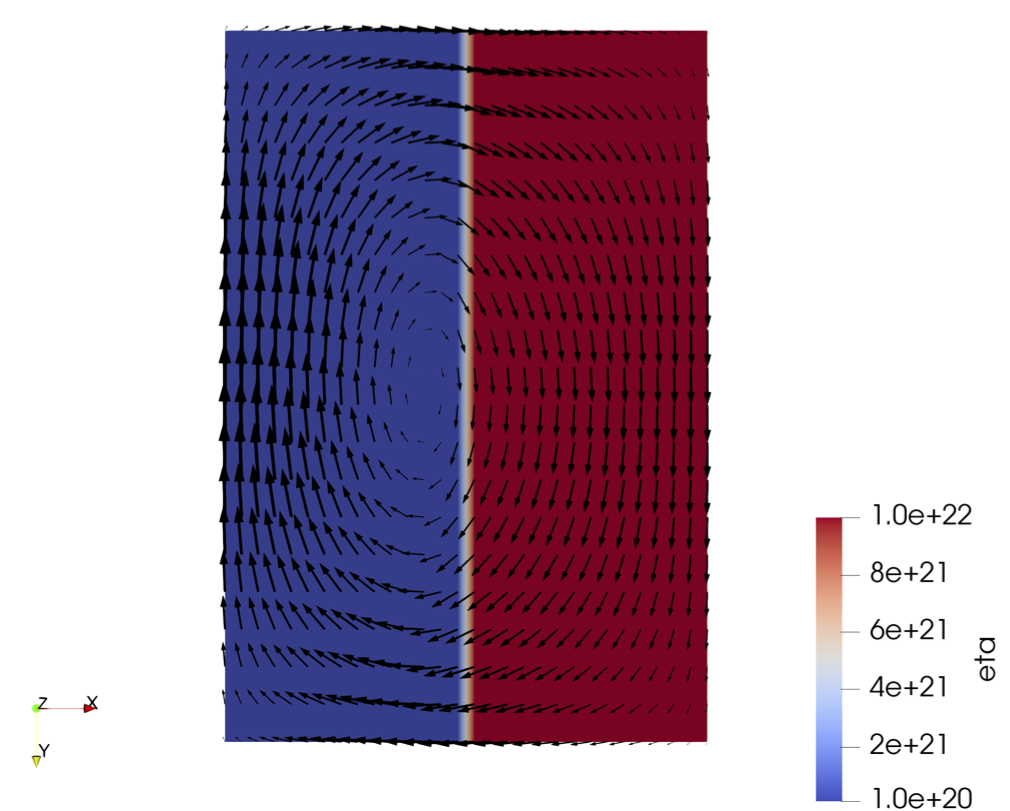
\includegraphics[height=0.4\textheight]{images/stagbldemo2d_quickstart.png}
\item Run it, trying to reproduce the Blankenbach benchmark, using the instructions at
  \href{stagbl.readthedocs.io}{https://stagbl.readthedocs.io/en/latest/benchmarks.html}
  \end{itemize}
\end{frame}

\section{Constructing a Stokes System}

\begin{frame}[fragile]
  \frametitlelogo{Using DMStag to Create an Operator}
StagBL currently uses DMStag directly to construct Stokes operators in a simple case.
\begin{lstlisting}[language=bash,basicstyle=\tiny\ttfamily]
% From src/stokes/stokes.c
PetscErrorCode StagBLCreateStokesSystem(StagBLStokesParameters parameters, StagBLSystem *system)
{
  PetscErrorCode ierr;
  DM             dm_stokes;
  PetscInt       dim;

  PetscFunctionBegin;
  ierr = StagBLGridPETScGetDM(parameters->stokes_grid,&dm_stokes);CHKERRQ(ierr);
  ierr = DMGetDimension(dm_stokes,&dim);CHKERRQ(ierr);
  ierr = StagBLGridCreateStagBLSystem(parameters->stokes_grid,system);CHKERRQ(ierr);
  switch (dim) {
    case 2:
    ierr = CreateSystem_2D_FreeSlip(parameters,*system);CHKERRQ(ierr);
  break;
    case 3:
    ierr = CreateSystem_3D_FreeSlip(parameters,*system);CHKERRQ(ierr);
    break;
    default: StagBLError1(PetscObjectComm((PetscObject)dm_stokes),"Unsupported dimension %D",dim);
  }
  PetscFunctionReturn(0);
}
\end{lstlisting}
Let's take a look at this function and how it's used in the demo.
\end{frame}

\section{Solving the Stokes System}

\begin{frame}[fragile]
\frametitlelogo{Solving the Stokes System}
\begin{itemize}
\item Once the system is assembled, we have the power of PETSc
\item We wrap the solver object in our core \lstinline{StagBLSolver} class (see
\href{stagbl.readthedocs.io}{https://stagbl.readthedocs.io/en/latest/benchmarks.html})
\item Let's look at all the solvers from the command line\footnote{currently not using options prefixes correctly!}
  \begin{lstlisting}
./stagbldemo2d -ksp_view
  \end{lstlisting}
\item In the simplest case (the current demo), we can use a direct solver
\item Let's see how this is done
\item However, the real point of StagBL is to enable advanced solvers, as we saw early with our DMDA multigrid example, so let's look at some work-in-progress..
\end{itemize}
\end{frame}
\begin{frame}[fragile]
\frametitlelogo{Solving the Stokes System}
\begin{itemize}
\item Once the system is assembled, we have the power of PETSc
\item In the simplest case (the current demo), we can use a direct solver
\item Let's see how this is done
\item However, the real point of StagBL is to enable advanced solvers, as we saw early with our DMDA multigrid example..
\end{itemize}
\end{frame}
\begin{frame}[fragile]
  \frametitlelogo{Multigrid Components}

  Optimal transfer operators will vary with the particular problem,
  but we provide widely-used choices (e.g. \footfullcite[App. C]{CaiEtAl2014})
  appropriate for MAC Stokes flow.

  \begin{enumerate}
    \item  Injection/averaging for element-based values (~pressures)
    \item  Interpolation on faces (~velocities) is linear for faces overlaying coarse faces, and bilinear otherwise
    \item Restriction for faces is also bilinear
  \end{enumerate}
  \begin{center}
  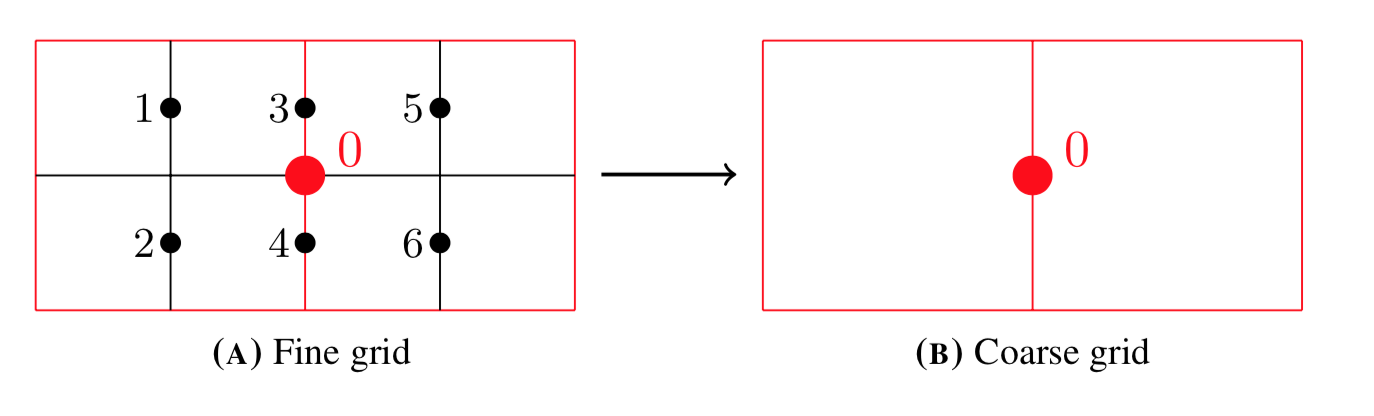
\includegraphics[width=0.7\textwidth]{images/Chen2018restrict.png} \footfullcite{Chen2018}
  \end{center}

\end{frame}

\begin{frame}[fragile]
\frametitlelogo{ABF + Multigrid Test Case}
\begin{center}
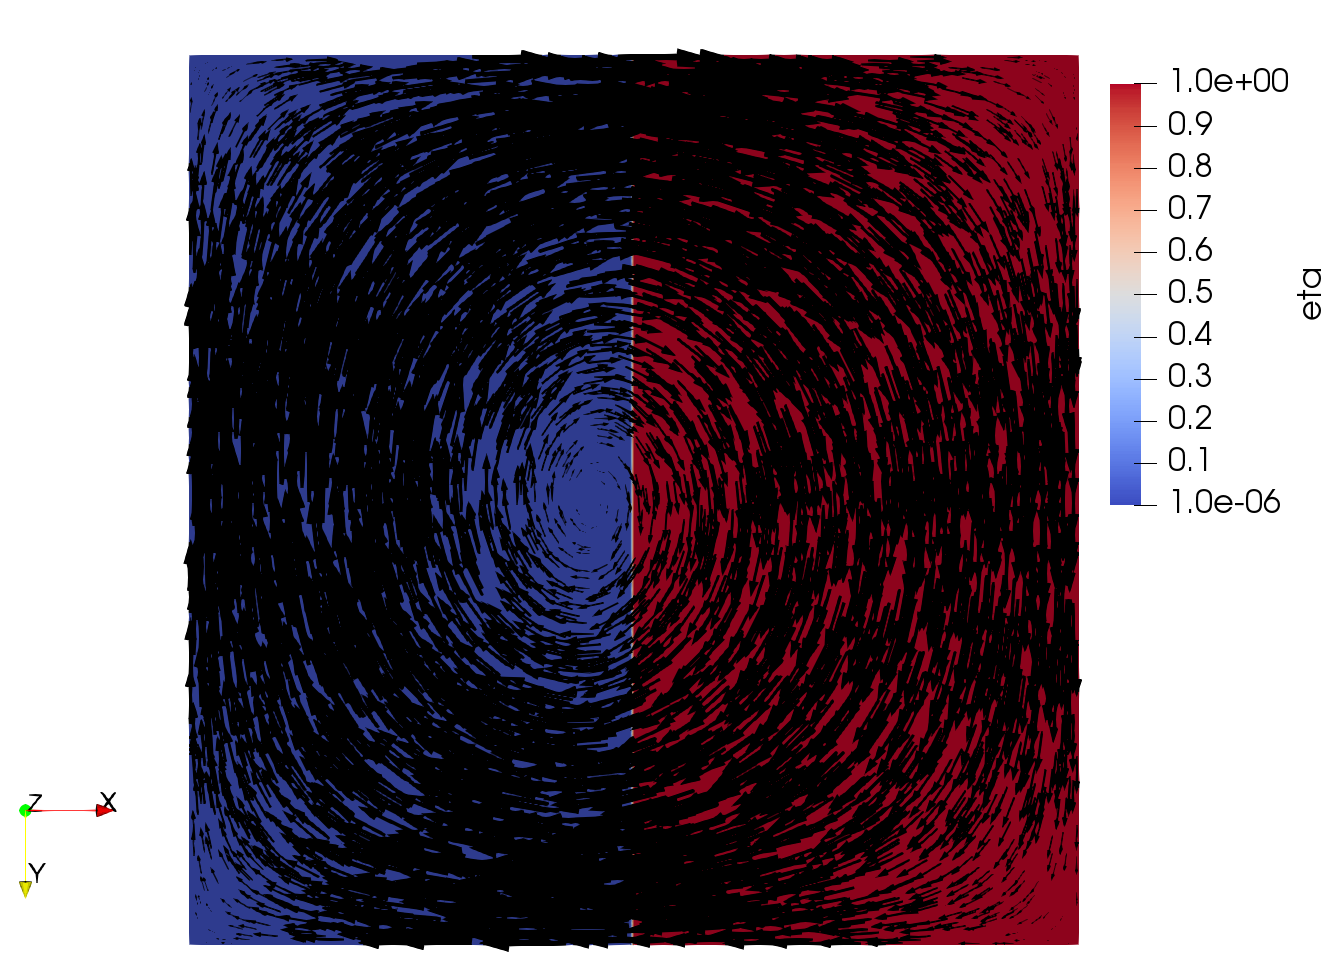
\includegraphics[width=0.45\textwidth]{images/ex4_1e6.png}\\
$ \eta_1 \leftarrow \rightarrow \eta_2$
\end{center}
\begin{itemize}
\item DMStag tutorial \texttt{ex4}, based on textbook exercise \footfullcite[ex. 7.2]{Gerya2009}
\item Variable-viscosity bouyancy-driven Stokes flow, free-slip boundary conditions
\item modified to
\begin{itemize}
\item Incorporate proper pressure nullspace
\item Use non-dimensional units
\item Construct diagonal auxiliary matrix, with entries as inverse viscosity
\end{itemize}
\end{itemize}
\end{frame}

\begin{frame}[fragile]
\frametitlelogo{ABF + Multigrid Test Case: Isoviscous}
\begin{lstlisting}[language=bash,basicstyle=\scriptsize\ttfamily]
-nondimensional
-isoviscous
-stag_grid_x 256
-stag_grid_y 256
-ksp_type fgmres
-pc_type fieldsplit
-pc_fieldsplit_type schur
-pc_fieldsplit_schur_fact_type upper
-pc_fieldsplit_schur_precondition user #  Diagonal inverse-viscosity approximation
-fieldsplit_element_ksp_type preonly
-fieldsplit_element_pc_type jacobi
-fieldsplit_face_pc_type mg
-fieldsplit_face_pc_mg_levels 5
-fieldsplit_face_pc_mg_galerkin
-fieldsplit_face_mg_levels_pc_type jacobi
-fieldsplit_face_mg_levels_ksp_type chebyshev
\end{lstlisting}
\end{frame}

% See experiments in DMStag paper repo
\begin{frame}[fragile]
\frametitlelogo{ABF + Multigrid Test Case: Isoviscous}
  Set $\eta_1 = \eta_2 = 1$ and run on Piz Daint
\begin{table}[]
\begin{tabular}{lllll}
  Grid &  Ranks & MG Levels & FGMRES Its. ($10^{-6}$ rel. tol.) &  \texttt{KSPSolve} time  [s]  \\
\hline
  $256^2$  & $4$    & $5$  & $5$ & 0.23  \\
  $512^2$  & $16$   & $6$  & $5$ & 0.32  \\
  $1024^2$ & $64$   & $7$  & $5$ & 0.42  \\
  $2048^2$ & $256$  & $8$  & $5$ & 1.06  \\
  $4096^2$ & $1024$ & $8$* & $7$ & 1.98\\
\end{tabular}
\end{table}

  * At this point, one should use \texttt{PCTelescope} \footfullcite{MayEtAl2016}.

\end{frame}

\begin{frame}[fragile]
\frametitlelogo{ABF + Multigrid Test Case: Variable Viscosity}
\begin{lstlisting}[language=bash,basicstyle=\scriptsize\ttfamily]
-nondimensional
-eta1 1e-6 # Set viscosity contrast
-stag_grid_x 256
-stag_grid_y 256
-ksp_type fgmres
-pc_type fieldsplit
-pc_fieldsplit_type schur
-pc_fieldsplit_schur_fact_type upper
-pc_fieldsplit_schur_precondition selfp
-fieldsplit_element_ksp_type preonly
-fieldsplit_element_pc_type jacobi
-fieldsplit_face_pc_type mg
-fieldsplit_face_pc_mg_galerkin
-fieldsplit_face_pc_mg_levels 5
-fieldsplit_face_mg_levels_ksp_max_it 6
-fieldsplit_face_mg_levels_ksp_type chebyshev
-fieldsplit_face_mg_levels_pc_type jacobi
-fieldsplit_face_mg_coarse_pc_type redundant
-fieldsplit_face_mg_coarse_redundant_pc_type lu
-fieldsplit_face_mg_coarse_redundant_pc_factor_mat_solver_type umfpack
\end{lstlisting}
\end{frame}

% Run on pdsbox

%commit 28e3855a99d4380a0cab4441278d344239aab33d (HEAD -> psanan/dmstag-mg-2)
%Author: Patrick Sanan <patrick.sanan@gmail.com>
%Date:   Thu Oct 17 23:21:27 2019 +0100
%
%    DMStag ex4: add options to set viscosities

% Debug
% $PMPI -n 1 ./ex4  -pc_type fieldsplit -pc_fieldsplit_type schur -ksp_converged_reason -fieldsplit_element_ksp_type preonly  -pc_fieldsplit_detect_saddle_point false -fieldsplit_face_pc_type mg -fieldsplit_face_pc_mg_levels 5 -fieldsplit_face_pc_mg_galerkin -fieldsplit_face_mg_coarse_pc_type redundant -fieldsplit_face_mg_coarse_redundant_pc_type lu -fieldsplit_face_mg_coarse_redundant_pc_factor_mat_solver_type umfpack  -ksp_type fgmres -fieldsplit_element_pc_type none -fieldsplit_face_mg_levels_ksp_max_it 6 -pc_fieldsplit_schur_fact_type upper -nondimensional -ksp_monitor -options_left -fieldsplit_face_mg_levels_pc_type jacobi -fieldsplit_face_mg_levels_ksp_type chebyshev -fieldsplit_element_pc_type jacobi -pc_fieldsplit_schur_precondition selfp   -stag_grid_x 128 -stag_grid_y 128 -fieldsplit_face_ksp_monitor  -eta1 1e-6

%Run
% $PMPI -n 1 ./ex4  -pc_type fieldsplit -pc_fieldsplit_type schur -fieldsplit_element_ksp_type preonly  -pc_fieldsplit_detect_saddle_point false -fieldsplit_face_pc_type mg -fieldsplit_face_pc_mg_levels 5 -fieldsplit_face_pc_mg_galerkin -fieldsplit_face_mg_coarse_pc_type redundant -fieldsplit_face_mg_coarse_redundant_pc_type lu -fieldsplit_face_mg_coarse_redundant_pc_factor_mat_solver_type umfpack  -ksp_type fgmres -fieldsplit_element_pc_type none -fieldsplit_face_mg_levels_ksp_max_it 6 -pc_fieldsplit_schur_fact_type upper -nondimensional -fieldsplit_face_mg_levels_pc_type jacobi -fieldsplit_face_mg_levels_ksp_type chebyshev -fieldsplit_element_pc_type jacobi -pc_fieldsplit_schur_precondition selfp   -stag_grid_x 128 -stag_grid_y 128 -eta1 1e-6 -log_view ascii:log.txt

\begin{frame}[fragile]
\frametitlelogo{ABF + Multigrid Test Case: Viscosity Jump}
  With a viscosity jump of 6 orders of magnitude, $\eta_1 = 10^{-6}, \eta_2 = 1$,
  we see good algorithmic scalability:
    \begin{table}[]
\begin{tabular}{lllll}
  Grid &  MG Levels & FGMRES Iterations ($10^-6$ rel. tol.) &  \texttt{KSPSolve} time [s]  \\
  \hline
   $32^2$  & 3 &  12 & 0.025 \\
   $64^2$  & 4 &  12 & 0.11 \\
   $128^2$  & 5 &  12 & 0.48 \\
   $256^2$  & 6 &  11 & 2.05 \\
   $512^2$  & 7 &  11 & 9.56 \\
   $1024^2$ & 8 &  11 & 41.2 \\
\end{tabular}
\end{table}
Run on a single rank on a desktop, but identical iteration counts in parallel.

\end{frame}

\begin{frame}[fragile]
  \frametitlelogo{Current Work: Monolithic Smoothers}
  \begin{itemize}
  \item \texttt{DMStag}'s default interpolation operators are suitable for geometric multigrid on the entire saddle point matrix
  \item An important smoother in this case is the Distributed Gauss-Seidel (DGS) smoother \footfullcite{BrandtDinar1979} and related algorithms \footfullcite{WangChen2013}.
    \item These are not quite available from the command line, though they are extremely similar to ABF preconditioners
  \item Thus, we will introduce a new implementation of \texttt{PCFieldSplit} to support preconditioners of the following form , for an operator $L$:
    $$
      P = M\hat{(LM)}^{-1}
      $$

      \begin{equation*} \label{eq:LM}
  LM =  \mattwo{A}{G}{D}{} \underbrace{\mattwo{I}{G}{}{-DG}}_M = \mattwo{A}{AG-GDG}{D}{DG}
\end{equation*}

  \end{itemize}
\end{frame}

%\begin{frame}[fragile]
%  \frametitlelogo{Current Work: 2-phase flow}
%  \begin{itemize}
%    \item \texttt{DMStag} can provide a platform to construct a 2-phase flow model
%    \item In a simple formulation (currently being written as a PETSc example),
%      one may solve equations in the form of an augmented Stokes system
%$$
%\begin{bmatrix}
%A 	&  G \\
%D 	&  C
%\end{bmatrix}
%\begin{bmatrix}
%u \\
%p
%\end{bmatrix}
%=
%\begin{bmatrix}
%f \\
%g
%\end{bmatrix},
%\quad \text{or } \mathcal{A} v = {\mathcal F}
%$$
%  \end{itemize}
%  \begin{center}
%    \includegraphics[width=0.5\textwidth]{images/SM1987.png}\footfullcite{SpiegelmanMcKenzie1987}
%  \end{center}
%\end{frame}


\section{Interacting with Particles}

\section{Particles with \texttt{DMSwarm}}

\begin{frame}[fragile]
\frametitlelogo{Particle Integration}
  \begin{itemize}
    \item By integrating with \PETSc{}'s \texttt{DMSwarm}, one can buld a full MAC code with \texttt{DMStag}
    \item Particles store a cell ID, coordinates, and other data
    \item Coordinates represented using \texttt{DMProduct} allow fast location of particles
    \item \lstinline{DMStagMigrate()} takes care of parallel details
      \item Default interpolation routines are provided
    \item For an example, see
\lstinline{$PETSC_DIR/src/dm/impls/stag/examples/tutorials/ex5.c}
(in the \texttt{psanan/stagbl-working-base} branch, currently)
  \end{itemize}
\end{frame}


\begin{frame}[fragile]
  \frametitlelogo{Particles with StagBLDemo2d}
  \begin{itemize}
      \item Our 2D demo includes particles, but not in a `full-featured` way
        \item Temperature is interpolated to the particles from the grid
        \item Information isn't propagated the other way, yet, though the tools are in place (hackathon topic for me?)
        \item Let's look at \texttt{src/demos/particles.c}
  \end{itemize}
  \begin{center}
    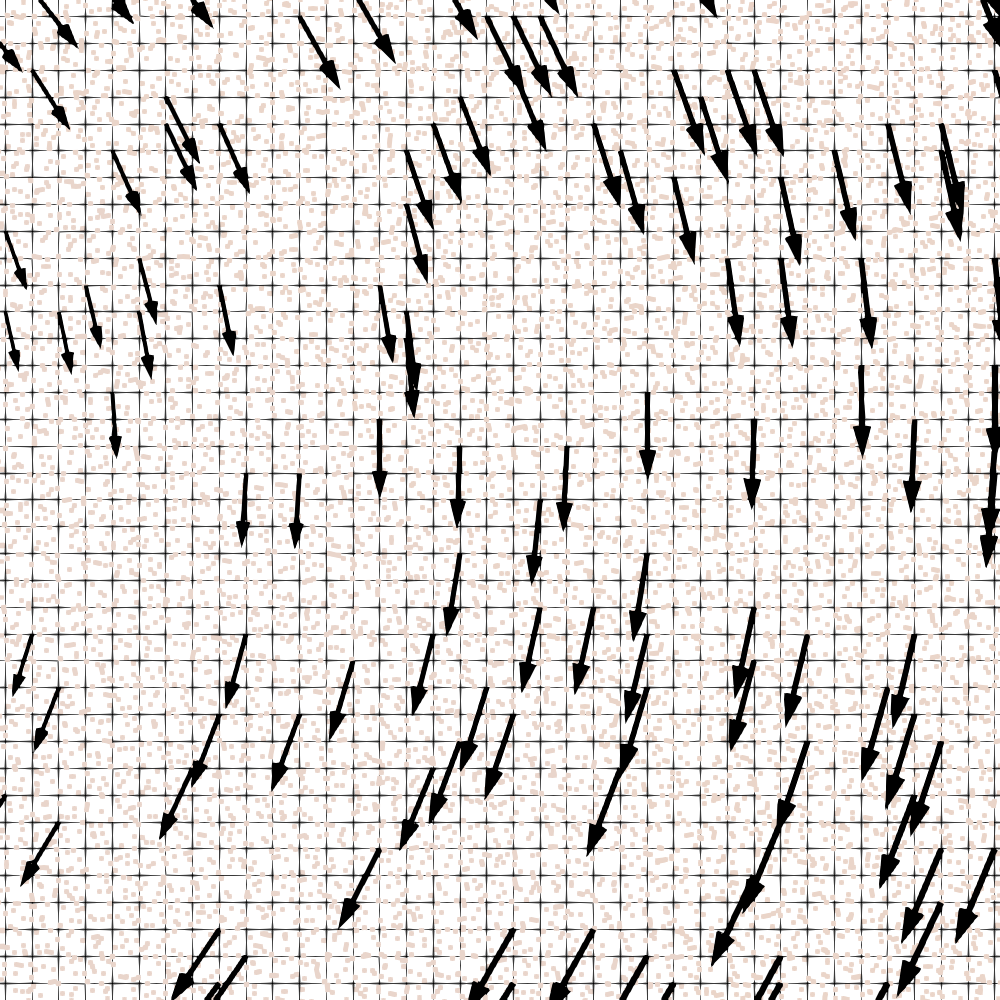
\includegraphics[width=0.3\textwidth]{images/2d_particles_closeup.png}
  \end{center}
\end{frame}

\end{document}
